\documentclass[preprint, 10pt]{article}


\usepackage[dvipsnames]{xcolor}
\usepackage[accepted]{tmlr}
\usepackage{amsmath}
\usepackage[utf8]{inputenc} % allow utf-8 input
\usepackage[T1]{fontenc}    % use 8-bit T1 fonts
\usepackage[colorlinks=true,urlcolor=blue,citecolor=blue]{hyperref}       % hyperlinks
\usepackage{url}            % simple URL typesetting
\usepackage{booktabs}       % professional-quality tables
\usepackage{amsfonts}       % blackboard math symbols
\usepackage{nicefrac}       % compact symbols for 1/2, etc.
\usepackage{microtype}      % microtypography
\usepackage{cleveref}       % smart cross-referencing
\usepackage{lipsum}         % Can be removed after putting your text content
\usepackage{graphicx}
\usepackage{acronym}
\usepackage{tikz}
\usepackage{bbm}
\usepackage[skip=2pt]{caption}
\usepackage{subcaption}
\usepackage{algorithm} 
\usepackage{algpseudocode}
\usepackage[toc,page]{appendix}
\usepackage{wrapfig}
\setcitestyle{sort, yearnat}
\usepackage[inline]{enumitem}
\usepackage[normalem]{ulem}
\usepackage{titlesec}
\usepackage{titlecaps}
\usepackage{fancyhdr}
\usepackage{pifont}
% for printing numbers
\usepackage{numprint}
\npthousandsep{,}
\npdecimalsign{.}
\usepackage{comment} % multi-line comments
\usepackage{longtable}

% math
\usepackage{amsthm}
\usepackage{mathtools}
\usepackage{amssymb}

\newtheorem{proposition}{Proposition}
\newtheorem{assumption}{Assumption}
\newtheorem{theorem}{Theorem}[section]
\newtheorem{innercustomthm}{Theorem}
\newenvironment{thm}[1]
{\renewcommand\theinnercustomthm{#1}\innercustomthm}
{\endinnercustomthm}

\usepackage{natbib}
\PassOptionsToPackage{sort&compress}{natbib} 

%%%%% NEW MATH DEFINITIONS %%%%%

\usepackage{amsmath,amsfonts,bm}

% Mark sections of captions for referring to divisions of figures
\newcommand{\figleft}{{\em (Left)}}
\newcommand{\figcenter}{{\em (Center)}}
\newcommand{\figright}{{\em (Right)}}
\newcommand{\figtop}{{\em (Top)}}
\newcommand{\figbottom}{{\em (Bottom)}}
\newcommand{\captiona}{{\em (a)}}
\newcommand{\captionb}{{\em (b)}}
\newcommand{\captionc}{{\em (c)}}
\newcommand{\captiond}{{\em (d)}}

% Highlight a newly defined term
\newcommand{\newterm}[1]{{\bf #1}}


% Figure reference, lower-case.
\def\figref#1{figure~\ref{#1}}
% Figure reference, capital. For start of sentence
\def\Figref#1{Figure~\ref{#1}}
\def\twofigref#1#2{figures \ref{#1} and \ref{#2}}
\def\quadfigref#1#2#3#4{figures \ref{#1}, \ref{#2}, \ref{#3} and \ref{#4}}
% Section reference, lower-case.
\def\secref#1{section~\ref{#1}}
% Section reference, capital.
\def\Secref#1{Section~\ref{#1}}
% Reference to two sections.
\def\twosecrefs#1#2{sections \ref{#1} and \ref{#2}}
% Reference to three sections.
\def\secrefs#1#2#3{sections \ref{#1}, \ref{#2} and \ref{#3}}
% Reference to an equation, lower-case.
\def\eqref#1{equation~\ref{#1}}
% Reference to an equation, upper case
\def\Eqref#1{Equation~\ref{#1}}
% A raw reference to an equation---avoid using if possible
\def\plaineqref#1{\ref{#1}}
% Reference to a chapter, lower-case.
\def\chapref#1{chapter~\ref{#1}}
% Reference to an equation, upper case.
\def\Chapref#1{Chapter~\ref{#1}}
% Reference to a range of chapters
\def\rangechapref#1#2{chapters\ref{#1}--\ref{#2}}
% Reference to an algorithm, lower-case.
\def\algref#1{algorithm~\ref{#1}}
% Reference to an algorithm, upper case.
\def\Algref#1{Algorithm~\ref{#1}}
\def\twoalgref#1#2{algorithms \ref{#1} and \ref{#2}}
\def\Twoalgref#1#2{Algorithms \ref{#1} and \ref{#2}}
% Reference to a part, lower case
\def\partref#1{part~\ref{#1}}
% Reference to a part, upper case
\def\Partref#1{Part~\ref{#1}}
\def\twopartref#1#2{parts \ref{#1} and \ref{#2}}

\def\ceil#1{\lceil #1 \rceil}
\def\floor#1{\lfloor #1 \rfloor}
\def\1{\bm{1}}
\newcommand{\train}{\mathcal{D}}
\newcommand{\valid}{\mathcal{D_{\mathrm{valid}}}}
\newcommand{\test}{\mathcal{D_{\mathrm{test}}}}

\def\eps{{\epsilon}}


% Random variables
\def\reta{{\textnormal{$\eta$}}}
\def\ra{{\textnormal{a}}}
\def\rb{{\textnormal{b}}}
\def\rc{{\textnormal{c}}}
\def\rd{{\textnormal{d}}}
\def\re{{\textnormal{e}}}
\def\rf{{\textnormal{f}}}
\def\rg{{\textnormal{g}}}
\def\rh{{\textnormal{h}}}
\def\ri{{\textnormal{i}}}
\def\rj{{\textnormal{j}}}
\def\rk{{\textnormal{k}}}
\def\rl{{\textnormal{l}}}
% rm is already a command, just don't name any random variables m
\def\rn{{\textnormal{n}}}
\def\ro{{\textnormal{o}}}
\def\rp{{\textnormal{p}}}
\def\rq{{\textnormal{q}}}
\def\rr{{\textnormal{r}}}
\def\rs{{\textnormal{s}}}
\def\rt{{\textnormal{t}}}
\def\ru{{\textnormal{u}}}
\def\rv{{\textnormal{v}}}
\def\rw{{\textnormal{w}}}
\def\rx{{\textnormal{x}}}
\def\ry{{\textnormal{y}}}
\def\rz{{\textnormal{z}}}

% Random vectors
\def\rvepsilon{{\mathbf{\epsilon}}}
\def\rvtheta{{\mathbf{\theta}}}
\def\rva{{\mathbf{a}}}
\def\rvb{{\mathbf{b}}}
\def\rvc{{\mathbf{c}}}
\def\rvd{{\mathbf{d}}}
\def\rve{{\mathbf{e}}}
\def\rvf{{\mathbf{f}}}
\def\rvg{{\mathbf{g}}}
\def\rvh{{\mathbf{h}}}
\def\rvu{{\mathbf{i}}}
\def\rvj{{\mathbf{j}}}
\def\rvk{{\mathbf{k}}}
\def\rvl{{\mathbf{l}}}
\def\rvm{{\mathbf{m}}}
\def\rvn{{\mathbf{n}}}
\def\rvo{{\mathbf{o}}}
\def\rvp{{\mathbf{p}}}
\def\rvq{{\mathbf{q}}}
\def\rvr{{\mathbf{r}}}
\def\rvs{{\mathbf{s}}}
\def\rvt{{\mathbf{t}}}
\def\rvu{{\mathbf{u}}}
\def\rvv{{\mathbf{v}}}
\def\rvw{{\mathbf{w}}}
\def\rvx{{\mathbf{x}}}
\def\rvy{{\mathbf{y}}}
\def\rvz{{\mathbf{z}}}

% Elements of random vectors
\def\erva{{\textnormal{a}}}
\def\ervb{{\textnormal{b}}}
\def\ervc{{\textnormal{c}}}
\def\ervd{{\textnormal{d}}}
\def\erve{{\textnormal{e}}}
\def\ervf{{\textnormal{f}}}
\def\ervg{{\textnormal{g}}}
\def\ervh{{\textnormal{h}}}
\def\ervi{{\textnormal{i}}}
\def\ervj{{\textnormal{j}}}
\def\ervk{{\textnormal{k}}}
\def\ervl{{\textnormal{l}}}
\def\ervm{{\textnormal{m}}}
\def\ervn{{\textnormal{n}}}
\def\ervo{{\textnormal{o}}}
\def\ervp{{\textnormal{p}}}
\def\ervq{{\textnormal{q}}}
\def\ervr{{\textnormal{r}}}
\def\ervs{{\textnormal{s}}}
\def\ervt{{\textnormal{t}}}
\def\ervu{{\textnormal{u}}}
\def\ervv{{\textnormal{v}}}
\def\ervw{{\textnormal{w}}}
\def\ervx{{\textnormal{x}}}
\def\ervy{{\textnormal{y}}}
\def\ervz{{\textnormal{z}}}

% Random matrices
\def\rmA{{\mathbf{A}}}
\def\rmB{{\mathbf{B}}}
\def\rmC{{\mathbf{C}}}
\def\rmD{{\mathbf{D}}}
\def\rmE{{\mathbf{E}}}
\def\rmF{{\mathbf{F}}}
\def\rmG{{\mathbf{G}}}
\def\rmH{{\mathbf{H}}}
\def\rmI{{\mathbf{I}}}
\def\rmJ{{\mathbf{J}}}
\def\rmK{{\mathbf{K}}}
\def\rmL{{\mathbf{L}}}
\def\rmM{{\mathbf{M}}}
\def\rmN{{\mathbf{N}}}
\def\rmO{{\mathbf{O}}}
\def\rmP{{\mathbf{P}}}
\def\rmQ{{\mathbf{Q}}}
\def\rmR{{\mathbf{R}}}
\def\rmS{{\mathbf{S}}}
\def\rmT{{\mathbf{T}}}
\def\rmU{{\mathbf{U}}}
\def\rmV{{\mathbf{V}}}
\def\rmW{{\mathbf{W}}}
\def\rmX{{\mathbf{X}}}
\def\rmY{{\mathbf{Y}}}
\def\rmZ{{\mathbf{Z}}}

% Elements of random matrices
\def\ermA{{\textnormal{A}}}
\def\ermB{{\textnormal{B}}}
\def\ermC{{\textnormal{C}}}
\def\ermD{{\textnormal{D}}}
\def\ermE{{\textnormal{E}}}
\def\ermF{{\textnormal{F}}}
\def\ermG{{\textnormal{G}}}
\def\ermH{{\textnormal{H}}}
\def\ermI{{\textnormal{I}}}
\def\ermJ{{\textnormal{J}}}
\def\ermK{{\textnormal{K}}}
\def\ermL{{\textnormal{L}}}
\def\ermM{{\textnormal{M}}}
\def\ermN{{\textnormal{N}}}
\def\ermO{{\textnormal{O}}}
\def\ermP{{\textnormal{P}}}
\def\ermQ{{\textnormal{Q}}}
\def\ermR{{\textnormal{R}}}
\def\ermS{{\textnormal{S}}}
\def\ermT{{\textnormal{T}}}
\def\ermU{{\textnormal{U}}}
\def\ermV{{\textnormal{V}}}
\def\ermW{{\textnormal{W}}}
\def\ermX{{\textnormal{X}}}
\def\ermY{{\textnormal{Y}}}
\def\ermZ{{\textnormal{Z}}}

% Vectors
\def\vzero{{\bm{0}}}
\def\vone{{\bm{1}}}
\def\vmu{{\bm{\mu}}}
\def\vtheta{{\bm{\theta}}}
\def\va{{\bm{a}}}
\def\vb{{\bm{b}}}
\def\vc{{\bm{c}}}
\def\vd{{\bm{d}}}
\def\ve{{\bm{e}}}
\def\vf{{\bm{f}}}
\def\vg{{\bm{g}}}
\def\vh{{\bm{h}}}
\def\vi{{\bm{i}}}
\def\vj{{\bm{j}}}
\def\vk{{\bm{k}}}
\def\vl{{\bm{l}}}
\def\vm{{\bm{m}}}
\def\vn{{\bm{n}}}
\def\vo{{\bm{o}}}
\def\vp{{\bm{p}}}
\def\vq{{\bm{q}}}
\def\vr{{\bm{r}}}
\def\vs{{\bm{s}}}
\def\vt{{\bm{t}}}
\def\vu{{\bm{u}}}
\def\vv{{\bm{v}}}
\def\vw{{\bm{w}}}
\def\vx{{\bm{x}}}
\def\vy{{\bm{y}}}
\def\vz{{\bm{z}}}

% Elements of vectors
\def\evalpha{{\alpha}}
\def\evbeta{{\beta}}
\def\evepsilon{{\epsilon}}
\def\evlambda{{\lambda}}
\def\evomega{{\omega}}
\def\evmu{{\mu}}
\def\evpsi{{\psi}}
\def\evsigma{{\sigma}}
\def\evtheta{{\theta}}
\def\eva{{a}}
\def\evb{{b}}
\def\evc{{c}}
\def\evd{{d}}
\def\eve{{e}}
\def\evf{{f}}
\def\evg{{g}}
\def\evh{{h}}
\def\evi{{i}}
\def\evj{{j}}
\def\evk{{k}}
\def\evl{{l}}
\def\evm{{m}}
\def\evn{{n}}
\def\evo{{o}}
\def\evp{{p}}
\def\evq{{q}}
\def\evr{{r}}
\def\evs{{s}}
\def\evt{{t}}
\def\evu{{u}}
\def\evv{{v}}
\def\evw{{w}}
\def\evx{{x}}
\def\evy{{y}}
\def\evz{{z}}

% Matrix
\def\mA{{\bm{A}}}
\def\mB{{\bm{B}}}
\def\mC{{\bm{C}}}
\def\mD{{\bm{D}}}
\def\mE{{\bm{E}}}
\def\mF{{\bm{F}}}
\def\mG{{\bm{G}}}
\def\mH{{\bm{H}}}
\def\mI{{\bm{I}}}
\def\mJ{{\bm{J}}}
\def\mK{{\bm{K}}}
\def\mL{{\bm{L}}}
\def\mM{{\bm{M}}}
\def\mN{{\bm{N}}}
\def\mO{{\bm{O}}}
\def\mP{{\bm{P}}}
\def\mQ{{\bm{Q}}}
\def\mR{{\bm{R}}}
\def\mS{{\bm{S}}}
\def\mT{{\bm{T}}}
\def\mU{{\bm{U}}}
\def\mV{{\bm{V}}}
\def\mW{{\bm{W}}}
\def\mX{{\bm{X}}}
\def\mY{{\bm{Y}}}
\def\mZ{{\bm{Z}}}
\def\mBeta{{\bm{\beta}}}
\def\mPhi{{\bm{\Phi}}}
\def\mLambda{{\bm{\Lambda}}}
\def\mSigma{{\bm{\Sigma}}}

% Tensor
\DeclareMathAlphabet{\mathsfit}{\encodingdefault}{\sfdefault}{m}{sl}
\SetMathAlphabet{\mathsfit}{bold}{\encodingdefault}{\sfdefault}{bx}{n}
\newcommand{\tens}[1]{\bm{\mathsfit{#1}}}
\def\tA{{\tens{A}}}
\def\tB{{\tens{B}}}
\def\tC{{\tens{C}}}
\def\tD{{\tens{D}}}
\def\tE{{\tens{E}}}
\def\tF{{\tens{F}}}
\def\tG{{\tens{G}}}
\def\tH{{\tens{H}}}
\def\tI{{\tens{I}}}
\def\tJ{{\tens{J}}}
\def\tK{{\tens{K}}}
\def\tL{{\tens{L}}}
\def\tM{{\tens{M}}}
\def\tN{{\tens{N}}}
\def\tO{{\tens{O}}}
\def\tP{{\tens{P}}}
\def\tQ{{\tens{Q}}}
\def\tR{{\tens{R}}}
\def\tS{{\tens{S}}}
\def\tT{{\tens{T}}}
\def\tU{{\tens{U}}}
\def\tV{{\tens{V}}}
\def\tW{{\tens{W}}}
\def\tX{{\tens{X}}}
\def\tY{{\tens{Y}}}
\def\tZ{{\tens{Z}}}


% Graph
\def\gA{{\mathcal{A}}}
\def\gB{{\mathcal{B}}}
\def\gC{{\mathcal{C}}}
\def\gD{{\mathcal{D}}}
\def\gE{{\mathcal{E}}}
\def\gF{{\mathcal{F}}}
\def\gG{{\mathcal{G}}}
\def\gH{{\mathcal{H}}}
\def\gI{{\mathcal{I}}}
\def\gJ{{\mathcal{J}}}
\def\gK{{\mathcal{K}}}
\def\gL{{\mathcal{L}}}
\def\gM{{\mathcal{M}}}
\def\gN{{\mathcal{N}}}
\def\gO{{\mathcal{O}}}
\def\gP{{\mathcal{P}}}
\def\gQ{{\mathcal{Q}}}
\def\gR{{\mathcal{R}}}
\def\gS{{\mathcal{S}}}
\def\gT{{\mathcal{T}}}
\def\gU{{\mathcal{U}}}
\def\gV{{\mathcal{V}}}
\def\gW{{\mathcal{W}}}
\def\gX{{\mathcal{X}}}
\def\gY{{\mathcal{Y}}}
\def\gZ{{\mathcal{Z}}}

% Sets
\def\sA{{\mathbb{A}}}
\def\sB{{\mathbb{B}}}
\def\sC{{\mathbb{C}}}
\def\sD{{\mathbb{D}}}
% Don't use a set called E, because this would be the same as our symbol
% for expectation.
\def\sF{{\mathbb{F}}}
\def\sG{{\mathbb{G}}}
\def\sH{{\mathbb{H}}}
\def\sI{{\mathbb{I}}}
\def\sJ{{\mathbb{J}}}
\def\sK{{\mathbb{K}}}
\def\sL{{\mathbb{L}}}
\def\sM{{\mathbb{M}}}
\def\sN{{\mathbb{N}}}
\def\sO{{\mathbb{O}}}
\def\sP{{\mathbb{P}}}
\def\sQ{{\mathbb{Q}}}
\def\sR{{\mathbb{R}}}
\def\sS{{\mathbb{S}}}
\def\sT{{\mathbb{T}}}
\def\sU{{\mathbb{U}}}
\def\sV{{\mathbb{V}}}
\def\sW{{\mathbb{W}}}
\def\sX{{\mathbb{X}}}
\def\sY{{\mathbb{Y}}}
\def\sZ{{\mathbb{Z}}}

% Entries of a matrix
\def\emLambda{{\Lambda}}
\def\emA{{A}}
\def\emB{{B}}
\def\emC{{C}}
\def\emD{{D}}
\def\emE{{E}}
\def\emF{{F}}
\def\emG{{G}}
\def\emH{{H}}
\def\emI{{I}}
\def\emJ{{J}}
\def\emK{{K}}
\def\emL{{L}}
\def\emM{{M}}
\def\emN{{N}}
\def\emO{{O}}
\def\emP{{P}}
\def\emQ{{Q}}
\def\emR{{R}}
\def\emS{{S}}
\def\emT{{T}}
\def\emU{{U}}
\def\emV{{V}}
\def\emW{{W}}
\def\emX{{X}}
\def\emY{{Y}}
\def\emZ{{Z}}
\def\emSigma{{\Sigma}}

% entries of a tensor
% Same font as tensor, without \bm wrapper
\newcommand{\etens}[1]{\mathsfit{#1}}
\def\etLambda{{\etens{\Lambda}}}
\def\etA{{\etens{A}}}
\def\etB{{\etens{B}}}
\def\etC{{\etens{C}}}
\def\etD{{\etens{D}}}
\def\etE{{\etens{E}}}
\def\etF{{\etens{F}}}
\def\etG{{\etens{G}}}
\def\etH{{\etens{H}}}
\def\etI{{\etens{I}}}
\def\etJ{{\etens{J}}}
\def\etK{{\etens{K}}}
\def\etL{{\etens{L}}}
\def\etM{{\etens{M}}}
\def\etN{{\etens{N}}}
\def\etO{{\etens{O}}}
\def\etP{{\etens{P}}}
\def\etQ{{\etens{Q}}}
\def\etR{{\etens{R}}}
\def\etS{{\etens{S}}}
\def\etT{{\etens{T}}}
\def\etU{{\etens{U}}}
\def\etV{{\etens{V}}}
\def\etW{{\etens{W}}}
\def\etX{{\etens{X}}}
\def\etY{{\etens{Y}}}
\def\etZ{{\etens{Z}}}

% The true underlying data generating distribution
\newcommand{\pdata}{p_{\rm{data}}}
% The empirical distribution defined by the training set
\newcommand{\ptrain}{\hat{p}_{\rm{data}}}
\newcommand{\Ptrain}{\hat{P}_{\rm{data}}}
% The model distribution
\newcommand{\pmodel}{p_{\rm{model}}}
\newcommand{\Pmodel}{P_{\rm{model}}}
\newcommand{\ptildemodel}{\tilde{p}_{\rm{model}}}
% Stochastic autoencoder distributions
\newcommand{\pencode}{p_{\rm{encoder}}}
\newcommand{\pdecode}{p_{\rm{decoder}}}
\newcommand{\precons}{p_{\rm{reconstruct}}}

\newcommand{\laplace}{\mathrm{Laplace}} % Laplace distribution

\newcommand{\E}{\mathbb{E}}
\newcommand{\Ls}{\mathcal{L}}
\newcommand{\R}{\mathbb{R}}
\newcommand{\emp}{\tilde{p}}
\newcommand{\lr}{\alpha}
\newcommand{\reg}{\lambda}
\newcommand{\rect}{\mathrm{rectifier}}
\newcommand{\softmax}{\mathrm{softmax}}
\newcommand{\sigmoid}{\sigma}
\newcommand{\softplus}{\zeta}
\newcommand{\KL}{D_{\mathrm{KL}}}
\newcommand{\Var}{\mathrm{Var}}
\newcommand{\standarderror}{\mathrm{SE}}
\newcommand{\Cov}{\mathrm{Cov}}
% Wolfram Mathworld says $L^2$ is for function spaces and $\ell^2$ is for vectors
% But then they seem to use $L^2$ for vectors throughout the site, and so does
% wikipedia.
\newcommand{\normlzero}{L^0}
\newcommand{\normlone}{L^1}
\newcommand{\normltwo}{L^2}
\newcommand{\normlp}{L^p}
\newcommand{\normmax}{L^\infty}

\newcommand{\parents}{Pa} % See usage in notation.tex. Chosen to match Daphne's book.

\DeclareMathOperator*{\argmax}{arg\,max}
\DeclareMathOperator*{\argmin}{arg\,min}

\DeclareMathOperator{\sign}{sign}
\DeclareMathOperator{\Tr}{Tr}
\let\ab\allowbreak


\AtBeginDocument{%
  \providecommand\BibTeX{{%
    \normalfont B\kern-0.5em{\scshape i\kern-0.25em b}\kern-0.8em\TeX}}}


\acrodef{ICR}{image-caption retrieval}
\acrodef{SSL}{self-supervised learning}
\acrodef{CL}{contrastive learning}
\acrodef{MS-COCO}{MS-COCO Captions}
\acrodef{Flickr30k}{Flickr30k}
\acrodef{i2t}{image-to-text}
\acrodef{t2i}{text-to-image}
\acrodef{VL}{vision-language}
\acrodef{VLM}{vision-language model}
\acrodef{SOTA}{state-of-the-art}
\acrodef{MI}{mutual information}
\acrodef{LTD}{latent target decoding}
\acrodef{IFM}{implicit feature modification}
\acrodef{SBERT}{Sentence-BERT}
\acrodef{SVL}{synthetic shortcuts for vision-language}
\acrodef{i2t}{image-to-text}
\acrodef{t2i}{text-to-image}

\definecolor{cblue}{RGB}{0, 83, 155}
\definecolor{cred}{RGB}{238, 49, 42}
\definecolor{cyellow}{RGB} {255, 223, 0}
\definecolor{corange}{RGB} {245, 132, 43}
\definecolor{cpurple}{RGB}{123, 67, 154}
\definecolor{clightblue}{RGB}{0, 174, 239}
\definecolor{cburgundy}{RGB}{198, 12, 70}
\definecolor{cgreen}{RGB}{0, 158, 71}
\definecolor{cpurpler}{RGB}{158, 32, 110}
\definecolor{update_green}{RGB}{0, 153, 0}


% Figure colors
\definecolor{baseline}{rgb}{0.18, 0.55, 0.34}
\definecolor{cap_only}{rgb}{0.8, 0.52, 0.25}
\definecolor{img_only}{rgb}{0.5, 0.0, 0.0}
\definecolor{us_with}{rgb}{0.539361783929258, 0.31820069204152246, 0.6458285274894272}
\definecolor{us_without}{rgb}{0.6054901960784314, 0.7074509803921569, 0.8392156862745098}
\definecolor{bs_with}{rgb}{0.0196078431372549, 0.18823529411764706, 0.3803921568627451}
\definecolor{bs_without}{rgb}{0.974163783160323, 0.7508650519031141, 0.6424452133794694}
\definecolor{improve}{rgb}{152.9, 255.0, 77.5}


\newcommand{\xmark}{\ding{55}}%

\newcommand{\headernodot}[1]{\vspace{1mm}\noindent\textbf{#1}}
\newcommand{\header}[1]{\headernodot{#1.}}
\newcommand{\todo}[1]{\textcolor{red}{\textbf{[TODO: #1]}}} 
\newcommand{\remove}[1]{\textcolor{gray}{\textbf{[Might be removed: #1]}}} 
\newcommand{\suggested}[1]{\textcolor{cgreen}{[suggestion: #1]}}
\newcommand{\updated}[1]{\textcolor{update_green}{ #1}}


\newcommand{\vect}[1]{\boldsymbol{#1}}
\newcommand{\img}[1]{\mathbf{x}_{\mathcal{I}}^{#1}}
\newcommand{\capt}[2]{\mathbf{x}_{\mathcal{C}_{#2}}^{#1}}
\newcommand{\zimg}[2]{\mathbf{z}_{\mathcal{I}_{#2}}^{#1}}
\newcommand{\zcapt}[2]{\mathbf{z}_{\mathcal{C}_{#2}}^{#1}}

\newcommand{\zimgsuff}[1]{\mathbf{z}_{ \mathcal{I} \rightarrow \mathcal{C}_{#1}}^{\textit{SUF}}}
\newcommand{\zcaptsuff}[2]{\mathbf{z}_{\mathcal{C}_{#2} \rightarrow \mathcal{I}}^{#1{\textit{SUF}}}}
\newcommand{\zminsuff}[1]{\mathbf{z}_{ \mathcal{I} \rightarrow \mathcal{C}_{#1}}^{\textit{MIN}}}
\newcommand{\zoptimal}[2]{\mathbf{z}_{\mathcal{I} \rightarrow #2}^{\textit{OPT}}{#1}}
\newcommand{\sorig}{S_{orig}}
\newcommand{\sct}{S_{SynSC}}


\renewcommand{\arraystretch}{1.2}

\newtheorem{definition}{Definition}[section]
\newcommand{\positive}{\textcolor{ForestGreen}{\boldsymbol{\uparrow}}}
\newcommand{\negative}{\textcolor{Red}{\boldsymbol{\downarrow}}}

\makeatletter
\newcommand*{\rom}[1]{\expandafter\@slowromancap\romannumeral #1@}
\makeatother

 \newcommand{\baseline}{
	\tikz[line width = 0pt, line join = round,]{
		\draw[fill=baseline,baseline] (0,0) rectangle (5.0mm,1.7mm);
	}
}

 \newcommand{\caponly}{
	\tikz[line width = 0pt, line join = round,]{
		\draw[fill=cap_only,cap_only] (0,0) rectangle (5.0mm,1.7mm);
	}
}

 \newcommand{\imgonly}{
	\tikz[line width = 0pt, line join = round,]{
		\draw[fill=img_only,img_only] (0,0) rectangle (5.0mm,1.7mm);
	}
}

 \newcommand{\uswith}{
	\tikz[line width = 0pt, line join = round,]{
		\draw[fill=us_with,us_with] (0,0) rectangle (5.0mm,1.7mm);
	}
}

 \newcommand{\uswithout}{
	\tikz[line width = 0pt, line join = round,]{
		\draw[fill=us_without,us_without] (0,0) rectangle (5.0mm,1.7mm);
	}
}

 \newcommand{\bswith}{
	\tikz[line width = 0pt, line join = round,]{
		\draw[fill=bs_with,bs_with] (0,0) rectangle (5.0mm,1.7mm);
	}
}

 \newcommand{\bswithout}{
	\tikz[line width = 0pt, line join = round,]{
		\draw[fill=bs_without,bs_without] (0,0) rectangle (5.0mm,1.7mm);
	}
}


\def\month{08}  % Insert correct month for camera-ready version
\def\year{2024}
\def\openreview{\url{https://openreview.net/forum?id=gfANevPraH}} % Insert correct link to OpenReview for camera-ready version

\title{Demonstrating and Reducing Shortcuts in Vision-Language Representation Learning}


\author{%
\name Maurits Bleeker\thanks{Co-first author.} \email m.j.r.bleeker@uva.nl \\
\addr University of Amsterdam, Amsterdam, The Netherlands
\AND
\name Mariya Hendriksen\footnotemark[1] \email m.hendriksen@uva.nl \\ 
\addr AIRLab, University of Amsterdam, Amsterdam, The Netherlands
\AND
\name Andrew Yates \email a.c.yates@uva.nl \\
\addr University of Amsterdam, Amsterdam, The Netherlands
\AND
\name Maarten de Rijke \email m.derijke@uva.nl \\
\addr University of Amsterdam, Amsterdam, The Netherlands
}


\newcommand{\fix}{\marginpar{FIX}}
\newcommand{\new}{\marginpar{NEW}}
 
\begin{document}

\maketitle

\begin{abstract}
% !TEX root = ../main.tex

\Acfp{VLM} mainly rely on contrastive training to learn general-purpose representations of images and captions.
We focus on the situation when one image is associated with several captions, each caption containing both information shared among all captions and unique information per caption about the scene depicted in the image.
In such cases, it is unclear whether contrastive losses are sufficient for learning task-optimal representations that contain all the information provided by the captions or whether the contrastive learning setup encourages the learning of a simple shortcut that minimizes contrastive loss.
We introduce \textit{\acl{SVL}}: a training and evaluation framework where we inject synthetic shortcuts into image-text data.
We show that contrastive \ac{VLM}s trained from scratch or fine-tuned with data containing these synthetic shortcuts mainly learn features that represent the shortcut. 
Hence, contrastive losses are not sufficient to learn task-optimal representations, i.e., representations that contain all task-relevant information shared between the image and associated captions.
We examine two methods to reduce shortcut learning in our training and evaluation framework:
\begin{enumerate*}[label=(\roman*)]
\item \acl{LTD} and 
\item \acl{IFM}.
\end{enumerate*}
We show empirically that both methods improve performance on the evaluation task, but only partially reduce shortcut learning when training and evaluating with our shortcut learning framework.
Hence, we show the difficulty and challenge of our shortcut learning framework for contrastive \acl{VL} representation learning.

\end{abstract}

%\textbf{TL;DR}: \emph{We propose a framework to examine the shortcut learning problem of \ac{CL} in the context of \acf{VL} representation learning with multiple captions per image and show how this problem can be partially mitigated using a form of text reconstruction and using \acf{IFM}.}

\acresetall

\vspace{-1em}
\begin{figure}[!htbp]
    \centering
    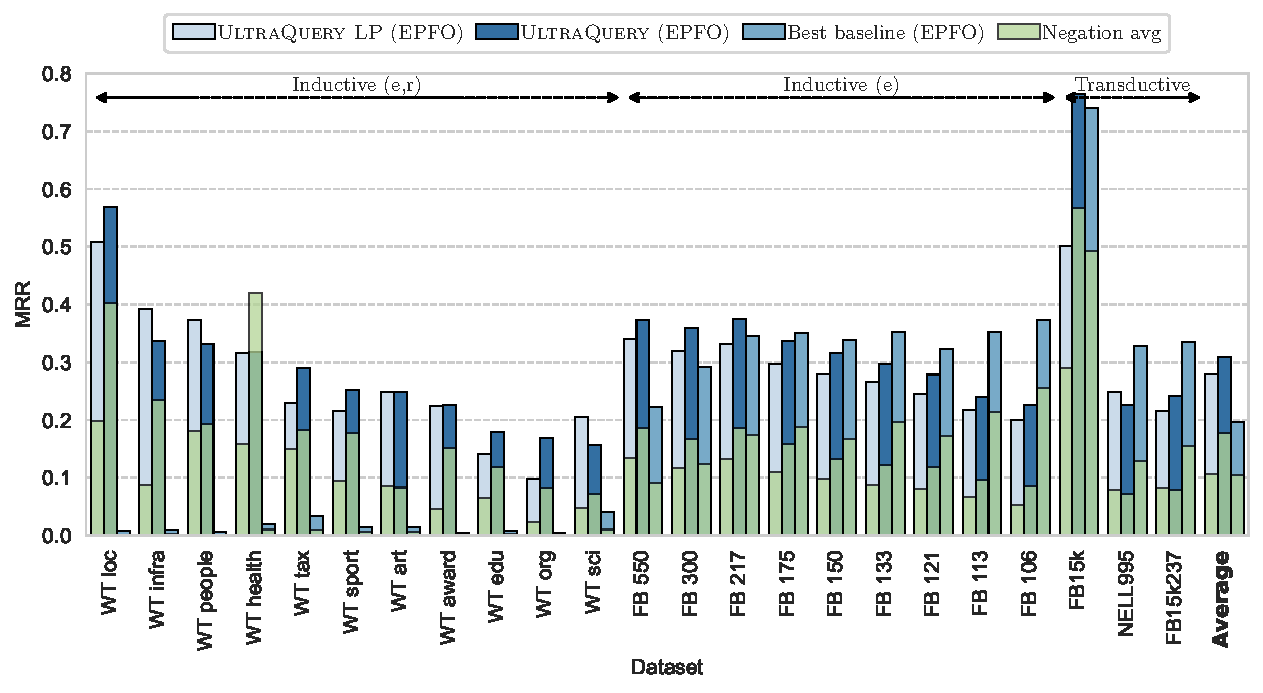
\includegraphics[width=\linewidth]{figs/mainfig1_MRR_pyg.pdf}
    \vskip -0.12 in
    \caption{Zero-shot query answering performance (MRR, higher is better) of a single \method model trained on one FB15k237 queries dataset compared to the best available baselines and ablated \methodlp on 23 datasets. \emph{EPFO} is the average of 9 query types with $(\wedge, \lor)$ operators, \emph{Negation} is the average of 5 query types with the negation operator $(\neg)$. %-- trainable for each transductive and inductive $(e)$ dataset, and the heuristic baseline for newly introduced inductive $(e,r)$ datasets. 
    %\methodlp is an ablated version trained only on \emph{1p} link prediction. 
    On average, a single \method model outperforms the best baselines trained specifically on each dataset. More results are presented in Table~\ref{tab:maintab1} and Appendix~\ref{app:more_results}.
    }
    \label{fig:main_fig1}
\end{figure}

\section{Introduction}
\label{sec:intro}

\begin{wrapfigure}{R}{0.5\textwidth}
\begin{minipage}{0.5\textwidth}
\vspace{-1em}
    %\begin{figure}
        \centering
        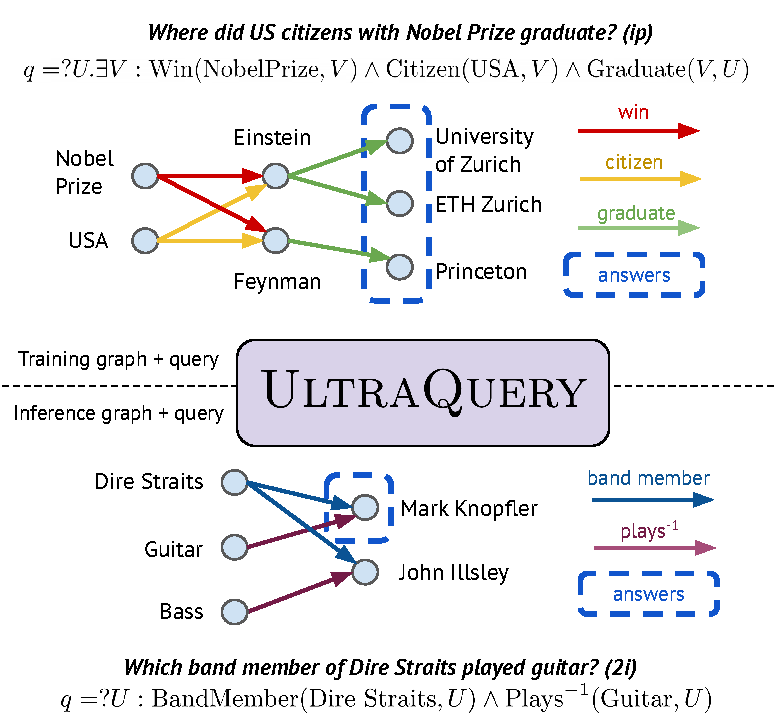
\includegraphics[width=\textwidth]{figs/UltraQuery_Fig1.pdf}
        %\vspace{-2em}
         \vskip -0.1in
        \caption{The inductive logical query answering setup where training and inference graphs (and queries) have different entity and relation vocabularies. We propose a single model (\method) that zero-shot generalizes to query answering % against any unseen
    on any graph with new entity or relation vocabulary at inference time.}
        \label{fig:intro}
    %\end{figure}
    %\vskip -0.2in
    \vspace{-1em}
\end{minipage}
\end{wrapfigure}

Complex logical query answering (\clqa) generalizes simple knowledge graph (KG) completion to more complex, compositional queries with logical operators such as intersection $(\wedge)$, union $(\lor)$, and negation $(\lnot)$.
Such queries are expressed in a subset of first-order logic (FOL) where existentially quantified $(\exists)$ \emph{variables} and given \emph{constants} comprise \emph{relation projections} (or \emph{atoms}), and logical operators combine projections into a logical query (graph pattern). 
A typical example of a logical query~\citep{ren2023ngdb} is presented in \autoref{fig:intro}: $?U.\exists V : \texttt{Win}(\texttt{NobelPrize}, V) \land \texttt{Citizen}(\texttt{USA}, V) \land \texttt{Graduate}(V, U)$ where $\texttt{Win}()$ is a relation projection, $\texttt{NobelPrize}$ is a constant, and $V$ is an existentially quantified variable.




% \begin{figure}[t]
%     \centering
%     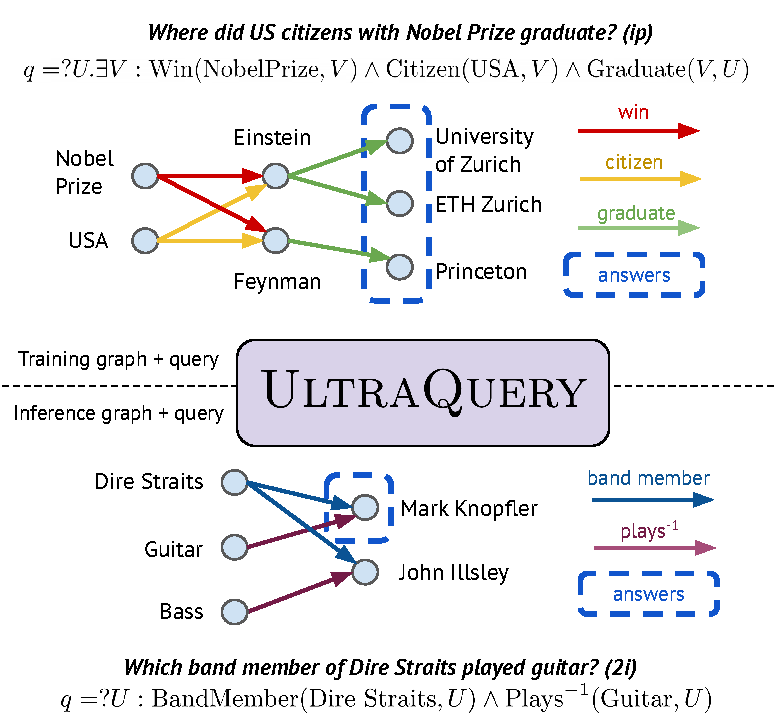
\includegraphics[width=0.5\columnwidth]{figs/UltraQuery_Fig1.pdf}
%     \vskip -0.1in
%     \caption{The inductive logical query answering setup where training and inference graphs (and queries) have different entity and relation vocabularies. We propose a single model (\method) that zero-shot generalizes to query answering % against any unseen
%     on any graph with new entity or relation vocabulary at inference time. \mg{wrapfig it into the first paragraph}}
%     \label{fig:intro}
%     \vskip -0.2in
% \end{figure}

% \clqa assumes that underlying KGs are incomplete such that the projection operator has to predict missing edges and reach the answers unobtainable by simple graph traversal.
Due to the incompleteness of most KGs, these logical queries cannot be directly solved by graph traversal algorithms. Consequently, \clqa methods have to deal with missing edges when modeling the projection operators.
The vast majority of existing \clqa methods~\citep{ren2023ngdb,q2b,betae,cqd,qto} % can only
predict missing edges by learning graph-specific entity and relation embeddings making such approaches transductive and not generalizable to other KGs. 
A few approaches~\citep{gnn_qe,galkin2022,sheaves} are able to generalize query answering to new nodes at inference time but still need a fixed relation vocabulary.

In this work, we focus on the hardest inductive generalization setup where queries and underlying graphs at inference time are completely different from the training graph, \ie, both entities and relations are new.   
Furthermore, we aim at performing \clqa in the \emph{zero-shot} setting with one single model. That is, instead of %training every model on each target dataset,
%adaptively 
finetuning a model on each target dataset,
we seek to design a unified approach that generalizes to any KG and %any complex 
query at inference time.
For example, in \autoref{fig:intro}, the training graph describes academic entities with relations \texttt{Win}, \texttt{Citizen}, \texttt{Graduate}\footnote{We assume the presence of respective inverse relations $\texttt{r}^{-1}$.} whereas the inference graph describes music entities with relations \texttt{Band Member} and \texttt{Plays}. 
The query against the inference graph $?U:\texttt{BandMember}(\texttt{Dire Straits}, U) \wedge \texttt{Plays}^{-1}(\texttt{Guitar}, U)$ involves both new entities 
%(\texttt{Dire Straits}, \texttt{Guitar}) 
and relations 
%(\texttt{Band Member}, \texttt{Plays}) 
and, to the best of our knowledge, cannot be tackled by any existing \clqa method that learns a fixed set of entities or relation embeddings from the training graph.

\textbf{Contributions.} 
Our contributions are two-fold. First, none of the existing \clqa methods can generalize to query answering over new arbitrary KGs with new entities and relations at inference time. 
We bridge this gap by leveraging the recent progress in inductive KG reasoning~\citep{ultra,isdea} and devise \method, the first %\clqa approach 
foundation model for \clqa that generalizes to logical queries on any arbitrary KG with any entity and relation vocabulary in the zero-shot fashion without relying on any external node or edge features. 
%\method follows the blueprint of GNN-QE~\citep{gnn_qe} with the  projection operator parameterized by a graph neural network (GNN) and non-parametric logical operators implemented with fuzzy logics~\citep{vankrieken_fuzzy}.
\method parameterizes the projection operator by an inductive graph neural network (GNN) and implements non-parametric logical operators with fuzzy logics~\citep{vankrieken_fuzzy}.
The pre-trained projection operator~\citep{ultra} does not learn any graph-specific entity nor relation embeddings thanks to the % transferable
generalizable meta-graph representation of relation interactions, and %is therefore zero-shot transferable to any KG.
therefore enables zero-shot generalization to any KG.

% Elaborate more on UltraQuery?

% Experimental evidence
% Furthermore,
Second, in the absence of existing datasets for our inductive generalization setup,
we curate a novel suite of 11 inductive query answering datasets where graphs and queries at inference time  have new entity and relation vocabularies.
Experimentally, we train a single \method model on one dataset and probe on other 22 transductive and inductive datasets.
Averaged across the datasets, a single \method model outperforms by 50\% (relative MRR) the best reported baselines in the literature (often tailored to specific graphs) on both EPFO queries and queries with negation.

% !TEX root = ../main.tex

\section{Background and Analysis}
\label{sec:background}

In this section, we present the notation, setup, and assumptions on which we base the work. Additionally, we conduct an analysis of contrastive \ac{VL} representation learning with multiple captions per image.

\subsection{Preliminaries}
\label{subsec:notation-assumptions}

\header{Notation} We closely follow the notation from \citep{bleeker2023reducing}. 
See Table~\ref{tab:notation} for an overview.
Let $\mathcal{D}$ be a dataset of $N$ image-caption tuples: $\mathcal{D} = \left\{\left(\img{i}, \{\capt{i}{j}\}_{j=1}^{k} \right)\right\}_{i=1}^{N}$. 
Each tuple $i \in N$ contains one image $\img{i}$ and $k$ captions $\capt{i}{j}$, where $1 \leq j \leq k$. 
All captions in tuple $i \in N$ are considered as matching captions w.r.t.\ image $\img{}$ in the tuple $i$.
The latent representation of an image-caption pair from a tuple $i$ is denoted as $\zimg{i}{}$ and $\zcapt{i}{j}$ respectively.
During training, we sample image-caption pairs from the dataset $\mathcal{D}$ and optimize for the evaluation task $T$. 
We include all captions in the dataset once per training epoch, hence, each image is sampled $k$ times.

Given an image $\img{}$, a set of $k$ associated captions $K = \{\capt{}{j}\}_{j=1}^{k}$, and one caption randomly sampled from the set $\capt{}{} \in K$,
we define the following representations:
\begin{enumerate*}[label=(\roman*)]
	\item $\zcaptsuff{}{}$ as \emph{sufficient} representation of the caption $\capt{}{}$ that describes the image $\img{}$;
	\item $\zimgsuff{}$ as representation of the image $\img{}$ \emph{sufficient for the caption} $\capt{}{}$;
	\item $\zminsuff{}$ as representation of the image $\img{}$ that is \emph{minimally sufficient for the caption} $\capt{}{}$; and
	\item $\zoptimal{}{K}$ as representation of the image $\img{}$ that is \emph{optimal for the set of captions} $K$ given the task $T$.
\end{enumerate*}

In addition, we write
$\sct{}$ for a synthetic shortcut,
$S$ for the original shared information, i.e., information that does not contain synthetic shortcuts,
$S^{+}$ for the shared information that includes a synthetic shortcut,
and $R^{+}$ for task-relevant information that contains a synthetic shortcut.

In the context of task relevance, we define $R$ and $\neg R$ as task-relevant and task-irrelevant information, respectively, and $C$ as task-relevant information specific for caption $\capt{}{}$.

\header{Setup} 
We work with a dual-encoder setup, with an image encoder and a caption encoder that do not share parameters. 
The \emph{image encoder} $f_{\theta}(\cdot)$ takes an image $\img{}$ as input and returns its latent representation: $\zimg{}{} :=  f_{\theta}(\img{})$.
Similarly, the \emph{caption encoder} $g_{\phi}(\cdot)$ takes a caption $\capt{}{}$ as input, and encodes the caption into a latent representation: $\zcapt{}{} :=  g_{\phi}(\zcapt{}{})$. 
Both $\zcapt{}{}$ and $\zimg{}{}$ are unit vectors projected into $d$-dimensional multi-modal space: $\zcapt{}{} \in \sR^d$, $\zimg{}{} \in \sR^d$.
For an overview of notation, we refer to Appendix~\ref{appendix:notation}, Table~\ref{tab:notation}.

\header{Assumptions}
Given an image-caption tuple, 
we assume that each caption in the tuple is distinct from the other captions in the tuple.
We also assume that each caption in the tuple contains two types of task-relevant information:
\begin{enumerate*}[label=(\roman*)]
	\item shared information, i.e., information shared with other captions in the same tuple,
	and 
	\item caption-specific information, i.e., information that is not shared with the other captions.
\end{enumerate*}
For simplicity, we base our subsequent analysis on tuples where one image $\img{}{}$ is associated with two captions $\capt{}{A}$ and $\capt{}{B}$: $\left(\img{}, \{\capt{}{A}, \capt{}{B}\} \right)$. 
However, the analysis described in this section can be extended to a case with more than two captions. We treat images and captions as views and define  $\img{}{}$, $\capt{}{A}$, and $\capt{}{B}$ to be random variables of an image and two matching captions, with the joint distribution $p(\img{}{}, \capt{}{A}, \capt{}{B})$.
For more details on assumptions and problem definition, we refer to Appendix~\ref{appendix:problem}.

\subsection{Analysis of Contrastive Vision-Language Representation Learning for Multiple Captions per Image}

\header{InfoMax} We start our analysis of contrastive \ac{VL} representation learning by introducing the InfoMax optimization objective, a typical loss for \ac{VL} representation learning.
The goal of an InfoMax optimization objective, e.g., InfoNCE~\citep{oord2018representation}, is to maximize the \ac{MI} between the latent representations of two views of the same data~\citep{tschannen2020on}. 
Therefore, the optimization objective is equivalent to: $ \max_{f_{\theta}, g_{\phi} } I (\zimg{}{} ; \zcapt{}{} ) $ where $\zimg{} := f_{\theta}(\img{}{})$ and $\zcapt{}{} := g_{\phi}(\capt{}{})$.
%\ay{This definition of task-relevant seems fine for our purposes (and I guess follows prior work), but I think it's really about the dataset rather than the task? It's about the information that exists in a set of existing queries, not about the (many) queries that could reasonably be asked given the task.}


\header{Minimally Sufficient Image Representation} During training, batches of image-caption pairs are sampled. 
The optimization involves maximizing the \ac{MI} between the image representation $\zimg{}{}$ and the matching caption representation $\zcapt{}{}$.
\cite{wang2022rethinking} argue that, since all supervision information for one view (i.e., the image) comes from the other view (i.e., the caption), the representations learned contrastively are approximately minimally sufficient.
Following \citep{tian2020what, wang2022rethinking}, we extend the definition of sufficient representation to \ac{VL} context and define sufficient caption representations, sufficient image representations, and minimally sufficient image representation.

\begin{definition}[Sufficient caption representation]
	\label{def:suff_capt_repr}	
	Given an image $\img{}{}$, and a set of matching captions $\mathcal{C} = \{ \capt{}{A}, \capt{}{B} \}$,
	the representation $\zcaptsuff{}{}$ of caption $\capt{}{} \in \mathcal{C}$ is sufficient for image $\img{}{}$ if, and only if, $I(\zcaptsuff{}{}; \img{}{} ) = I(\capt{}{}; \img{}{})$.
\end{definition}
The sufficient caption representation $\zcaptsuff{}{}$ contains all the information about image $\img{}{}$ in caption $\capt{}{}$.
 
\begin{definition}[Sufficient image representation]
	\label{def:suff_img_repr}		
	Given an image $\img{}{}$, and a set of matching captions $\mathcal{C} = \{ \capt{}{A}, \capt{}{B} \}$,
	the representation $\zimgsuff{}$ of image $\img{}{}$ is sufficient for caption $\capt{}{} \in \mathcal{C}$ if, and only if,  $I(\zimgsuff{}; \capt{}{} ) = I(\img{}{} ; \capt{}{})$.
\end{definition}

Similarly, the sufficient image representation $\zimgsuff{}$ contains all the shared information between an image $\img{}{}$ and a caption $\capt{}{}$. 
% We define it as \emph{pairwise} sufficient because it is defined between a single image-caption pair. 
Note that a sufficient image representation can be sufficient w.r.t.\ multiple captions.

\begin{definition}[Minimally sufficient image representation]
	\label{def:zimgminsuff}		
	Given an image $\img{}{}$, and a set of matching captions $\mathcal{C} = \{ \capt{}{A}, \capt{}{B} \}$,
	the sufficient image representation $\zminsuff{}$ of image $\img{}{}$  is minimally sufficient for caption $\capt{}{} \in \mathcal{C}$ if, and only if, $I(\zminsuff{}; \img{}{}) \leq I(\zimgsuff{}; \img{}{})$, for all $\zimgsuff{}$ that are sufficient.
\end{definition}
Intuitively, $\zminsuff{}$ comprises the smallest amount of information about $\img{}{}$ (while still being sufficient) and, therefore, only contains the information that is shared with caption $\capt{}{}$, i.e., the non-shared information is suppressed.
% Since we assume that everything in the caption is relevant w.r.t.\ the image it describes (see Assumption~\ref{asm:1}), a sufficient caption representation $\zcaptsuff{}{}$ is minimally sufficient.  

\begin{figure*}[t!]
	\centering
	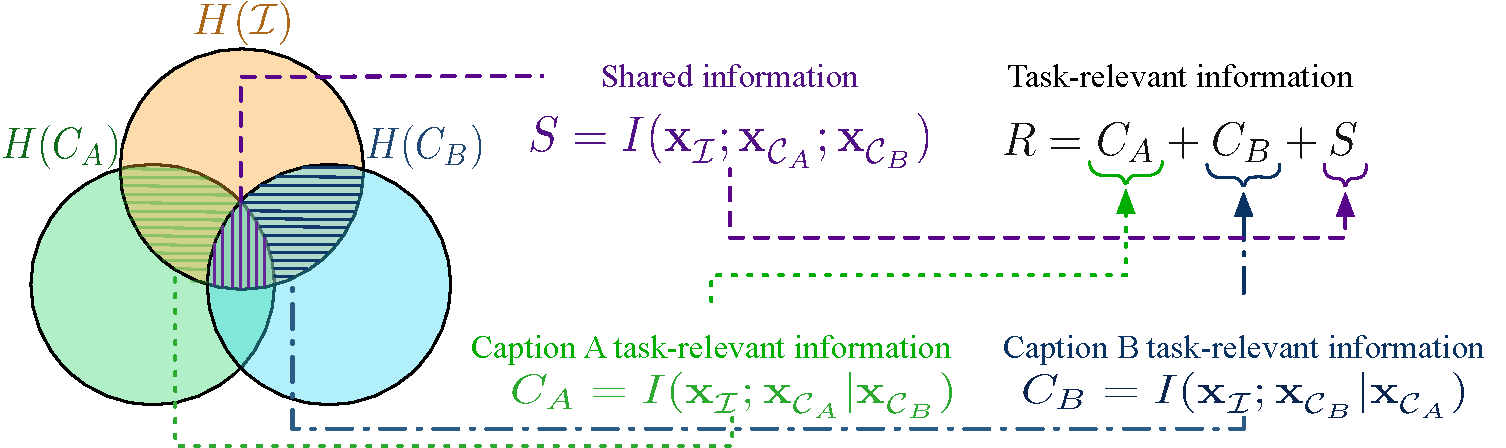
\includegraphics[width=0.85\textwidth]{figures/information-venn-diagram}
	\caption{
		We define $H(\img{}{})$ as image information, $H(\capt{}{A})$ and $H(\capt{}{B})$ as caption information;
		both captions only describe the information depicted in the image and contain shared and caption-specific information.
		We further define
		$C_A = I( \img{}{} ; \capt{}{A} \mid \capt{}{B})$
		and
		$C_B = I( \img{}{} ; \capt{}{B} \mid \capt{}{A})$ as caption-specific information; 
		$S = I(\img{}{} ; \capt{}{A} ; \capt{}{B})$ as shared information;
		$\neg R = H( \img{}{} \mid \capt{}{A} , \capt{}{B} ) $ as task-irrelevant information;
		$R = C_A + C_B + S$ as task-relevant information.
	}
	\label{fig:venn}
\end{figure*} 

\header{Task-Optimal Image Representation} The definition of task-optimal image representation is based on the notion of task-relevant information. 
In the context of \ac{VL} representation learning with multiple captions per image, we define task-relevant information as all information described by the matching captions. That includes both caption-specific and shared information.
Consequently, task-optimal image representation is image representation that is sufficient w.r.t. all matching captions.

Formally, following assumptions from Appendix~\ref{app:assumptions}, we define task-relevant information $R$ as all the information described by the matching captions. The task-relevant information can be expressed as follows:
%
\begin{equation}
\begin{split}
	\underbrace{R}_{\substack{\text{Task-relevant}\\ \text{information}}} & =
	\underbrace{H(\img{}{} )}_{\substack{\text{Image}\\ \text{information}}}
	- \underbrace{H(\img{}{} \mid \capt{}{A} , \capt{}{B})}_{\substack{\text{Task-irrelevant}\\ \text{information}}}
	\\
	& = 
	\underbrace{I( \img{}{} ; \capt{}{A} \mid \capt{}{B})}_{\substack{\text{$C_{A}$-specific}\\ \text{task-relevant information}}}
	+
	\underbrace{I( \img{}{} ; \capt{}{B} \mid \capt{}{A})}_{\substack{\text{$C_{B}$-specific}\\ \text{task-relevant information}}}
	+
	\underbrace{I(\img{}{} ; \capt{}{A};\capt{}{B})}_{\substack{\text{Shared}\\ \text{information}}}.
\end{split}	
	\label{eq:task_relevant}
\end{equation}
%
Similarly, task-irrelevant information $\neg R$ is the image information not described by the captions. Figure~\ref{fig:venn} illustrates both definitions.

The multi-view assumption states that task-relevant information for downstream tasks comes from the information shared between views~\citep{shwartz2023compress}.  
However, in the case of \ac{VL} representation learning with multiple captions per image, task-relevant information $R$ includes both shared information $S$, and caption-specific information $C_A$ and $C_B$ (Eq.~\ref{eq:task_relevant}).

\begin{definition}[Task-optimal image representation]
	\label{def:opt_z}	
	Given an image $\img{}{}$, and a set of matching captions $\mathcal{C} = \{ \capt{}{A}, \capt{}{B} \}$, 
	the representation $\zoptimal{}{\mathcal{C}}$ is task-optimal image representation for all matching captions if, and only if, $I(\zoptimal{}{\mathcal{C}}; \capt{}{}) = I(\img{}{}; \capt{}{})$, for all $\capt{}{} \in \mathcal{C}$.
\end{definition}
In other words, task-optimal image representations contain all the information that the image shares with the matching captions. 
Hence, a task-optimal image representation is sufficient w.r.t.\ all matching captions. 
The information contained in the task-optimal image representation includes both shared and caption-specific information.
Therefore, a task-optimal image representation can never be a minimally sufficient image representation w.r.t.\ to a specific caption.

\begin{thm}{1}[Suboptimality of contrastive learning with multiple captions per image]
	\label{thm:suboptimality-main}	
	Given an image $\img{}{}$, a set of matching captions $\mathcal{C} = \{ \capt{}{A}, \capt{}{B} \}$, and a contrastive learning loss function $\infonce{}$ that optimizes for task $T$, 
	image representations learned during contrastive learning will be minimally sufficient and will never be task-optimal image representations.
\end{thm}

The proof is provided in Appendix~\ref{app:analysis-of-contrastive}.
Rephrasing Theorem~\ref{thm:suboptimality-main}, given an image and two captions that form two image-caption pairs, $(\img{}{}, \capt{}{A})$ and $(\img{}{}, \capt{}{B})$, and assuming that contrastive loss optimizes the image encoder to be minimally sufficient w.r.t.\ to caption $\capt{}{A}$ during a training step, all task-relevant information $C_{B}$ specific to caption $\capt{}{B}$ will be suppressed in $\zimg{}{}$. Hence, the resulting image representation will not be optimal for the task $T$.

Theorem~\ref{thm:suboptimality-main} indicates a discrepancy between minimally sufficient representations learned during contrastive training with the InfoNCE loss and the task-optimal image representations in the context of learning \ac{VL} representations with multiple captions per image.
Although the InfoMax loss does not have an explicit constraint to compress information, prior work indicates that feature suppression is happening \citep{shwartz2023compress, robinson2021can}. 
Hence, we question if contrastive loss can be used to learn task-optimal image representations in the context of multiple captions per image.

Furthermore, Theorem~\ref{thm:suboptimality-main} implies that in the context of contrastive \ac{VL} representation learning with multiple captions per image, the minimally sufficient representation, which discards non-shared information, is not the same as the task-optimal representation that comprises both caption-specific and shared information.  
This suggests that the features learned during contrastive learning might be shortcuts, i.e., easy-to-detect discriminatory features that minimize the contrastive optimization objective but are not necessarily sufficient for solving the evaluation task.
To examine this problem, we introduce a synthetic shortcuts framework that allows us to investigate the problem of suboptimality of contrastive learning with multiple captions per image in a controlled way.

% !TEX root = ../main.tex

\section{Synthetic Shortcuts to Control Shared Information}
\label{eval:method}

In Section~\ref{sec:background} we show the suboptimality of the contrastive InfoNCE loss with multiple captions per image.
In the case of real-world \ac{VL} datasets with multiple captions per image, there are no annotations that indicate the information shared between the image and captions and the information specific to each caption.
Hence, we cannot directly measure how much of the shared and unique information is captured by the representations.

\begin{wrapfigure}[17]{R}{0.4\textwidth}
	\centering
	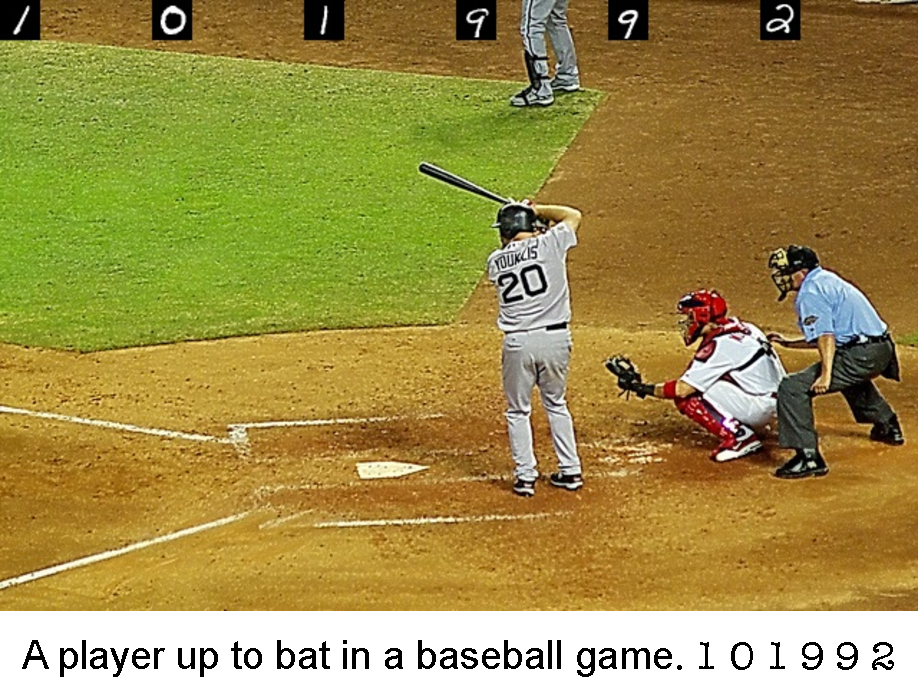
\includegraphics[width=0.4\textwidth]{figures/shortcut-example}
	\caption{An image-caption pair from the MS-COCO dataset with a shortcut added to both the image and the caption.}
	\label{fig:shortcut-example}
\end{wrapfigure}

\header{Synthetic Shortcuts}
In this section, we introduce the \textit{\acf{SVL}} training and evaluation framework.
We denote the \textit{synthetic shortcuts for image-caption data} as $\sct{}$.
The purpose of the framework is to introduce additional and easily identifiable information shared between an image and the matching captions that lacks any semantic meaning. 
The shortcuts we use in this work are represented as numbers that we add to images and captions.
For images, we add the shortcut number by adding MNIST images as an overlay to the original images.
For captions, we append the numbers of the shortcut as extra tokens at the end of the caption.

Figure~\ref{fig:shortcut-example} illustrates an example of an image-caption pair with an added shortcut.
The example contains an image with the caption: `A player up to bat in a baseball game. 1 0 1 9 9 2.'
Here, `1 0 1 9 9 2' is a shortcut added to both the image and the caption. 
For the image modality, we add the shortcut by overlaying MNIST images at the top of the original image.
For the text modality, we append the shortcut as additional tokens at the end of the caption.
This identifier provides an additional link between the image and the caption without carrying any semantic meaning related to their content. 
Additional examples are shown in Figure~\ref{fig:shortcut_examples}.

If contrastive losses learn task-optimal representations, then the presence of synthetic shortcuts should not negatively impact the evaluation performance, since synthetic shortcuts represent additional information and the remaining task-relevant information is intact.
By incorporating synthetic shortcuts into the image-caption dataset, the shared information would include the information that was originally shared and the synthetic shortcut:
$S^{+} = S + \sct{}$.
Hence, the task-relevant information would comprise caption-specific information that was originally shared and a synthetic shortcut:
$R^{+} = C_A + C_B + S + \sct{}$. 
If injecting a synthetic shortcut influences the performance negatively, we can conclude that by learning to represent a synthetic shortcut the model suppresses other task-relevant information in favor of the shortcut, hence the representation is not task-optimal.
The setup is inspired by the ``datasets with explicit and controllable competing features,'' introduced by \cite{chen2021intriguing}, but we adapt this setup to the \ac{VL} scenario.

For experiments, we use the \ac{Flickr30k} and \ac{MS-COCO} image-caption datasets, that consist of image-caption tuples, each image is associated with five captions.
During training, we sample a batch of image-caption pairs $\mathcal{B} = \{(\img{i}, \capt{i}{j}), \dots\}_{i=1}^{|\mathcal{B}|}$, from dataset $\mathcal{D}$, and apply shortcut sampling.
We inject the shortcuts in a manner that preserves the original information of the images and captions. 
Furthermore, we append the shortcut after applying data augmentations to ensure that the shortcut is present in both the images and captions (i.e., the shortcut is not augmented away).
We refer to Figure~\ref{fig:shortcut_examples} for some examples.
The training, evaluation, and implementation details of the shortcut sampling are provided in Appendix~\ref{app:experimental-shortcutsampling}.

We define the following experimental setups:
\begin{enumerate}[label=\Roman*]
	\item \emph{No shortcuts}: As a baseline, we fine-tune a pre-trained CLIP~\citep{radford2021learning} and train VSE++~\citep{faghri2018improving} from scratch on \ac{Flickr30k} and \ac{MS-COCO}, without using any shortcuts. 
	The experimental setup for training both models is provided in Appendix~\ref{app:experimental-models} and \ref{app:experimental-training}. 
	The goal of this setup is to show the retrieval evaluation performance without adding any shortcuts for both a large-scale pre-trained foundation model and a small-scale model trained from scratch.
	\item \emph{Unique shortcuts}: We add a unique shortcut to each image-caption tuple $i \in\mathcal{D}$ in the dataset. 
	In this setup, each image caption pair can be uniquely matched during training by only detecting the shortcut. 
	For each tuple $i \in \mathcal{D}$, we use the number $i$ as the number of the shortcut we inject to the image and captions in the tuple.
	If the contrastive loss learns task-optimal representations, the downstream evaluation performance should not decrease when training with unique shortcuts.
	\item \emph{Unique shortcuts on only one modality}: To show that the shortcuts do not interfere with the original task-relevant information ($S, C_A$, and $C_B$) of the images and captions, we create a dataset with only shortcuts on either the image or caption modality. Therefore, the shortcut cannot be used by the encoders to match an image-caption pair. 
	Hence, we expect the encoders to ignore the shortcuts and extract the features from the original data similar to the features learned by the baseline models in experimental setup \rom{1}.
	\item \emph{N bits of shortcuts}: In this setup, for each image-caption pair in the training batch $\mathcal{B}$, we randomly sample a shortcut number from the range $[0, 2^{n}]$, where $n$ is the number of bits.
	The higher the value of $n$, the more image-caption pairs in the training batch will have by expectation a unique shortcut, and, the less the model has to rely on $S$ and the remaining task-relevant information to solve the contrastive objective. 
	The goal of this setup is to show that, the more unique (shortcut) information is present per sample in the batch, the less contrastive models rely on the remaining task-relevant information.
\end{enumerate}
 It should be noted that the shortcuts we add are independent of the image-caption pairs. 
 However, the goal of the \ac{SVL} framework is to measure the effect of the presence of additional easy-to-detect shared information on the learned representations. 

 \header{Evaluation Method}
To show the effect of the injected shortcuts on retrieval evaluation performance, we evaluate both with and without adding the shortcuts during evaluation.
When training with unique shortcuts, we add a unique shortcut to each tuple in the test set as well.
When training with shortcuts on either one of the two modalities, we only evaluate without shortcuts to show that training with shortcuts on one modality does not influence performance.
When training with $n$ bits of shortcuts, we add the shortcut $\mod(i, n)$ (modulo) to each tuple $i$ in the evaluation set, to make sure we use the same number of shortcuts during evaluation as during training.
To facilitate the reproducibility and support further research, we provide the code with our paper.\footnote{ \url{https://github.com/MauritsBleeker/svl-framework}}

% !TEX root = ../main.tex
\section{Synthetic Shortcuts and their Impact on Learned Representations and Evaluation Performance}
\label{eval:results}

\begin{figure}[t!]
\centering
\begin{subfigure}[b]{\textwidth}
	\includegraphics[width=1\linewidth]{figures/results/CLIP-f30k-coco-shortcut-eval-linear.pdf}
	\vspace*{-6mm}
	\caption{Evaluation results for the CLIP model when using different shortcut sampling setups. }
	\label{fig:results_clip}
\end{subfigure}

\vspace*{4mm}
\begin{subfigure}[b]{\textwidth}
	\includegraphics[width=1\linewidth]{figures/results/VSE-f30k-coco-shortcut-eval-linear.pdf}
	\vspace*{-6mm}
	\caption{Evaluation results for the VSE++ model when using different shortcut sampling setups. }
	\label{fig:results_vse} 
\end{subfigure}
\caption{Effect of synthetic shortcuts on CLIP and VSE++ performance on \ac{ICR} task.
The dotted line represents the maximum achievable recall sum, while the dashed line for CLIP indicates its zero-shot evaluation performance
(Best viewed in color.)}
\label{fig:shortcuts_results}
\end{figure}

\subsection{Findings}
First, we train and evaluate both a CLIP and VSE++  without shortcuts on the \ac{Flickr30k} and \ac{MS-COCO} dataset for the image-caption retrieval task as a baseline. 
We use the recall sum (i.e., the sum of $R@1, R@5$, and $R@10$ for both \ac{i2t} and \ac{t2i} retrieval) as evaluation metric (see Appendix~\ref{appendix:task} for the evaluation task description). 
We visualize the results in~Figure~\ref{fig:shortcuts_results}.
The dotted line (in Figure~\ref{fig:results_clip} and~\ref{fig:results_vse}) indicates the maximum evaluation score (i.e., 600). 
For CLIP, we also provide the zero-shot performance of the model, indicated by the dashed line in Figure~\ref{fig:results_clip}. 
When referring to specific results in~Figure~\ref{fig:shortcuts_results}, we use the color of the corresponding bar and legend key in brackets in the text.

Based on Figure~\ref{fig:shortcuts_results}, we draw the following conclusions: 
\begin{enumerate}[label=\Roman*]
	\item When training CLIP and VSE++ with only shortcuts on either the caption modality (in Figure~\ref{fig:shortcuts_results}, the corresponding bar/legend box is colored \caponly) or on the image modality~(\imgonly, in Figure~\ref{fig:shortcuts_results}), we do not observe a drop in evaluation scores for CLIP compared to the baseline model (\baseline, in Figure~\ref{fig:results_clip}).
	For VSE++ we only observe a slight drop in evaluation score when training with shortcuts on the caption modality (again \caponly, mainly for \ac{MS-COCO}, in Figure~\ref{fig:results_vse}).  
	Therefore, we conclude that the synthetic shortcuts do not interfere with the original shared information $S$ or other task-relevant information.
	
	\item When training the models with \textit{unique shortcuts}, we observe for both CLIP and VSE++ that when evaluating with shortcuts~(\uswith, in Figure~\ref{fig:shortcuts_results}), the models obtain a perfect evaluation score. 
	When evaluating without shortcuts (\uswithout, in Figure~\ref{fig:shortcuts_results}) the evaluation score for VSE++ drops to zero and for CLIP below the zero-shot performance. 
	We conclude that with unique shortcuts:
	\begin{enumerate*}[label=(\roman*)]
		\item both CLIP and VSE++ fully rely on the shortcuts to solve the evaluation task,
		\item VSE++ has not learned any other shared or task-relevant information other than the shortcuts (since it is trained from scratch, only detecting the shortcuts is sufficient to minimize the contrastive loss), and 
		\item fine-tuned CLIP has suppressed original features from the zero-shot model in favor of the shortcuts.	
	\end{enumerate*}
	
	\item When training the models with \textit{N bits of shortcuts}, we observe for both CLIP and VSE++ that the larger the number of bits we use during training and when evaluating without shortcuts~(\bswithout, in Figure~\ref{fig:shortcuts_results}), the bigger the drop in evaluation performance. 
	When we evaluate with shortcuts~(\mbox{\bswith,} in Figure~\ref{fig:shortcuts_results}), the evaluation performance improves as we use more bits compared to the baseline without shortcuts~\baseline, in Figure~\ref{fig:shortcuts_results}). 
	For VSE++, evaluating without shortcuts~(\bswithout, in Figure~\ref{fig:results_vse}) results in a drop to zero when having a large number of bits.
	 For CLIP, the evaluation performance drops below the zero-shot performance. 
	 If we train with 0 bits of shortcuts (i.e., the shortcut is a constant) we do not observe any drop or increase in evaluation scores for CLIP.
\end{enumerate}

\subsection{Upshot}
Given the findings based on Figure~\ref{fig:shortcuts_results} we conclude that a contrastive loss (i.e., InfoNCE) mainly learns the easy-to-detect minimal shared features among image-caption pairs that are sufficient to minimize the contrastive objective while suppressing the remaining shared and/or task-relevant information.  
If contrastive losses are sufficient to learn task-optimal representations for image-caption matching, these shortcuts should not adversely impact the evaluation performance.
Moreover, if the contrastive loss would only learn features that are shared among the image and all captions (i.e, $S$), we should not observe a drop in performance to 0 for the VSE++ model when training with unique shortcuts, since there is still a lot of task-relevant information present in $S$.
Especially in a training setup where a model is trained from scratch or fine-tuned on small datasets, the easy-to-detect features are likely not equivalent to all task-relevant information in the images and captions.
Hence, we conclude that contrastive loss itself is not sufficient to learn task-optimal representations of the images (and sufficient representations of captions) and that it only learns the minimal easy-to-detect features that are needed to minimize the contrastive objective.


% !TEX root = ../main.tex

\section{Reducing Shortcut Learning}
\label{sec:reducing_shortcut_solution}

In the earlier section, we have demonstrated that contrastive loss mainly relies on the minimal, easy-to-detect features shared among image-caption pairs while suppressing remaining task-relevant information.
In this section, we describe two methods that help to reduce shortcut learning for contrastive learning on our \ac{SVL} framework: \Acl{LTD}~\citep{bleeker2023reducing} and  \acl{IFM}~\citep{robinson2021can}. 

\subsection{Latent Target Decoding}  

\Acf{LTD}~\citep{bleeker2023reducing} is a method to reduce predictive feature suppression (i.e., shortcut learning) for resource-constrained contrastive image-caption matching. 
The contrastive objective (i.e., InfoNCE)  is combined with an additional reconstruction loss, which reconstructs the input caption from the latent representation of the caption $\zcapt{i}{j}$. 
We refer to Appendix~\ref{app:ltd} for the mathematical definition of \ac{LTD}.
Instead of reconstructing the tokens of the input caption in an auto-regressive manner (i.e., auto-encoding), the caption is reconstructed non-auto-regressively, by mapping the caption representation into the latent space of a \acl{SBERT}~\citep{reimersers2019sentence, song2020mpnet} and minimizing the distance (i.e., reconstructing) between the reconstruction and the \acl{SBERT} representation of the caption $\capt{i}{j}$. 
The assumption is that the \emph{target} generated by the \acl{SBERT} model contains all task-relevant information in the caption. 
Hence, by correctly mapping the latent caption representation $\zcapt{i}{j}$ into the latent space of \acl{SBERT}, the caption encoder cannot suppress any task-relevant information or rely on shortcut solutions. 
\ac{LTD} is implemented both as a dual-loss objective (i.e., the contrastive loss and \ac{LTD} are added up) and as an optimization constraint while minimizing the InfoNCE loss, by implementing the loss as a Lagrange multiplier. For the mathematical definition of \ac{LTD}, we refer to Appendix~\ref{app:ltd}.

\header{Experimental Setup} We use the \ac{LTD} implementation and set-up similar to \citet{bleeker2023reducing}. 
We train both CLIP and VSE++ with \ac{LTD}, implemented as either dual loss or an optimization constraint.
When implementing \ac{LTD} as a constraint, we try $\eta \in \{0.01, 0.05, 0.1, 0.15, 0.2, 0.25, 0.3\}$ as bound values.
Similar to \cite{bleeker2023reducing}, when implementing \ac{LTD} as a dual loss, we use $\beta=1$ as balancing parameters.   
We train both with and without unique shortcuts.  
We do this to show 
\begin{enumerate*}[label=(\roman*)]
	\item what the performance improvement is compared to using only InfoNCE, and 
	\item to what degree \ac{LTD} prevents full collapse to shortcut features.
\end{enumerate*}
For each model and dataset, we take the training setup that results in the highest performance on the validation set.

\subsection{Implicit Feature Modification} 
\Acf{IFM}~\citep{robinson2021can} is a method, originally introduced in the context of representation learning for images,
that applies perturbations to logits used for guiding contrastive models. 
\ac{IFM} perpetuates features that the encoders use during a training step to discriminate between positive and negative samples. 
By doing so, \ac{IFM} alters the features that are currently used to solve the discrimination task, to avoid the InfoNCE loss to learn shortcut solutions.  
How much of the features are removed, is defined by a perturbation budget $\epsilon$.
\ac{IFM} is implemented as a dual loss in combination with the InfoNCE loss. 
For the mathematical definition of \ac{IFM}, we refer to Appendix~\ref{app:ifm}.

\header{Experimental Setup}
We apply a similar experimental set-up for \ac{IFM} as for \ac{LTD}.
We apply \ac{IFM} both to CLIP and to VSE++, both with and without unique shortcuts.
Similar to \citep{robinson2021can}, we try different perturbation budgets $\epsilon$, we try $\epsilon \in \{0.05, 0.1, 0.2, 0.5, 1\}$.
In line with the \ac{LTD} setup, we take the training setup that results in the highest performance on the validation set.

\subsection{Method Comparison}
Both \ac{LTD} and \ac{IFM} aim to mitigate shortcut learning through different approaches.
\ac{LTD} aims to learn all task-relevant information by reconstructing the input captions.
In contrast, \ac{IFM} perturbs the discriminative features in the latent space of the encoder and does not rely on a reconstruction objective.
Overall, both methods represent distinct strategies for improving the robustness and generalization capabilities of \ac{VL} representation learning.

In the following section, we present experimental results with \ac{LTD} and \ac{IFM}, providing insight into their effectiveness in mitigating shortcut learning.

% !TEX root = ../main.tex

\section{Experimental Results}
\label{sec:shorcut_results}

\subsection{Does Latent Target Decoding Reduce Shortcut Learning?}

In Table~\ref{tab:ltd} we summarize the effect of \ac{LTD} on reducing shortcut learning. 

For CLIP, for both the \ac{Flickr30k} and \ac{MS-COCO} dataset, we do not observe an increase in recall scores when fine-tuning with $\ltd{}$ compared to models that are only fine-tuned with $\infonce{}$. 
LTD has originally been proposed for resource-constrained \ac{VL} models. 
We argue that the additional features that LTD can extract are either already present in the pre-trained CLIP model, or not relevant for the evaluation task. 
However, when fine-tuning with $\ltd{}$ and in the presence of shortcuts in the training data, degradation in recall scores is significantly lower than when fine-tuned only with the $\infonce{}$. 
This shows that LTD can reduce the suppression of features in favor of the shortcut features when fine-tuning large-scale \ac{VL} models. 

% !TEX root = ../../main.tex

\begin{table*}[t!]
	\centering
	\caption{Mean and variance (over three training runs) recall@$k$ evaluation scores for the \ac{Flickr30k} and \ac{MS-COCO} datasets for image-to-text and text-to-image retrieval. 
		We train with two loss functions: $\infonce{}$ and $\ltd{}$. 
		We train either with (\checkmark) or without (\xmark) shortcuts. 
		For the model trained with $\ltd{}$, we provide the hyper-parameters of the best-performing model. $\eta$ indicates that the best-performing model uses LTD implemented as an optimization constraint with bound $\eta$. $\beta$ indicates that the best-performing model uses LTD implemented as a dual-loss with $\beta=1$.
		}
	\setlength{\tabcolsep}{1.5pt}
	\resizebox{\textwidth}{!}{%
	\begin{tabular}{@{\extracolsep{1pt}}l @{} c r@{$_\pm$}l r@{$_\pm$}l r@{$_\pm$}l r@{$_\pm$}l r@{$_\pm$}l r@{$_\pm$}l r@{$_\pm$}l}
		\toprule
		& & \multicolumn{6}{c}{\textit{i2t}} & \multicolumn{6}{c}{\textit{t2i}} & \multicolumn{2}{c}{ \ } \\
		\cmidrule(r){3-8} \cmidrule(r){9-14} \cmidrule{15-16}
		Loss & $\sct{}$ & \multicolumn{2}{c}{R@1}  & \multicolumn{2}{c}{R@5}  & \multicolumn{2}{c}{R@10} & \multicolumn{2}{c}{R@1}  & \multicolumn{2}{c}{R@5}  & \multicolumn{2}{c}{R@10}  & \multicolumn{2}{c}{rsum} \\ 
		\midrule
		\multicolumn{16}{c}{Flickr30k}\\
		\midrule
		& & \multicolumn{14}{c}{CLIP}                                                   \\
		\cmidrule{3-16}
		$\infonce{}$     &   \xmark &   ${86.9}$ & $_{0.1}$ & $\textbf{97.4}$ & $_{0.1}$ & $\textbf{99.0}$ & $_{0.0}$ & ${72.4}$ & $_{0.1}$ & $\textbf{92.1}$ & $_{0.0}$ & $\textbf{95.8}$ & $_{0.0}$ & ${543.5}$ & $_{1.1}$  \\
		$\ltd{}$, $\beta=1$ &  \xmark & ${86.5}$ & $_{0.6}$-- & ${97.1}$ & $_{0.0}\negative$ & ${98.5}$ & $_{0.0}\negative$& ${72.4}$ & $_{0.0}$-- & ${92.3}$ & $_{0.0}\negative$ & ${95.9}$ & $_{0.0}\negative$&  ${542.8}$ & $_{0.8}$--\\
		\cmidrule(r){3-16}
		$\infonce{}$  &  \checkmark  &  ${57.2}$ & $_{8.3}$ & ${84.0}$ & $_{4.8}$ & ${91.0}$ & $_{1.9}$ & ${44.9}$ & $_{4.5}$ & ${74.9}$ & $_{6.0}$ & ${84.2}$ & $_{2.5}$ & ${436.2}$ & $_{145.0}$  \\
		$\ltd{}$,  $\beta=1$ & \checkmark  & $\textbf{64.0}$ & $_{1.3}\positive$ & $\textbf{87.8}$ & $_{0.9}\positive$ & $\textbf{93.2}$ & $_{0.8}\positive$ & $\textbf{50.7}$ & $_{0.6}\positive$ & $\textbf{79.8}$ & $_{0.7}\positive$ & $\textbf{88.1}$ & $_{0.5}\positive$ & $\textbf{463.6}$ & $_{17.3}\positive$ \\
		\cmidrule{3-16}
		&  & \multicolumn{14}{c}{VSE++} \\
		\cmidrule{3-16}
		$\infonce{}$  & \xmark &  ${52.6}$ &$_{1.1}$ & ${79.8}$ & $_{0.1}$ & ${87.8}$ & $_{0.1}$ & ${39.5}$ & $_{0.3}$ & ${69.8}$ & $_{0.0}$ & ${79.4}$ & $_{0.1}$ & ${409.0}$ & $_{4.0}$\\
		$\ltd{}$, $\eta=0.2$ & \xmark & $\textbf{54.1}$ & $_{0.1}\positive$ & $\textbf{81.1}$ & $_{0.8}\positive$ & $\textbf{88.6}$ & $_{0.1}\positive$ & $\textbf{42.5}$ & $_{0.0}\positive$ & $\textbf{71.9}$ & $_{0.1}\positive$ & $\textbf{81.3}$ & $_{0.0}\positive$ & $\textbf{419.6}$ & $_{0.1}\positive$  \\
		\cmidrule(r){3-16}
		$\infonce{}$  &  \checkmark  &  ${0.1}$ & $_{0.0}$ & ${0.6}$ & $_{0.1}$ & ${1.1}$ & $_{0.1}$ & ${0.1}$ & $_{0.0}$ & ${0.5}$ & $_{0.0}$ & ${1.0}$ & $_{0.0}$ & ${3.4}$ & $_{0.6}$ \\
		$\ltd{}$, $\eta=0.05$ & \checkmark  &  $\textbf{24.7}$&$_{0.5}\positive$ & $\textbf{51.8}$ & $_{0.7}\positive$ & $\textbf{65.6}$ & $_{1.4}\positive$ & $\textbf{20.7}$ & $_{1.0}\positive$ & $\textbf{49.2}$ & $_{0.6}\positive$ & $\textbf{62.6}$ & $_{1.2}\positive$ & $\textbf{274.6}$ & $_{4.6}\positive$ \\
		\midrule
		\multicolumn{16}{c}{\ac{MS-COCO}}\\
		\midrule
		& & \multicolumn{14}{c}{CLIP}\\
		\cmidrule(r){3-16} 
		$\infonce{}$     &   \xmark & ${63.8}$ & $_{0.3}$ & ${86.1}$ & $_{0.2}$ & ${92.3}$ & $_{0.0}$ & ${46.3}$ & $_{0.3}$ & ${74.8}$ & $_{0.1}$ & ${84.1}$ & $_{0.2}$ & ${447.5}$ & $_{0.5}$  \\
		$\ltd{}$, $\beta=1$ &  \xmark & ${63.8}$ & $_{0.0}$-- & ${86.1}$ & $_{0.0}$-- & ${92.3}$ & $_{0.0}$-- & ${46.3}$ & $_{0.0}$-- & ${74.7}$ & $_{0.0}$-- & ${84.1}$ & $_{0.0}$-- & ${447.4}$ & $_{0.0}$-- \\
		\cmidrule(r){3-16}
		$\infonce{}$  &  \checkmark & ${13.6}$ & $_{0.9}$ & ${31.5}$ & $_{2.4}$& ${42.2}$ & $_{3.7}$ & ${\phantom{0}7.3}$ & $_{0.6}$ & ${22.1}$ & $_{1.0}$ & ${32.7}$ & $_{1.7}$ & ${149.4}$ & $_{32.7}$  \\
		$\ltd{}$, $\beta=1$ & \checkmark &  $\textbf{18.9}$ & $_{0.1}\positive$ & $\textbf{41.8}$ & $_{0.1}\positive$ & $\textbf{54.1}$ & $_{0.1}\positive$ & $\textbf{16.5}$ & $_{0.0}\positive$ & $\textbf{39.4}$ & $_{0.0}\positive$ & $\textbf{52.6}$ & $_{0.1}\positive$ & $\textbf{223.4}$ & $_{0.2}\positive$ \\
		\cmidrule{3-16} 
		&  & \multicolumn{14}{c}{VSE++} \\
		\cmidrule{3-16} 
		$\infonce{}$  & \xmark  & ${42.2}$ & $_{0.1}$ & ${72.7}$ & $_{0.1}$ & ${83.2}$ & $_{0.1}$ & ${30.9}$ & $_{0.0}$ & ${61.2}$ & $_{0.1}$& ${73.5}$ & $_{0.1}$ & ${363.8}$ & $_{2.3}$ \\
		$\ltd{}$, $\eta=0.1$ & \xmark & $\textbf{43.6}$ & $_{0.1}\positive$ & $\textbf{73.5}$ & $_{0.0}\positive$ & $\textbf{83.7}$ & $_{0.0}\positive$ & $\textbf{32.4}$ & $_{0.1}\positive$ & $\textbf{62.5}$ & $_{0.0}\positive$ & $\textbf{74.7}$ & $_{0.0}$ & $\textbf{370.5}$ & $_{0.1}\positive$   \\
		\cmidrule(r){3-16}
		$\infonce{}$    &  \checkmark & ${0.0}$ & $_{0.0}$ & ${0.1}$ & $_{0.0}$ & ${0.2}$ & $_{0.0}$ & ${\phantom{0}0.0}$ & $_{0.0}$ & ${\phantom{0}0.1}$ & $_{0.0}$ & ${\phantom{0}0.2}$ & $_{0.0}$ & ${\phantom{00}0.7}$ & $_{0.0}$ \\ 
		$\ltd{}$, $\eta=0.01$ & \checkmark & $\textbf{3.9}$ & $_{0.0}\positive$ & $\textbf{13.7}$ & $_{0.6}\positive$ & $\textbf{21.6}$ & $_{0.9}\positive$ & $\textbf{\phantom{0}3.1}$ & $_{0.2}\positive$ & $\textbf{11.0}$ & $_{1.6}\positive$ & $\textbf{18.1}$ & $_{3.0}\positive$ & $\textbf{\phantom{0}71.3}$ & $_{3.6}\positive$  \\
		\bottomrule
	\end{tabular}%
	}
\label{tab:ltd}
\end{table*}

Across the board, VSE++ models trained with the $\ltd{}$ loss consistently outperform the $\infonce{}$ loss, both for \ac{i2t} and \ac{t2i} retrieval and both when trained either with or without shortcuts, as indicated by higher recall@$k$ scores; this is consistent with the findings presented in \citep{bleeker2023reducing}).
For both the \ac{Flickr30k} and \ac{MS-COCO} dataset, when trained with the $\infonce{}$ and with shortcuts present in the training data, the model performance collapses to around 0 in the absence of shortcuts (as we have seen in Section~\ref{eval:results}). 
However, when we train with shortcuts in the training data and with $\ltd{}$, we observe, for both \ac{Flickr30k} and \ac{MS-COCO}, a significant gain in performance. 
The performance improvement is bigger for \ac{Flickr30k} than for \ac{MS-COCO}.
In general, the recall scores are still significantly lower than training without shortcuts, however, the models do not solely rely on the shortcuts anymore to minimize the contrastive loss and are able during evaluation (in the absence of shortcuts) to still correctly match image-caption pairs with each other.
The results in Table~\ref{tab:ltd} show that LTD is able, in the presence of shortcuts in the training data, to guide (small-scale) \ac{VL} models that are trained from scratch to not only learn the shortcut features that minimize the contrastive training objective but also represent other remaining task-relevant features in the data that are not extracted by $\infonce{}$.


\subsection{Does Implicit Feature Modification Reduce Shortcut Learning?}

% !TEX root = ../../main.tex

\begin{table*}[t!]
	\centering
	\caption{Mean and variance (over three training runs) recall@$k$ evaluation scores for the \ac{Flickr30k} and \ac{MS-COCO} datasets for image-to-text and text-to-image retrieval. 
		We train with two loss functions: $\infonce{}$ and $\ifm{}$. 
		We train either with (\checkmark) or without (\xmark) shortcuts. 
		For the model trained with $\ifm{}$, we provide the hyper-parameters of the best-performing model.}
	\setlength{\tabcolsep}{1.5pt}
	\resizebox{\textwidth}{!}{%
	\begin{tabular}{@{\extracolsep{1pt}}l @{} c r@{$_\pm$}l r@{$_\pm$}l r@{$_\pm$}l r@{$_\pm$}l r@{$_\pm$}l r@{$_\pm$}l r@{$_\pm$}l}
		\toprule
		& & \multicolumn{6}{c}{\textit{i2t}} & \multicolumn{6}{c}{\textit{t2i}} & \multicolumn{2}{c}{ \ } \\
		\cmidrule(r){3-8} \cmidrule(r){9-14} \cmidrule{15-16}
		Loss & $\sct{}$ & \multicolumn{2}{c}{R@1}  & \multicolumn{2}{c}{R@5}  & \multicolumn{2}{c}{R@10} & \multicolumn{2}{c}{R@1}  & \multicolumn{2}{c}{R@5}  & \multicolumn{2}{c}{R@10}  & \multicolumn{2}{c}{rsum} \\ 
		\midrule
		\multicolumn{16}{c}{\ac{Flickr30k}}\\
		\midrule
		& & \multicolumn{14}{c}{CLIP} \\
		\cmidrule(r){3-16} 
		$\infonce{}$ & \xmark & ${86.9}$ & $_{0.1}$ & ${97.4}$ & $_{0.0}$ & ${98.8}$ & $_{0.0}$ & ${72.8}$ & $_{0.2}$ & ${92.1}$ & $_{0.0}$ & ${95.6}$ & $_{0.0}$ & ${543.5}$ & $_{1.3}$\\
		$\ifm{}$, $\epsilon = 0.05$ &  \xmark  & $\textbf{87.4}$ & $_{0.1} \positive$ & ${97.4}$ & $_{0.2}$-- & ${99.1}$ & $_{0.0}$-- & ${73.2}$ & $_{0.0}$-- & ${92.2}$ & $_{0.0}$-- & ${95.6}$ & $_{0.0}$-- & ${544.9}$ & $_{0.2}$-- \\
		\cmidrule(r){3-16}
		$\infonce{}$  &  \checkmark & ${57.9}$ & $_{0.3}$ & ${84.6}$ & $_{0.8}$ & ${91.3}$ & $_{0.0}$ & ${43.9}$ & $_{2.2}$ & ${74.6}$ & $_{0.8}$ & ${84.4}$ & $_{0.4}$ & ${436.7}$ & $_{18.8}$ \\ 
		$\ifm{}$, $\epsilon = 0.1$ & \checkmark & $\textbf{73.8}$ & $_{0.8}\positive$ & $\textbf{91.5}$ & $_{0.5}\positive$ & $\textbf{95.6}$ & $_{0.0}\positive$ & $\textbf{58.9}$ & $_{0.1}\positive$ & $\textbf{84.4}$ & $_{0.1}\positive$ & $\textbf{91.1}$ & $_{0.2}\positive$ & $\textbf{495.2}$ & $_{5.7}\positive$ \\
		\cmidrule{3-16} 
		&  & \multicolumn{14}{c}{VSE++} \\
		\cmidrule(r){3-16} 
		$\infonce{}$  & \xmark & $\textbf{52.9}$ & $_{0.2}$ & $\textbf{80.5}$ & $_{0.1}$ & $\textbf{87.6}$ & $_{0.4}$ & $\textbf{40.5}$ & $_{0.1}$ & ${68.8}$ & $_{0.4}$ & $\textbf{78.9}$ & $_{0.3}$ & $\textbf{409.3}$ & $_{2.6}$ \\
		$\ifm{}$, $\epsilon=0.05$ & \xmark & ${52.4}$ & $_{0.2}\negative$& ${76.9}$ & $_{0.1}\negative$& ${85.3}$ & $_{0.0}\negative$ & ${39.1}$ & $_{0.0}\negative$& ${68.8}$-- & $_{0.1}$ & ${78.2}$ & $_{0.1}\negative$& ${400.7}$ & $_{0.0}\negative$\\
		\cmidrule(r){3-16}
		$\infonce{}$ & \checkmark  & ${0.1}$ & $_{0.0}$ & ${0.4}$ & $_{0.0}$ & ${0.8}$ & $_{0.0}$ & ${0.1}$ & $_{0.0}$ & ${0.4}$ & $_{0.0}$ & ${1.0}$ & $_{0.0}$ & ${2.9}$ & $_{0.0}$ \\
		$\ifm{}$, $\epsilon=0.05$ & \checkmark & ${0.0}$ & $_{0.0}$-- & ${0.6}$ & $_{0.1}$-- & ${0.9}$ & $_{0.2}$-- & ${0.1}$ & $_{0.0}$-- & ${0.5}$ & $_{0.0}$-- & ${1.0}$ & $_{0.0}$-- & ${3.2}$ & $_{0.8}$-- \\
		\midrule
		\multicolumn{16}{c}{\ac{MS-COCO}}\\
		\midrule
		&  & \multicolumn{14}{c}{CLIP} \\
		\cmidrule(r){3-16} 
		$\infonce{}$ & \xmark & $\textbf{63.5}$ & $_{0.1}$ & $\textbf{86.0}$ & $_{0.3}$ & $\textbf{92.2}$ & $_{0.0}$ & ${46.3}$ & $_{0.0}$ & ${74.7}$ & $_{0.0}$ & ${84.2}$ & $_{0.0}$ & ${446.9}$ & $_{0.9}$ \\
		$\ifm{}$, $\epsilon=0.05$ &  \xmark & ${63.0}$ & $_{0.1}\negative$ & ${86.6}$ & $_{0.1}\negative$ & ${92.6}$ & $_{0.2}\negative$ & $\textbf{47.2}$ & $_{0.0}\positive$ & $\textbf{75.6}$ & $_{0.0}\positive$ & $\textbf{84.5}$ & $_{0.0}\positive$ & $\textbf{449.5}$ & $_{1.7}\positive$ \\
		\cmidrule(r){3-16}
		$\infonce{}$  &  \checkmark & ${13.9}$ & $_{0.0}$ & ${32.7}$ & $_{0.1}$ & ${43.8}$ & $_{0.0}$ & ${8.8}$ & $_{0.0}$ & ${24.7}$ & $_{0.2}$& ${35.5}$ & $_{0.5}$ & ${159.4}$ & $_{3.4}$ \\
		$\ifm{}$, $\epsilon=0.05$ & \checkmark & $\textbf{23.4}$ & $_{1.5}\positive$ & $\textbf{46.5}$ & $_{2.7}\positive$ & $\textbf{58.2}$ & $_{2.5}\positive$ & $\textbf{17.1}$ & $_{0.3}\positive$ & $\textbf{38.9}$ & $_{0.9}\positive$ & $\textbf{51.3}$ & $_{1.0}\positive$ & $\textbf{235.5}$ & $_{43.8}\positive$ \\
		\cmidrule{3-16} 
		&  & \multicolumn{14}{c}{VSE++} \\
		\cmidrule(r){3-16}
		$\infonce{}$  & \xmark & $\textbf{41.7}$ & $_{0.3}$ & $\textbf{72.5}$ & $_{0.1}$ & $\textbf{83.1}$ & $_{0.1}$ & $\textbf{31.3}$ & $_{0.0}$ & ${61.1}$ & $_{0.0}$ & ${73.6}$ & $_{0.0}$ & $\textbf{363.4}$ & $_{0.4}$\\
		$\ifm{}$, $\epsilon=0.05$ & \xmark & ${40.2}$ & $_{0.0}\negative$  & ${70.8}$ & $_{0.1} \negative$ & $ {81.6}$ & $_{0.1}\negative$ & ${30.8}$ & $_{0.0}\negative$ & $\textbf{61.5}$ & $_{0.0}\positive$ & $\textbf{74.3}$ & $_{0.0}\positive$ & ${359.3}$ & $_{1.1}\negative$ \\
		\cmidrule(r){3-16}
		$\infonce{}$ &  \checkmark & ${0.0}$ & $_{0.0}$ & ${0.1}$ & $_{0.0}$ & ${0.2}$ & $_{0.0}$ & ${0.0}$ & $_{0.0}$ & ${0.1}$ & $_{0.0}$ & ${0.2}$ & $_{0.0}$ & ${0.6}$ & $_{0.0}$ \\
		$\ifm{}$, $\epsilon=0.05$& \checkmark & ${0.0}$ & $_{0.0}$-- & ${0.1}$ & $_{0.0}$-- & ${0.2}$ & $_{0.0}$ --& ${0.0}$ & $_{0.0}$-- & ${0.1}$ & $_{0.0}$-- & ${0.2}$ & $_{0.0}$-- & ${0.7}$ & $_{0.0}$--  \\
		\bottomrule
	\end{tabular}%
	}
	\label{tab:ifm}
\end{table*}

In Table~\ref{tab:ifm} we summarize the effect of \ac{IFM} on reducing shortcut solutions. 

For CLIP, we observe that $\ifm{}$, when training without shortcuts in the training data, only improves performance for the \ac{MS-COCO} dataset for the \ac{t2i} task. 
However, for both~\ac{Flickr30k} and~\ac{MS-COCO} we observe that, when training with unique shortcuts in the training data, fine-tuning with $\ifm{}$ results in a significantly lower performance drop in recall score than when fine-tuning with the $\infonce{}$.
Similar to LTD, the recall@$k$ scores are still lower than when trained without shortcuts in the training data.
We conclude that IFM is sufficient to reduce the suppression of features in favor of the shortcut features when fine-tuning a large-scale \ac{VL} model, as indicated by higher recall@$k$ scores when evaluating without shortcuts.

For VSE++, both for the \ac{Flickr30k} and \ac{MS-COCO} dataset, we do not observe that $\ifm{}$ outperforms the $\infonce{}$, both with and without shortcuts present in the training data. 
We even observe that $\ifm{}$, when training without shortcuts, results in a decrease in performance across all recall@$k$ metrics.
When training with $\ifm{}$ and with unique shortcuts in the training data, the evaluation performance still collapses to around 0.
The results in Table~\ref{tab:ifm} show that IFM is not sufficient to prevent models trained from scratch from fully collapsing to the artificial shortcut solutions we introduce in this work (as opposed to LTD).

\subsection{Upshot}

In this section, we have evaluated two methods for reducing shortcut learning on our \ac{SVL} framework: \ac{LTD} and \ac{IFM}.
	\ac{LTD} proves effective in reducing shortcut learning for both CLIP and VSE++.
	\ac{IFM} demonstrates its efficacy solely during the fine-tuning of CLIP.
	These findings indicate that our \ac{SVL} framework is a challenging and interesting framework to study and evaluate shortcut learning for contrastive \ac{VL} models.
	Moreover, our results show that shortcut learning is only partially addressed by the evaluated methods since the evaluation results are not on par with the results on data lacking synthetic shortcuts.


% !TEX root = ../main.tex

\section{Related work}
\label{sec:related-work}

We discuss related work on multi-view representation learning, \acl{VL} learning, and shortcut learning. 

\header{Multi-view Representation Learning}  To learn the underlying semantics of the training data, a subgroup of representation learning methods involves training neural encoders that maximize the agreement between representations of the similar \textit{views}~\citep{oord2018representation, hjelm2019learning, chen2020simple, radford2021learning, bardes2022vicreg}. 
In general, for uni-modal representation learning, data augmentations are used to generate different views of the same data point.
One of the core assumptions in multi-view representation learning is that each view shares the same \emph{task-relevant information}~\citep{sridharan2008information, zhao2017multi, federici2020learning, tian2020contrastive, shwartz2023compress}.
However, the optimal view for contrastive \ac{SSL} (i.e., which information is shared among views/which data augmentation is used) is task-dependent~\citep{tian2020what, xiao2021what}.
Therefore, maximizing the \acf{MI} between representations of views (i.e., shared information) does not necessarily result in representations that generalize better to down-stream evaluation tasks, since the representations may contain too much additional noise that is irrelevant for the downstream task~\citep{tian2020what, tschannen2020on}.
An open problem in multi-view \ac{SSL} is to learn representations that contain all task-relevant information from views where each view contains distinct, task-relevant information~\citep{shwartz2023compress}, this is especially a problem in the multi-modal learning domain~\citep{zong2023self}.

\cite{chen2021intriguing} investigate multi-view representation learning for images using contrastive losses. 
They demonstrate that when multiple competing features exist that redundantly predict the match between two views, contrastive models tend to focus on learning the easy-to-represent features while suppressing other task-relevant information.
This results in contrastive losses mainly capturing the easy features, even if all task-relevant information is shared between the two views, suppressing the remaining relevant information.

Several optimization objectives have been introduced to either maximize the lower bound on the \ac{MI} between views and their latent representations~\citep{oord2018representation, bachman2019learning, hjelm2019learning, tian2020contrastive} or minimize the \ac{MI} between representations of views while keeping the task-relevant information~\citep{federici2020learning, lee2021compressive}.
To learn more task-relevant information that either might not be shared between views or that is compressed by a contrastive loss, several works proposed additional reconstruction objectives to maximize the \ac{MI} between the latent representation and input data~\citep{tsai2021self, wang2022rethinking, li2023addressing, bleeker2023reducing}.
\cite{liang2023factorized} introduce a multimodal contrastive objective that factorizes the representations into shared and unique information, while also removing task-irrelevant information by minimizing the upper bound on \ac{MI} between similar views.

\header{Vision-language Representation Learning}
The goal of \ac{VL} representation learning is to combine information from the visual and textual modalities into a joint representation or learn coordinated representations~\citep{baltrusaitis2019_multimodal, guo2019_deep}.
The representation learning approaches can be separated into several groups.

\emph{Contrastive methods} represent one prominent category of \ac{VL} representation methods. 
The approaches in this group are typically dual encoders.
Early methods in this category are trained from scratch; for instance, \citep{frome2013devise} proposed a \ac{VL} representation learning model that features a skip-gram language model and a visual object categorization component trained with hinge rank loss. 
Another subgroup of methods uses a \emph{dual-encoder} with a hinge-based triplet loss~\citep{kiros2014unifying, li2019visual, lee2018stacked}.
\cite{kiros2014unifying} use the loss for training a CNN-RNN dual encoder. 
\citet{li2019visual} leverage bottom-up attention and graph convolutional networks~\citep{kipf2017_semi} to learn the relationship between image regions. 
\cite{lee2018stacked} add stacked cross-attention to use both image regions and words as context.

More recently, contrastive approaches involve transformer-based dual-encoders trained with more data than the training data from the evaluation set(s).
ALBEF~\citep{li2021align} propose to contrastively align unimodal representations before fusion, while X-VLM~\citep{zeng2022multi} employs an additional cross-modal encoder to learn fine-grained \ac{VL} representations.
Florence~\citep{yuan2021florence} leverages various adaptation models for learning fine-grained object-level representations.
CLIP~\citep{radford2021learning}, a scaled-up dual-encoder, is pre-trained on the task of predicting which caption goes with which image.
ALIGN~\citep{jia2021scaling} uses a simple dual-encoder trained on over a billion image alt-text pairs.
FILIP~\citep{yao2022flip} is a transformer-based bi-encoder that features late multimodal interaction meant to capture fine-grained representations.
SLIP~\citep{mu2022slip} combines language supervision and image self-supervision to learn visual representations without labels.
DeCLIP~\citep{li2022supervision} proposes to improve the efficiency of CLIP pretraining using intra-modality self-supervision, cross-modal multi-view supervision, and nearest neighbor supervision.

Another line of work includes learning \ac{VL} representations using models that are inspired by BERT~\citep{devlin2019_bert}.
ViLBERT~\citep{lu2019vilbert} and LXMERT~\citep{tan2019lxmert} expand upon BERT by introducing a two-stream architecture, where two transformers are applied to images and text independently, which is fused by a third transformer in a later stage. 
B2T2~\citep{alberti2019fusion}, VisualBERT~\citep{li2019visualbert}, Unicoder-VL~\citep{li2019unicoder}, VL-BERT~\citep{su2019vl}, and UNITER~\citep{chen2020uniter} propose a single-stream architecture, where a single transformer is applied to both images and text.
Oscar~\citep{li2020oscar} uses caption object tags as anchor points that are fed to the transformer alongside region features.
BEIT-3~\citep{wang2022image} adapt multiway transformers trained using cross-entropy loss~\citep{bao2022vlmo}.

Another category of methods for learning \ac{VL} representations are generative methods, that imply learning \ac{VL} representation by generating new instances of one modality conditioned on the other modality. For instance, BLIP~\citep{li2022blip} bootstraps captions by generating synthetic captions and filtering out the noisy ones; BLIP-2~\citep{li2023blip} bootstraps \ac{VL} representation learning and, subsequently, vision-to-language generative learning.
On the other hand, \citet{tschannen2023image} propose to pretrain a encoder-decoder architecture via the image captioning task.

\header{Shortcut Learning} \cite{geirhos2020shortcut} define shortcuts in deep neural networks as ``decision rules that perform well on standard benchmarks but fail to transfer to more challenging testing conditions, such as real-world scenarios.''
In the context of deep learning, a shortcut solution can also be seen as a discrepancy between the features that a model has learned during training and the intended features that a model should learn to perform well during evaluation. 
For example, shortcuts might be features that minimize the training objective but are much easier to detect than the intended features that are relevant to the evaluation task.
Shortcut learning can be caused by biases in the dataset or inductive biases in either the network architecture or training objective.

\cite{hermann2020what} design a dataset with multiple predictive features, where each feature can be used as a label for an image classification task.
The authors show that in the presence of multiple features that each redundantly predicts the target label, the deep neural model chooses to represent only one of the predictive features that are the easiest to detect, i.e., the model favors features that are easy to detect over features that are harder to discriminate.
Next to that, they show that features that are not needed for a classification task, are in general suppressed by the model instead of captured in the learned latent representations.

\cite{robinson2021can} show that contrastive losses can have multiple local minima, where different local minima can be achieved by suppressing features from the input data (i.e., the model learns a shortcut by not learning all task-relevant features). 
To mitigate the shortcut learning problem, \cite{robinson2021can} propose \acl{IFM}, a method that perpetuates the features of positive and negative samples during training to encourage the model to capture different features than the model currently relies on. 

\cite{scimeca2022which} design an experimental set-up with multiple shortcut cues in the training data, where each shortcut is equally valid w.r.t. predicting the correct target label. The goal of the experimental setup is to investigate which cues are preferred to others when learning a classification task.  

\Acf{LTD} is a method to reduce predictive feature suppression (i.e.,  shortcuts) for resource-constrained contrastive \ac{ICR} by reconstructing the input caption in a non-auto-regressive manner.
\cite{bleeker2023reducing} argue that most of the task-relevant information for the \ac{ICR} task is captured by the text modality.
Hence, the focus is on the reconstruction of the text modality instead of the image modality.
\cite{bleeker2023reducing} add a decoder to the learning algorithm, to reconstruct the input caption.
Instead of reconstructing the input tokens, the input caption is reconstructed in a non-autoregressive manner in the latent space of a \acl{SBERT}~\citep{reimersers2019sentence, song2020mpnet} model.
\ac{LTD} can be implemented as an optimization constraint and as a dual-loss.
\cite{li2023addressing} show that contrastive losses are prone to feature suppression. 
They introduce predictive contrastive learning (PCL), which combines contrastive learning with a decoder to reconstruct the input data from the latent representations to prevent shortcut learning.

\cite{adnan2022monitoring}  measure the \ac{MI} between the latent representation and the input as a domain agnostic metric to find where (and when) in training a network relies on shortcuts in the input data. 
Their main finding is that, in the presence of shortcuts, the \ac{MI} between the input data and the latent representation of the data is lower than without shortcuts in the input data. 
Hence, the latent representation captures less information of the input data in the presence of shortcuts and mainly relies on shortcuts to predict the target.

\header{Our Focus}
In this work, we focus on the problem of shortcut learning for \ac{VL} in the context of multi-view \ac{VL} representation learning with multiple captions per image. 
In contrast with previous (uni-modal) work on multi-view learning, we consider different captions matching to the same image as different \textit{views}.
We examine the problem by introducing a framework of synthetic shortcuts designed for \ac{VL} representation learning, which allows us to investigate the problem in a controlled way.
For our experiments, we select two prevalent \ac{VL} models that are solely optimized with the InfoNCE loss: 
CLIP, a large-scale pre-trained model, and VSE++, a model trained from scratch.
We select models that are solely optimized with a contrastive loss, to prevent measuring the effect of other optimization objectives on the shortcut learning problem. 

% !TEX root = ../main.tex

\section{Conclusion}
\label{sec:conclusion}

In this work, we focus on the shortcut learning problem of contrastive learning in the context of \acf{VL} representation learning with multiple captions per image.
We have proposed \acf{SVL}: a training and evaluation framework to examine the problem of shortcut learning in a controlled way. 
The key component of this framework is synthetic shortcuts that we add to image-text data. 
Synthetic shortcuts represent additional, easily identifiable information that is shared between images and captions.
We fine-tune CLIP and train a VSE++ model from scratch using our training framework to evaluate how prone contrastive \ac{VL} models are to shortcut learning.
Next, we have evaluated how shortcut learning can be partially mitigated using \acl{LTD} and \acl{IFM}.

\header{Main Findings} We have conducted experiments on two distinct \ac{VL} models, CLIP and VSE++, and have evaluated the performance on \ac{Flickr30k} and \ac{MS-COCO}.
We have found that when training with unique shortcuts, CLIP suppresses pre-trained features in favor of the shortcuts.
	VSE++ only learns to represent the shortcuts, when using unique shortcuts, showing that none of the remaining task-relevant (both shared and unique) information is captured by the encoders when training a model from scratch.
	When using \textit{$n$ bits of shortcuts}, we have shown that the more bits we use, the more the contrastive \ac{VL} models rely on the synthetic shortcuts.
	Our results demonstrate that contrastive \ac{VL} methods tend to depend on easy-to-learn discriminatory features shared among images and all matching captions while suppressing the remaining task-relevant information. 
	Next, we have evaluated two methods for reducing shortcut learning on our framework of synthetic shortcuts for image-caption datasets.
	Both methods partially mitigate shortcut learning when training and evaluating with our shortcut learning framework.
	These findings show that our framework is a challenging framework to study and evaluate shortcut learning for contrastive \ac{VL} and underline the complexity of our framework in studying and evaluating shortcut learning within the context of contrastive \ac{VL} representation learning.

\header{Implications} The implications of our findings are twofold.
First, we examine the limitations of contrastive optimization objectives for \ac{VL} representation learning, demonstrating that they predominantly capture features that are easily discriminable but may not necessarily constitute task-optimal representations.
Second, our work contributes a novel framework for investigating shortcut learning problem in the context of \ac{VL} representation learning with multiple captions per image, providing insights into the extent to which models rely on shortcuts when they are available and how existing shortcut reduction methods are capable of reducing shortcut learning when training with our framework.

\header{Limitations} Some of the limitations of our work are related to the fact that we focused on two specific models, one optimization objective (InfoNCE), and two datasets, and the generalizability of our findings to other \ac{VL} models, optimization objectives, and datasets warrants further exploration. 
Additionally, the synthetic shortcuts introduced in this work are not dependent on image-caption pairs. 
Our training and evaluation setup shows that, in the presence of shortcuts in the training data, contrastive \ac{VL} models mainly rely on the easy-to-detect shortcut features, which indicates that the InfoNCE loss cannot learn tasks-optimal representations for \ac{VL} tasks when multiple captions are used for training.
However, it remains unclear to what degree the unique information of the captions is captured by the contrastive loss \ac{VL} models.

\header{Future Work} 
We suggest working on the development of optimization objectives that specifically address the shortcut learning problem for \ac{VL} training with multiple captions per image.
We also suggest extending our synthetic shortcuts for image-caption datasets to a framework with unique shortcut information per caption. 
By having unique shortcut information per caption, it becomes possible to measure how much of the shared/caption-specific shortcut information is captured by encoder models.
Another future direction includes investigating alternative training strategies or loss functions to further mitigate shortcut learning problems. 
Another promising direction for future work includes the improvement of existing methods or the exploration of novel techniques that address the limitations of existing shortcut reduction methods, potentially through the combination of multiple approaches.
Extending the SVL framework to better capture nuances and complexities of natural data is another important  direction that would facilitate a more comprehensive understanding of the implications of shortcut learning in real-world scenarios and datasets.

% !TEX root = ../main.tex

\section{Broader Impact}
This paper motivates and introduces a framework for investigating the problem of shortcut learning for contrastive \ac{VL} representation learning with multiple captions per image in a controlled way.
It also examines how two shortcut learning reduction methods perform on the proposed framework.
Overall, the framework provides a tool for analyzing and understanding the problem of shortcut learning in the context of contrastive \ac{VL} representation learning; it can be used in various settings that require deeper insight into the quality of learned \ac{VL} representations.


We should be aware that the reliance on shortcuts in \acp{VLM} poses ethical concerns with potential real-world implications. 
Models that learn shortcuts may overlook nuanced details in images and text, leading to biased or inaccurate outcomes. 
Furthermore, the transparency and explainability of \acp{VLM} are crucial considerations. 
Models that rely on shortcuts may make decisions based on features that are not easily interpretable or explainable to users. 
This lack of transparency can diminish trust in AI systems.


\section*{Acknowledgements}
We thank Marco Federici and Mathijs Henquet for the discussions on mutual information and feedback on the draft. Additionally, we thank Shashank Gupta and Panagiotis Efstratiadis for helpful feedback. 

This research was supported by the Nationale Politie, Ahold Delhaize, project IDEAS with project number VI.Vidi.223.166 of the NWO Talent Programme, which is (partly) financed by the Dutch Research Council (NWO), the Hybrid Intelligence Center, a 10-year program funded by the Dutch Ministry of Education, Culture and Science through the Netherlands Organisation for Scientific Research, \url{https://hybrid-intelligence-centre.nl}, project LESSEN with project number NWA.1389.20.183 of the research program NWA ORC 2020/21, which is (partly) financed by the Dutch Research Council (NWO), project ROBUST with project number KICH3.LTP.20.006, which is (partly) financed by the Dutch Research Council (NWO), DPG Media, RTL, and the Dutch Ministry of Economic Affairs and Climate Policy (EZK) under the program LTP KIC 2020-2023, and the FINDHR (Fairness and Intersectional Non-Discrimination in Human Recommendation) project that received funding from the European Union’s Horizon Europe research and innovation program under grant agreement No 101070212.
All content represents the opinion of the authors, which is not necessarily shared or endorsed by their respective employers and/or sponsors.

\bibliography{references}  
\bibliographystyle{tmlr}

\appendix

\renewcommand{\thetable}{\Roman{table}}
\renewcommand{\thefigure}{\Roman{figure}}
\renewcommand\thesection{\Alph {section}}
\setcounter{section}{0}
\setcounter{figure}{0}
\setcounter{table}{0}

\hypersetup{linkcolor=blue}
\appendixwithtoc

% Optionally include supplemental material (complete proofs, additional experiments and plots) in appendix.
% All such materials \textbf{SHOULD be included in the main submission.}

\hypersetup{linkcolor=red}

\vspace{3mm}
\section*{Appendix}

\section{\texttt{3DGM}: Additional Details}
\label{sec:3dgm-app}
\subsection{Workflow of \texttt{3DGM}} 
\label{subsec:workflow-appendix}
\begin{itemize}
    \item \textbf{Stage-1:} \texttt{Initialization} with COLMAP. 
    \begin{itemize}
        \item {Input:} RGB images $\mathbf{I}$ 
        \item {Output:} A sparse set of 3D points and camera poses $\boldsymbol{\xi}$.
    \end{itemize}
    \item \textbf{Stage-2:} \texttt{EmerSeg}: Ephemerality Segmentation via Feature Residuals Mining.
    \begin{itemize}
        \item Input: RGB images  $\mathbf{I}$, semantic feature maps $\mathbf{F}$, camera poses $\boldsymbol{\xi}$.
        \item Output: 2D ephemerality masks $\mathbf{M}$.
    \end{itemize}
    \item \textbf{Stage-3:} \texttt{EnvGS}: Environmental Gaussian Splatting via Robust Optimization.
    \begin{itemize}
        \item Input: RGB images $\mathbf{I}$, ephemerality masks $\mathbf{M}$, camera poses $\boldsymbol{\xi}$.
        \item Output: 3D environmental Gaussians $\mathbf{G}$.
    \end{itemize}
\end{itemize}


\subsection{Workflow of Feature Residuals Mining} 
\label{subsec:mining-appendix}

\begin{algorithm}[ht]
\small
\renewcommand{\algorithmicrequire}{\textbf{Input:}}
\renewcommand{\algorithmicensure}{\textbf{Output:}}
\newcommand{\algorithmicbreak}{\textbf{break}}
\newcommand{\BREAK}{\STATE \algorithmicbreak}

\caption{Workflow of Feature Residuals Mining}
\label{alg:image_processing}
\begin{adjustwidth}{0pt}{12pt}
\setstretch{1.25}
\begin{algorithmic}[1]
    \REQUIRE Feature residuals $\{ \mathcal{L}_{feat} ( \mathbf{F}_t(\boldsymbol{\xi}_t;\mathbf{G}) , \mathbf{F}_t ) \}_{t=1,2,\dots, T}$, activation threshold $\delta_1=0.3$, size threshold $\delta_2=100$, skyline threshold $\delta_3 = 0.7$, merging threshold $\delta_4=10$, and default parameters for contour detection.
    \ENSURE Ephemeral objects masks $\{\mathbf{M}_t\}_{t=1,2,\dots, T}$.
    \FOR{each $t$}
        \STATE Load feature residual map $\mathcal{L}_{feat} ( \mathbf{F}_t(\boldsymbol{\xi}_t;\mathbf{G})$.
        \STATE Normalize the feature residual map over all pixels
        \STATE \textbf{Activation}. Set all pixels with values less than $\delta_1$ to zero.
        \STATE \textbf{Contour detection}. Use \texttt{cv.findContours()} function in OpenCV to retrieve contours from the activated feature residual map using the algorithm~\cite{suzuki1985topological}.
        \STATE \textbf{Small contours filtering}: Remove very small contours, which may result from noise features caused by motion blur or lighting changes, based on $\delta_2$.
        \STATE \textbf{Sky contours filtering}. Remove contours located in the sky based on $\delta_3$.
        \STATE \textbf{Contours merging}. Merge nearby contours according to the threshold $\delta_4$. Merging helps create a more coherent and accurate outline of objects, especially when they are segmented into multiple smaller contours due to noise or slight variations in pixel values.
        \STATE \textbf{Extract a convex hull for each merged contour}. A convex hull provides a simplified representation of the shape by enclosing all the points of the contour with the smallest convex polygon. This makes the shape easier to process and analyze. Meanwhile, convex hull extraction helps smooth out irregularities and minor indentations in the contour, leading to a more uniform and stable shape.
        \STATE \textbf{Mark pixels inside convex hulls as masked-out regions}.
    \ENDFOR
\end{algorithmic} 
\end{adjustwidth}
\end{algorithm}


\subsection{Additional Loss Function} 
\label{subsec:addloss-appendix}
\label{subsec:loss-appendix}
We offer an optional geometry-related loss function to enhance depth reconstruction when the focus is more on geometry than photometry. 

\paragraph{Inverse Depth Smoothness Loss} This loss function~\cite{monodepth17} encourages the smoothness of the depth map in non-edge areas with the penalty on the disparity gradients $\nabla D_{i,j}$. Using image gradients $\nabla I_{i,j}$ as weights reduce the impact of the loss in regions where edges are present, maintaining depth discontinuities at edges. The loss is formulated as:
\begin{equation}
\mathcal{L}_{depth} = \frac{1}{N} \sum_{i,j} \left( |\nabla D_{i,j}^x| \exp \left(- \| \nabla I_{i,j}^x \| \right) + |\nabla D_{i,j}^y| \exp \left(- \| \nabla I_{i,j}^y \| \right) \right) 
\end{equation}
where D represents the inverse of the rendered depth map, and I is the ground truth image.
\paragraph{Sky Loss} We aim to manipulate the opacity of the sky to 0 and other areas in the image to 1.
\begin{equation}
\mathcal{L}_{sky} = \frac{1}{N} \sum_{i,j} \left (|\mathcal{M}_{sky} - (1 - \mathcal{O})|\right)
\end{equation}
where $\mathcal{M}_{sky}$ is the sky mask, with values of 1 for sky pixels and 0 for others, and $\mathcal{O}$ denotes the rendered opacity ranging from 0 to 1.


\clearpage

\section{The Mapverse Dataset}
\label{sec:mapverse}
We curate the Mapverse dataset based on Ithaca365~\cite{diaz2022ithaca365} and nuPlan~\cite{karnchanachari2024towards}. Ithaca365 emphasizes its multitraverse nature in the original paper, whereas nuPlan does not explicitly mention this feature. These two datasets capture diverse scenes to verify our method across various driving scenarios. Both datasets use the Creative Commons Attribution-NonCommercial-ShareAlike 4.0 International Public License (“CC BY-NC-SA 4.0”). The configuration of our Mapverse dataset is shown in Table~\ref{tab:mapverse}. Further details are discussed below.


\subsection{Mapverse-Ithaca365}
\label{subsec:ithaca-appendix}
The Ithaca365 dataset~\cite{diaz2022ithaca365} collects 40 traversals along a 15 km route under diverse scenarios, spanning the period from August 2021 through March 2022. The main goal of Ithaca365 is to develop robust perceptual systems for various weather conditions, including snow and rain. We select a subset of 10 traversals with similar weather conditions (7 cloudy, 2 sunny, and 1 rainy day) for our purposes. The specific dates are \texttt{11-19-2021}, \texttt{11-22-2021}, \texttt{11-30-2021}, \texttt{12-01-2021}, \texttt{12-06-2021}, \texttt{12-07-2021}, \texttt{12-14-2021}, \texttt{12-15-2021}, \texttt{12-16-2021}, and \texttt{01-16-2022}, most of which lie within one month (from mid-November to mid-December), with only one collection in mid-January. Meanwhile, we segment each long video sequence into multiple 20-second clips, with each clip capturing a specific location. Ultimately, \texttt{Mapverse-Ithaca365} features 20 locations, each associated with 10 traversals. Each traversal contains 100 images, yielding a total of 20,000 images (200 videos). Some example data from 20 locations are shown in Fig.~\ref{fig:ithaca-1} and Fig.~\ref{fig:ithaca-2}. Note that each row features a different location, while each column represents a different traversal.


\subsection{Mapverse-nuPlan}
\label{subsec:nuplan-appendix}
The nuPlan dataset~\cite{karnchanachari2024towards} is a comprehensive dataset designed to advance research and development in autonomous vehicle planning. Developed by Motional, it is considered the world's first and largest benchmark for AV planning. The dataset includes approximately 1,500 hours of driving data collected from four cities: Boston, Pittsburgh, Las Vegas, and Singapore. These cities were chosen for their unique driving challenges, such as bustling casino pick-up and drop-off points in Las Vegas. The authors provide 10\% of the raw sensor data (120 hours). We find that the nuPlan dataset collected in Las Vegas has a number of repeated traversals of the same location. Hence, we extract the multitraverse driving data (from mid-May to late July 2021) by querying the GPS coordinates and curate our Mapverse-nuPlan dataset with a total of 20 locations, 267 videos, and $\sim$15,000 images. Some example data from 20 locations are shown in Fig.~\ref{fig:nuplan-1} and Fig.~\ref{fig:nuplan-2}. Note that each row features a different location, while each column represents a different traversal.

\begin{table}[ht]
\scriptsize
\centering
\caption{\textbf{Details of the Mapverse Dataset.}}
% \vspace{5mm}
\label{tab:mapverse}
\resizebox{\textwidth}{!}{
\begin{tabular}{cccc|cccc} % Eight columns, first four for the first table and next four for the second
\toprule
\multicolumn{4}{c}{\textbf{Mapverse-Ithaca365}} & \multicolumn{4}{c}{\textbf{Mapverse-nuPlan}} \\ \midrule
Location Index & \# of Traversals & \# of Images & \# of Cameras & Location Index & \# of Traversals & \# of Images & \# of Cameras \\ \midrule
1 & 10 & 1000 & 1 & 1 & 13 & 818 & 1 \\
2 & 10 & 1000 & 1 & 2 & 13 & 778 & 1 \\
3 & 10 & 1000 & 1 & 3 & 14 & 793 & 1 \\
4 & 10 & 1000 & 1 & 4 & 12 & 710 & 1 \\
5 & 10 & 1000 & 1 & 5 & 13 & 767 & 1 \\
6 & 10 & 1000 & 1 & 6 & 13 & 588 & 1 \\
7 & 10 & 1000 & 1 & 7 & 14 & 760 & 1 \\
8 & 10 & 1000 & 1 & 8 & 14 & 789 & 1 \\
9 & 10 & 1000 & 1 & 9 & 13 & 759 & 1 \\
10 & 10 & 1000 & 1 & 10 & 13 & 756 & 1 \\
11 & 10 & 1000 & 1 & 11 & 13 & 777 & 1 \\
12 & 10 & 1000 & 1 & 12 & 13 & 827 & 1 \\
13 & 10 & 1000 & 1 & 13 & 14 & 733 & 1 \\
14 & 10 & 1000 & 1 & 14 & 15 & 753 & 1 \\
15 & 10 & 1000 & 1 & 15 & 14 & 788 & 1 \\
16 & 10 & 1000 & 1 & 16 & 13 & 883 & 1 \\
17 & 10 & 1000 & 1 & 17 & 13 & 756 & 1 \\
18 & 10 & 1000 & 1 & 18 & 16 & 727 & 1 \\
19 & 10 & 1000 & 1 & 19 & 13 & 740 & 1 \\
20 & 10 & 1000 & 1 & 20 & 11 & 802 & 1 \\
\midrule
\textbf{Total} & \textbf{200} & \textbf{20,000} & & & \textbf{267} & \textbf{15,304} & \\
\bottomrule
\end{tabular}
}
\end{table}



\subsection{Visualization of Sample Data}

\begin{figure}[ht]
    \centering
    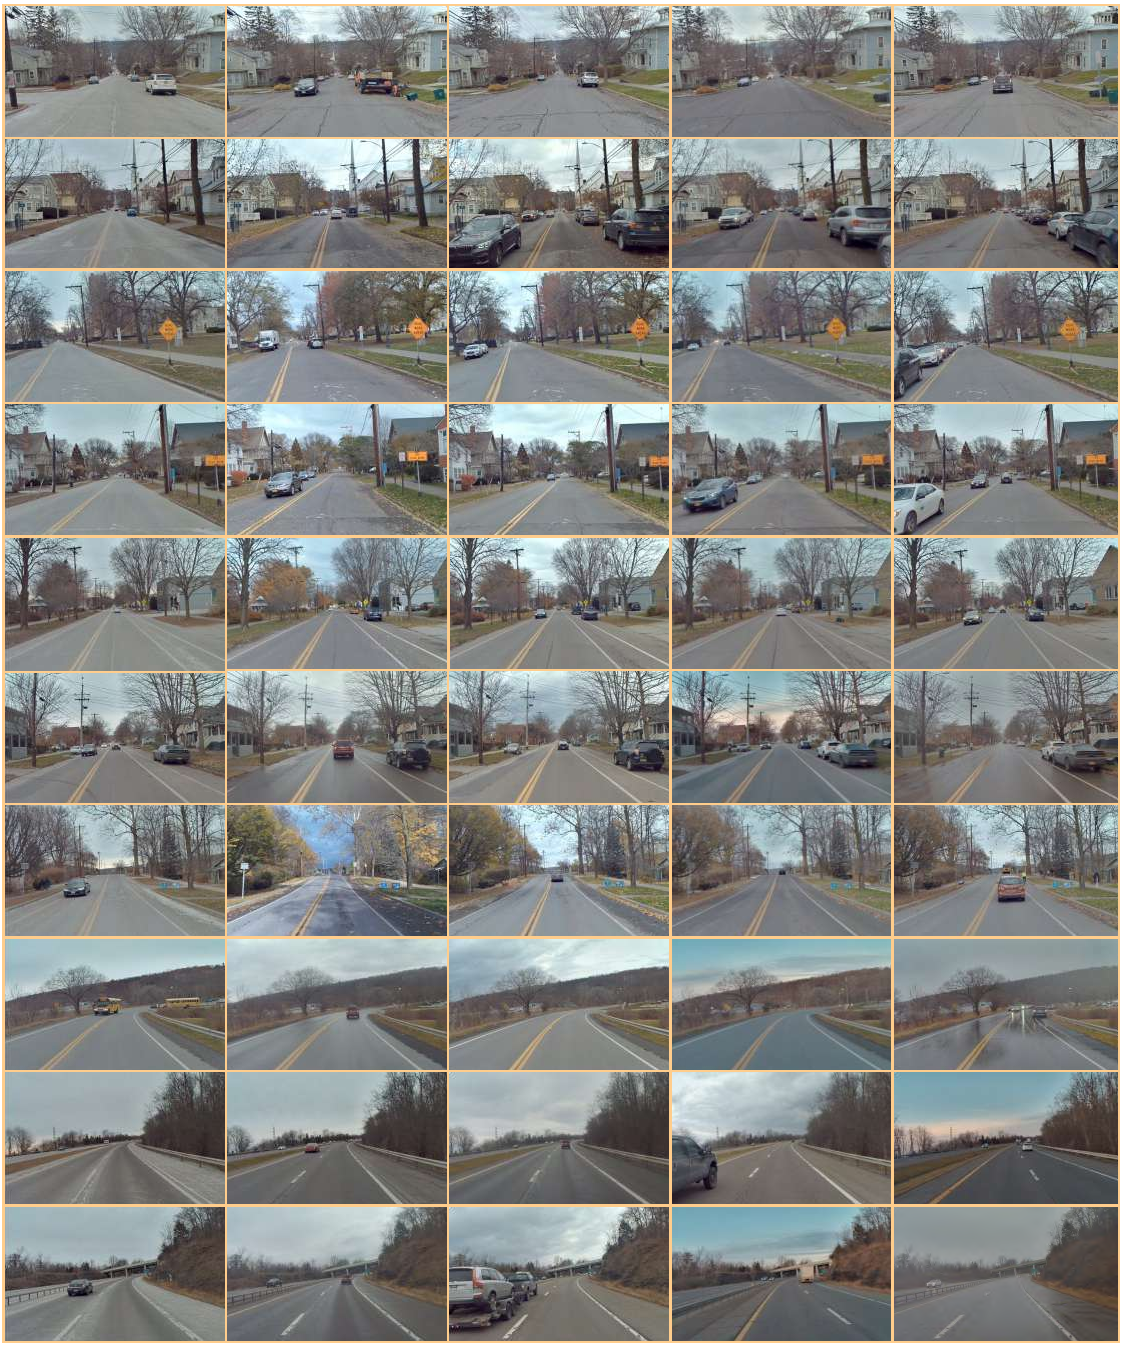
\includegraphics[width=0.95\linewidth]{figs_compressed/ithaca-1_compressed.pdf}
    \caption{\textbf{Visualizations of Mapverse-Ithaca365 dataset (locations 1-10).} Each row represents image observations of the same location captured during different traversals, with five traversals shown for brevity. The figure encompasses diverse environments in the Ithaca area, from residential neighborhoods with houses, trees, and varying traffic, to suburban streets with signage and seasonal foliage changes, and finally to rural roads and highways with expansive landscapes. The columns provide comparative views of these locations under different conditions, highlighting the dynamic nature of the Mapverse-Ithaca365 dataset.}
    \label{fig:ithaca-1}
\end{figure}

\begin{figure}
    \centering
    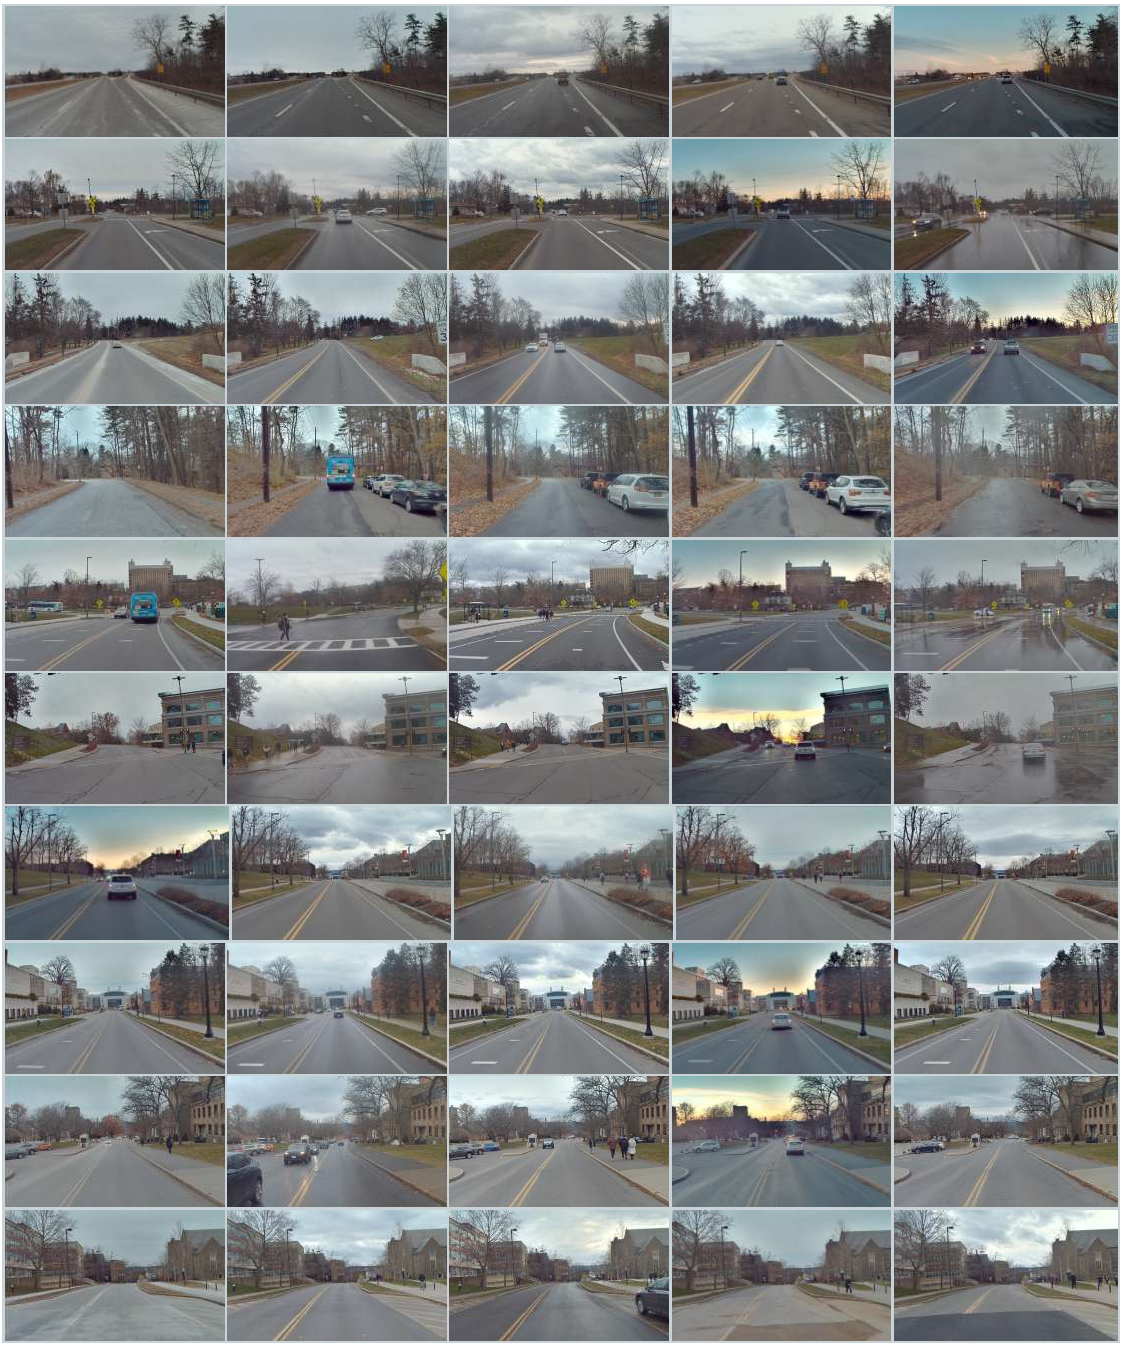
\includegraphics[width=1\linewidth]{figs_compressed/ithaca-2_compressed.pdf}
    \caption{\textbf{Visualizations of Mapverse-Ithaca365 dataset (locations 11-20).} Each row captures image observations of the same location from different traversals, showing five traversals for brevity. The figure spans various environments within Ithaca, from expansive rural highways transitioning to suburban roads with clear signage, to wooded areas with parked vehicles, and urban intersections with notable buildings. The images depict the progression from rural outskirts to more densely populated urban centers, reflecting changes in traffic, lighting, and seasonal foliage. Columns provide comparative views of these locations under different conditions, emphasizing the dynamic and diverse nature of the Mapverse-Ithaca365 dataset.}
    \label{fig:ithaca-2}
\end{figure}

\begin{figure}
    \centering
    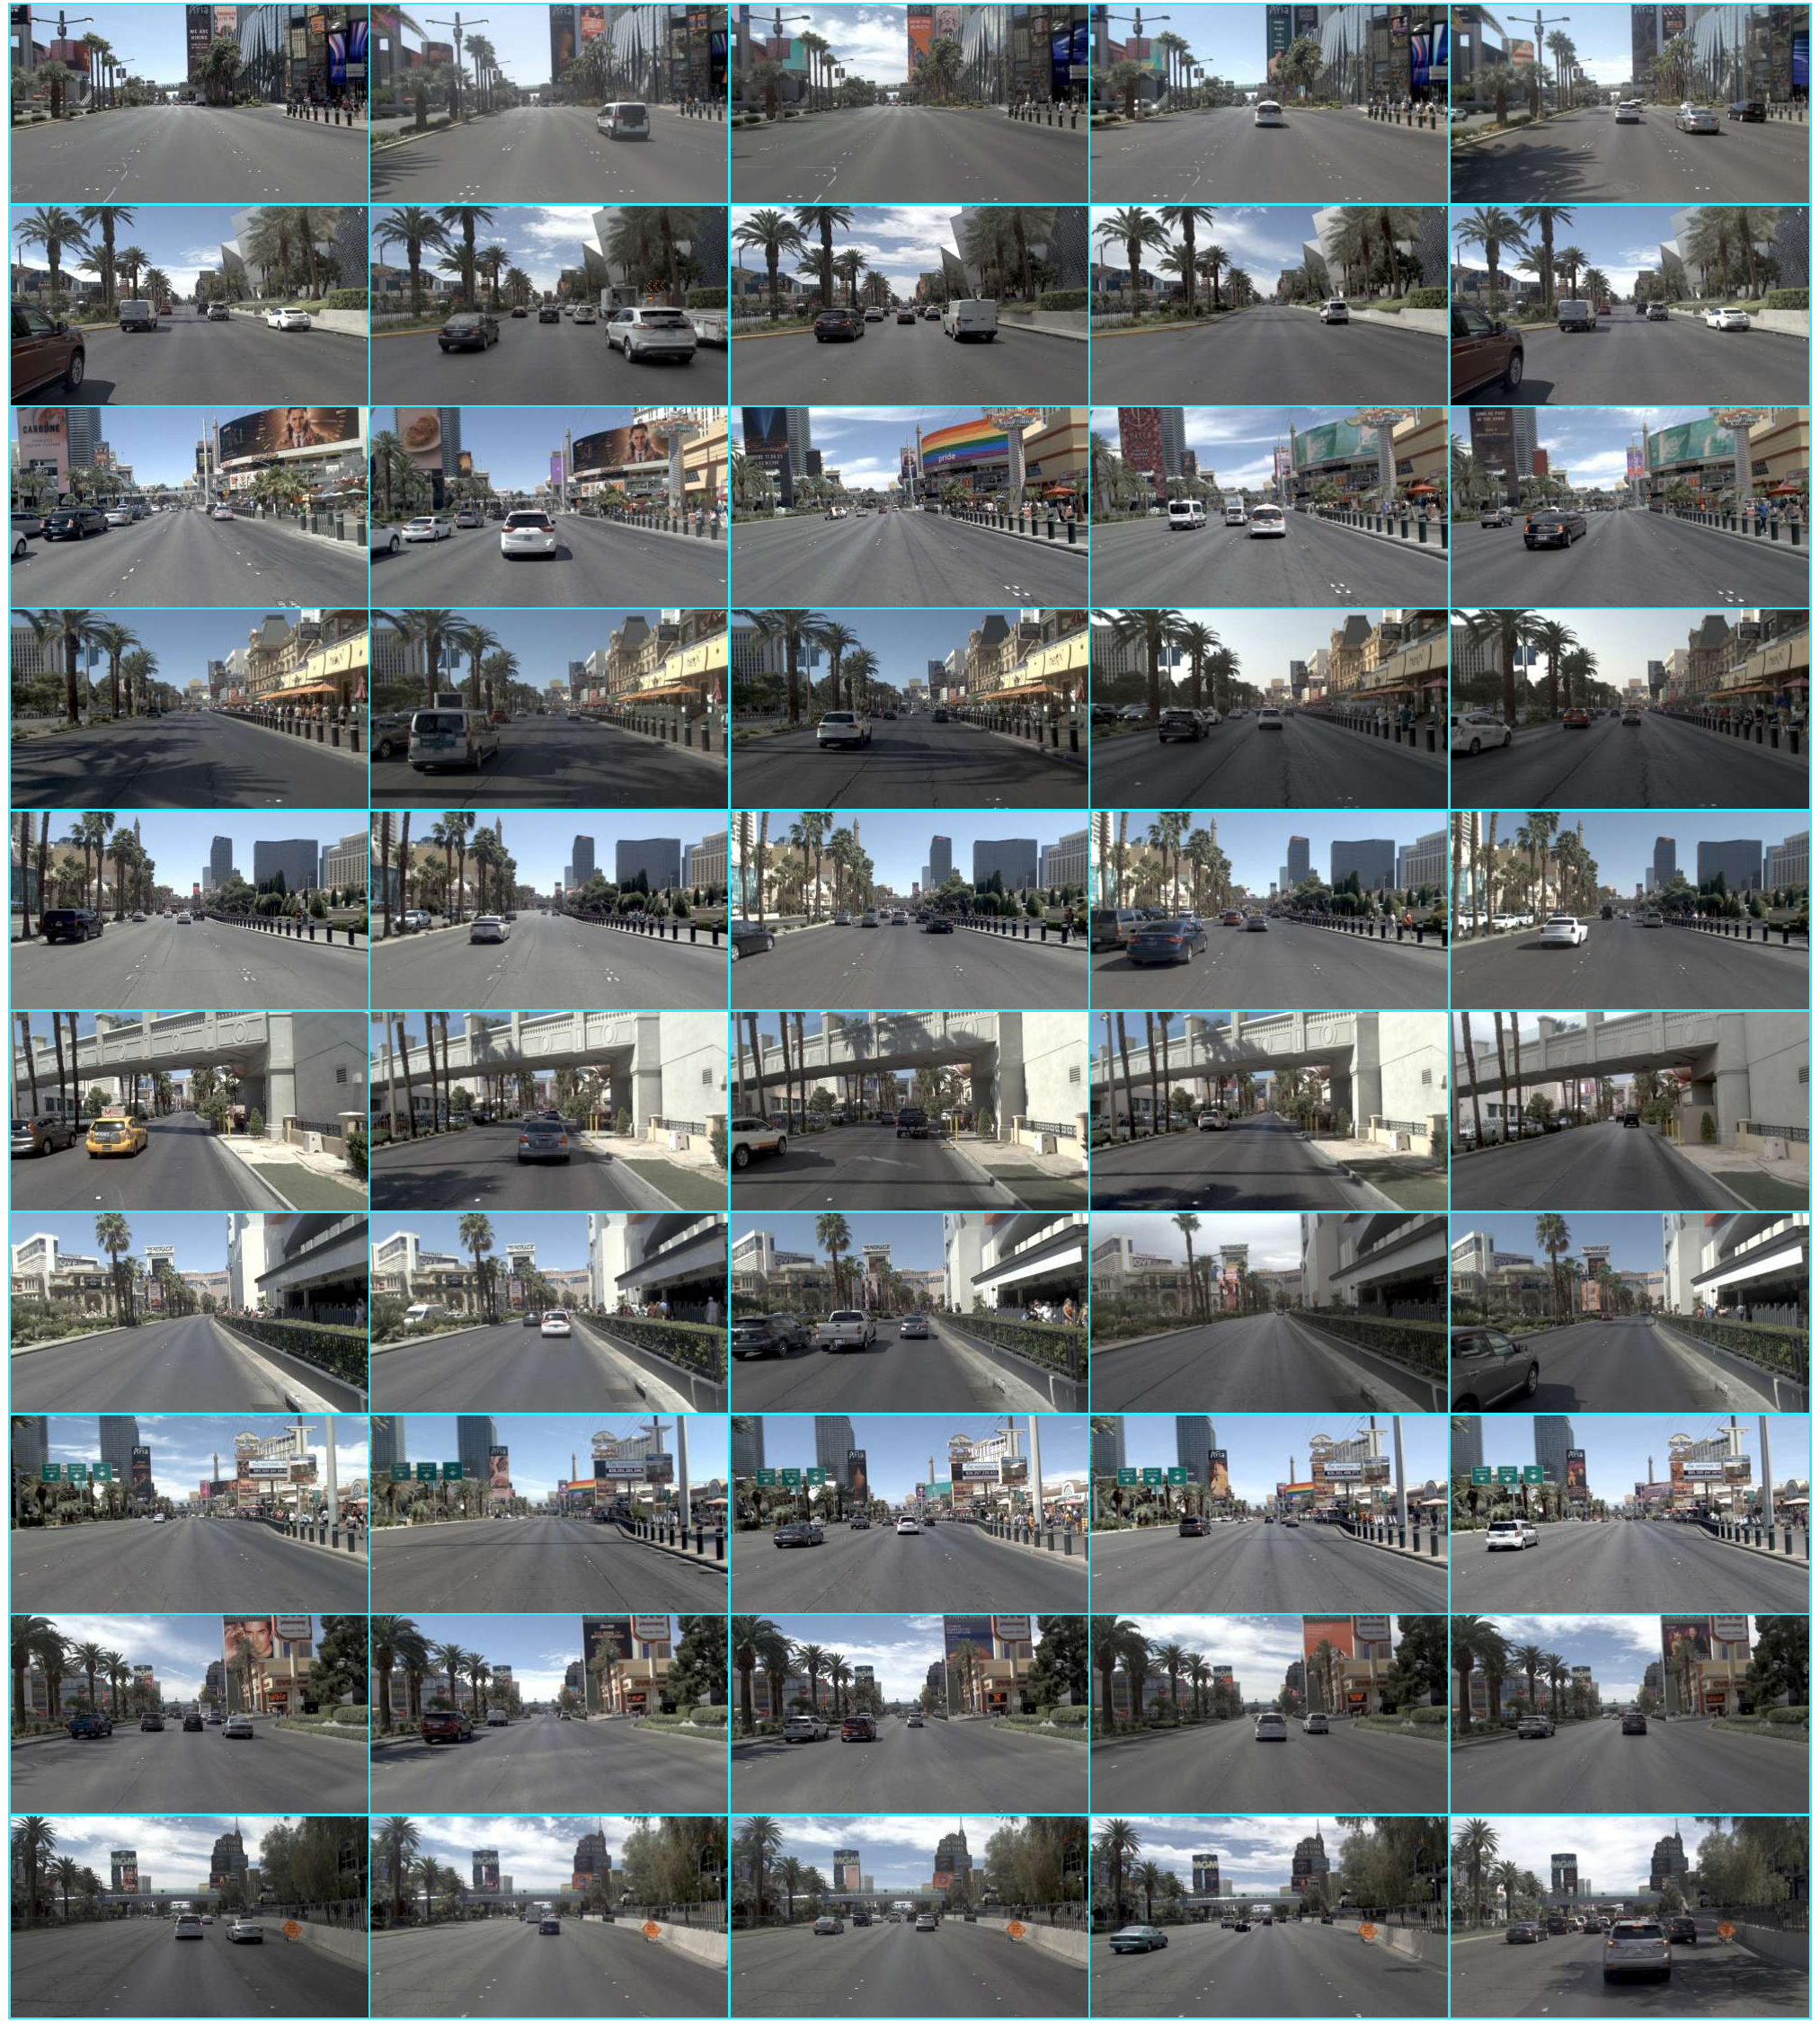
\includegraphics[width=1\linewidth]{figs_compressed/vegas-1_compressed.pdf}
    \caption{\textbf{Visualizations of Mapverse-nuPlan dataset (locations 1-10).} Each row represents different image observations of the same location captured during multiple traversals, with five shown for brevity. The images encompass diverse environments in Las Vegas, including wide city streets with iconic buildings, billboards, palm trees, pedestrian bridges, and varying traffic conditions.  Columns provide comparative views of the same locations under different conditions, illustrating the variability and complexity of the cityscape as captured in the Mapverse-nuPlan dataset.
}
    \label{fig:nuplan-1}
\end{figure}

\begin{figure}
    \centering
    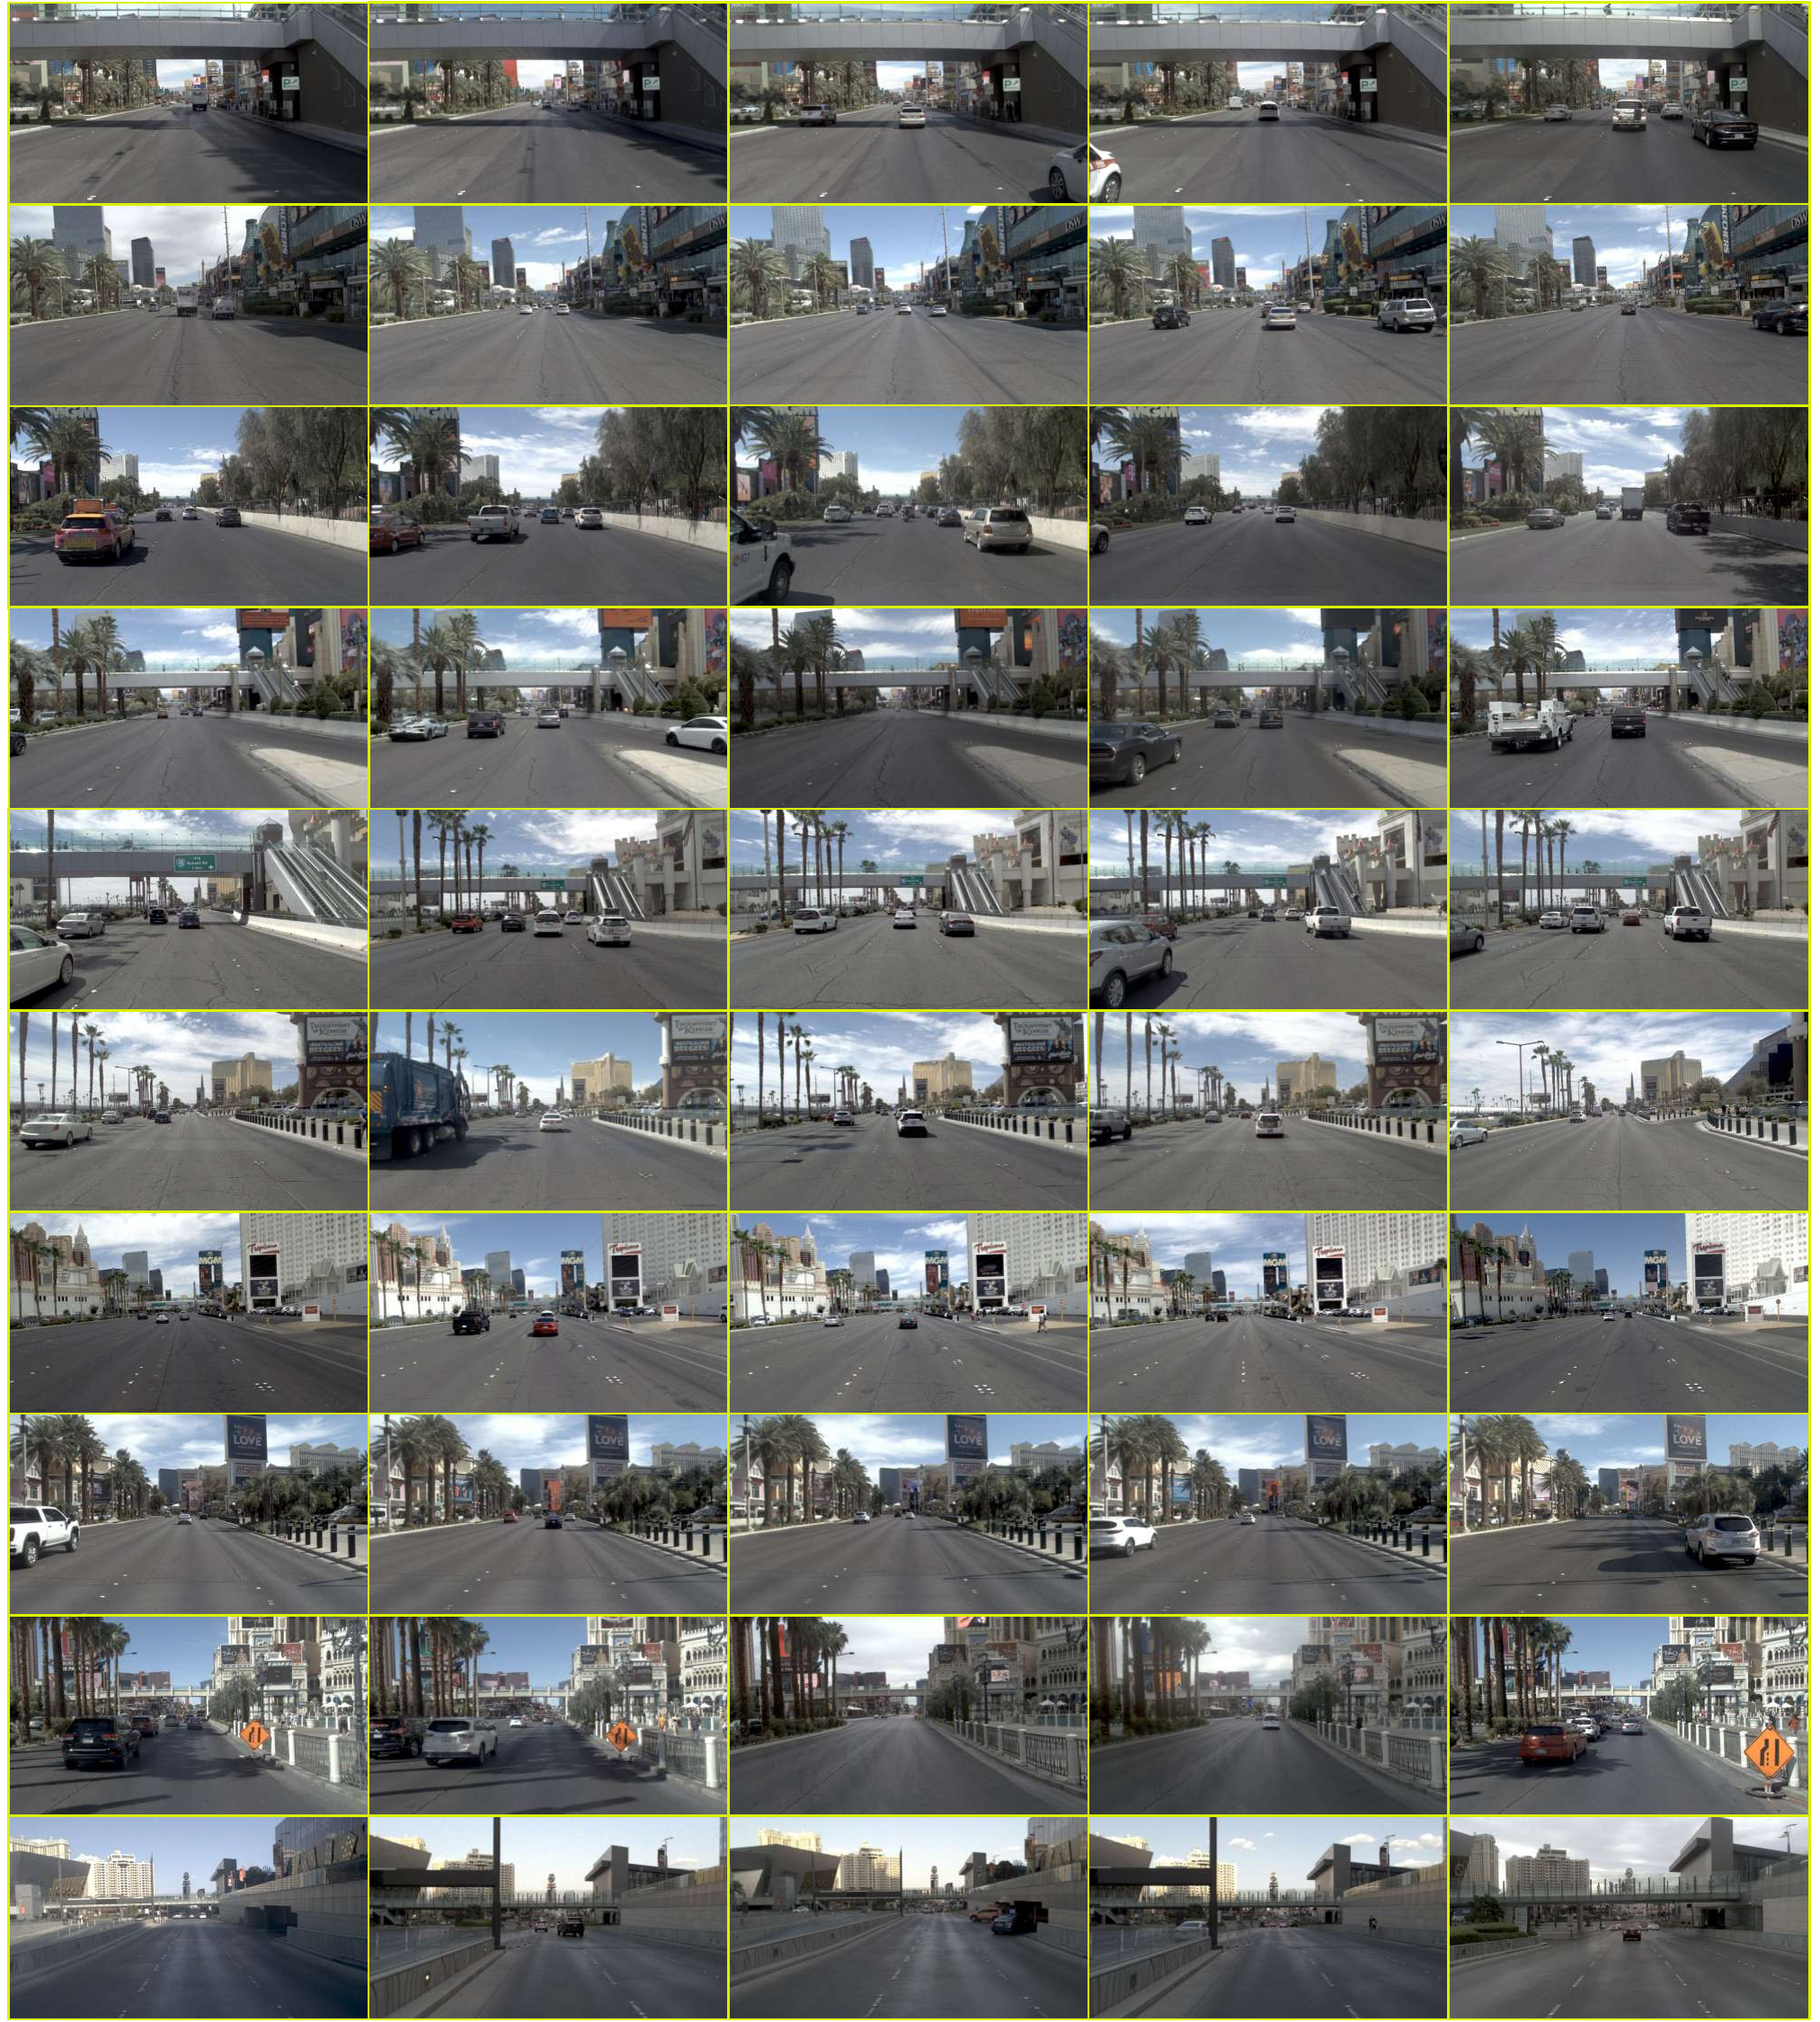
\includegraphics[width=1\linewidth]{figs_compressed/vegas-2_compressed.pdf}
    \caption{\textbf{Visualizations of Mapverse-nuPlan dataset (locations 11-20).} Each row represents different image observations of the same location captured during multiple traversals, with five shown for brevity. The images cover various environments in Las Vegas, including city streets with overpasses, iconic buildings, palm trees, billboards, and varied traffic conditions. The sequence progresses from urban settings with heavy infrastructure and prominent landmarks to broader streets and intersections, capturing different times of day and lighting conditions. Columns provide comparative views of the same locations under different circumstances, showcasing the dynamic and ever-changing urban landscape of Las Vegas as recorded in the Mapverse-nuPlan dataset.}
    \label{fig:nuplan-2}
\end{figure}


\clearpage


\section{Mapverse-Ithaca365: Additional Results of 2D Segmentation}
\subsection{Additional Qualitative Results}
\label{subsec:add-quali-appendix}
\begin{figure}[ht]
\begin{center}
\centerline{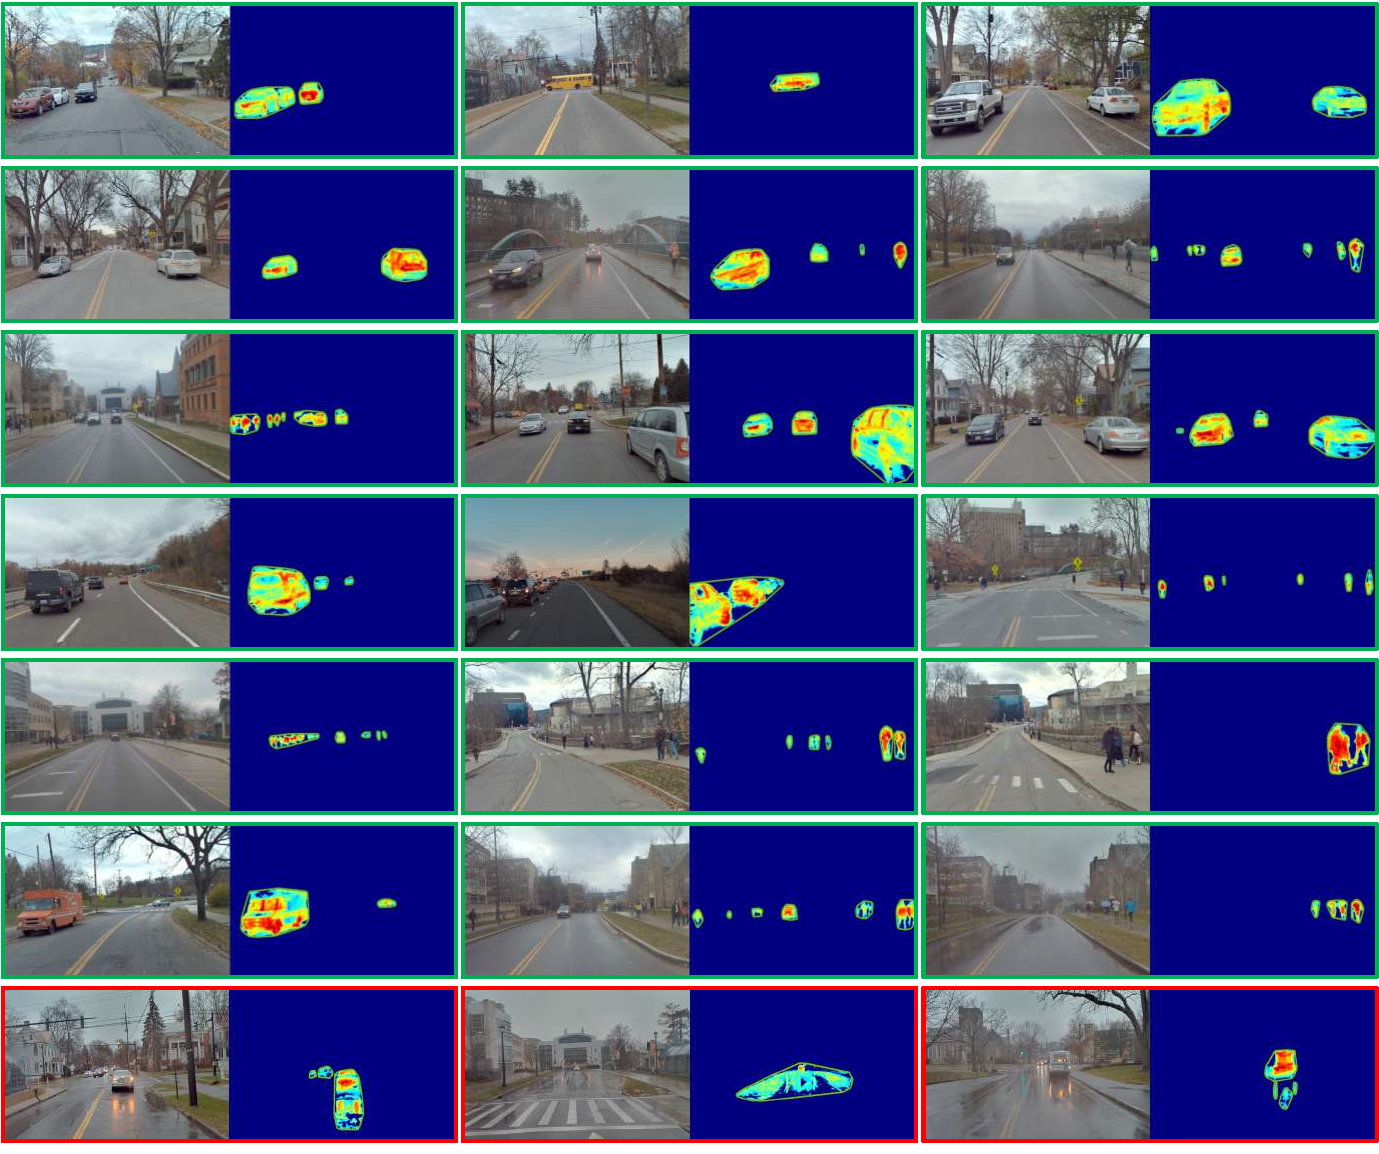
\includegraphics[width=\columnwidth]{figs_compressed/featmask-supp_compressed.pdf}}
\caption{\textbf{Qualitative evaluations of the emerged object masks}. Our method demonstrates robust performance across a range of lighting and weather conditions, effectively handling diverse categories including cars, buses, and pedestrians. Some failure cases are highlighted with red rectangles. }
\label{fig:visseg-appendix}
\end{center}
% \vspace{-10mm}
\end{figure}


\clearpage

\subsection{Visualizations of Supervised and Unsupervised Segmentation}


\label{subsec:vis-compareison-appendix}
\begin{figure}[ht]
\begin{center}
\centerline{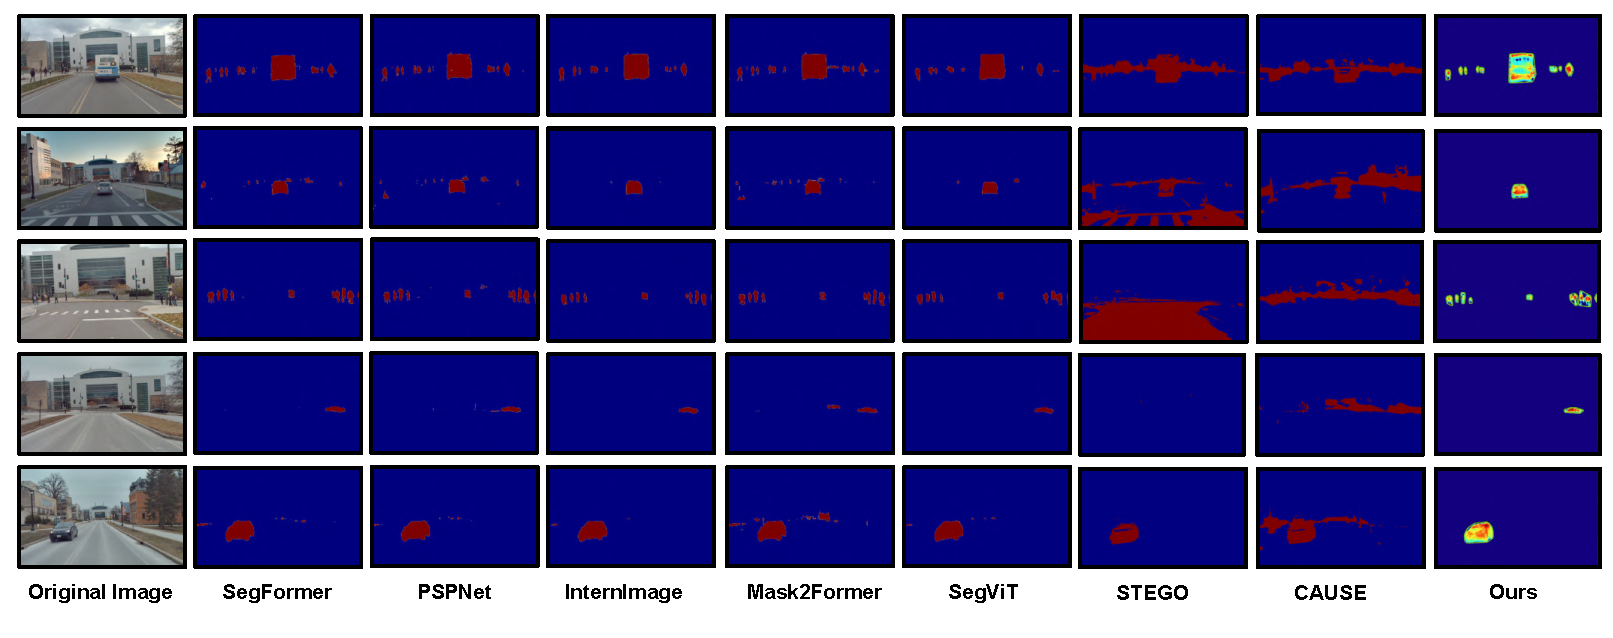
\includegraphics[width=\columnwidth]{figs_compressed/seg-compare_compressed.pdf}}
\caption{\textbf{Qualitative comparisons of our method and other supervised and unsupervised segmentation baselines.} This image demonstrates a comparison between our mask extraction and those derived from other semantic segmentation methods. The results indicate that our masks maintain superior integrity and detail in complex environments. Meanwhile, our method significantly outperforms unsupervised semantic segmentation models~\cite{hamilton2022unsupervised,kim2023causal} and is roughly equivalent to the masks generated by InternImage~\cite{wang2023internimage} and SegVit~\cite{zhang2022segvit}. Although Mask2Former~\cite{cheng2022masked}, PSPNet~\cite{zhao2017pspnet}, and SegFormer~\cite{xie2021segformer} have advantages in recognizing people and other fine-grained objects, they can also lead to incorrect segmentation and noise in certain scenarios. }
\label{fig:comparison-seg-appendix}
\end{center}
\vspace{-10mm}
\end{figure}

\clearpage

\subsection{Performance over Training Iterations }

Figure~\ref{fig:ablation-iteration-appendix} presents the IoU performance across iterations for two different feature resolutions (110×180 and 140×210), alongside visualizations of ephemerality masks and feature residuals at various iterations. The IoU graph on the left shows that both resolutions exhibit rapid improvement in the initial iterations, with the 110×180 resolution consistently outperforming the 140×210 resolution. The 110×180 resolution reaches an IoU of approximately 0.44, while the 140×210 resolution plateaus around 0.41. This indicates that the lower resolution (110×180) is more efficient in capturing ephemeral objects. On the right, the visualizations of ephemerality masks and feature residuals at different iterations (500 to 10000) demonstrate that higher iterations result in more detailed and accurate segmentation. Early iterations (500 and 1000) show sparse and less accurate masks. The progression also highlights the fast convergence of our method for effective segmentation.

\paragraph{Summary} In summary, the figure demonstrates that the 110×180 feature resolution is more effective and efficient for segmentation, achieving higher IoU scores compared to the 140×210 resolution. The IoU increases rapidly in the initial iterations and stabilizes around iteration 4000. These results emphasize the importance of selecting an appropriate feature resolution and ensuring sufficient iterations to achieve optimal segmentation performance.

\vspace{5mm}

\begin{figure}[ht]
\begin{center}
\centerline{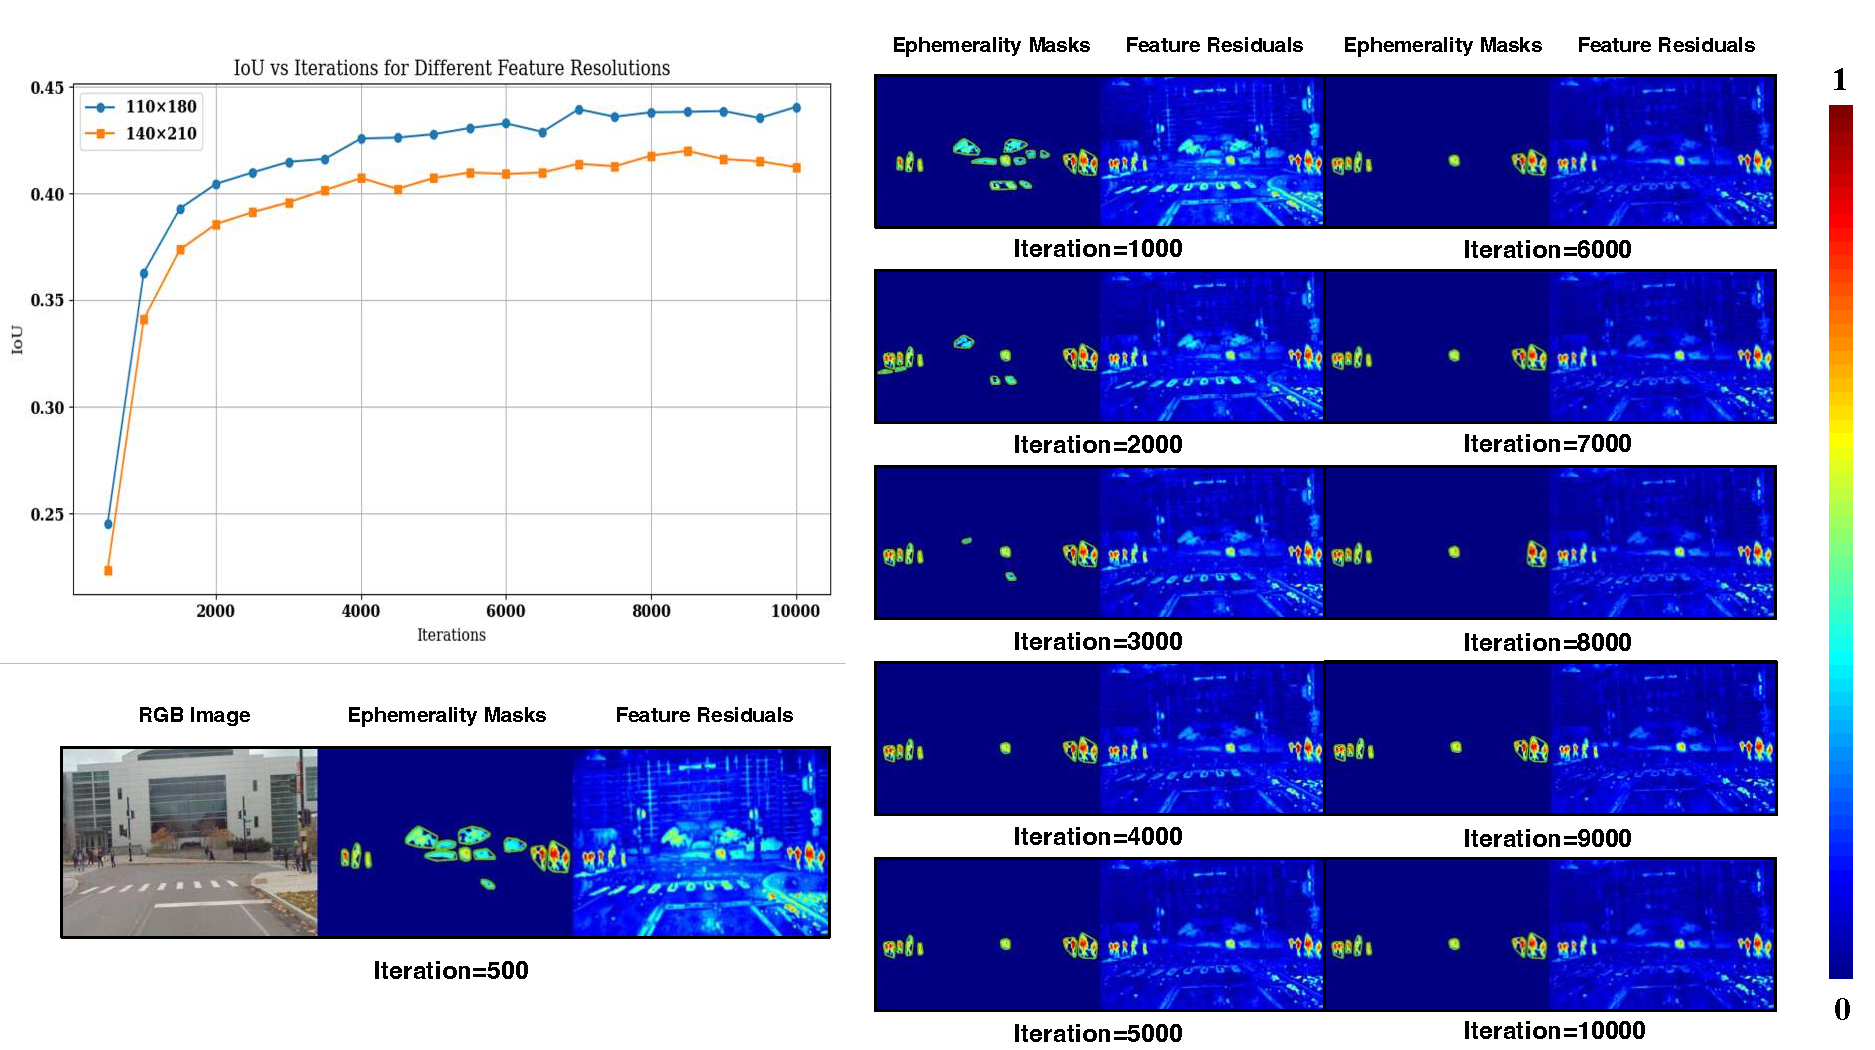
\includegraphics[width=\columnwidth]{figs_compressed/ablation-iteration_compressed.pdf}}
\caption{ \textbf{IoU performance over iterations for different feature resolutions (110×180 and 140×210) and corresponding visualizations of ephemerality masks and feature residuals.} Visualizations at various iterations (500 to 10000) illustrate that higher iterations lead to more detailed and accurate segmentation. The results highlight the efficiency of the 110×180 resolution and the fast convergence of our method for effective segmentation.}
\label{fig:ablation-iteration-appendix}
\end{center}
\end{figure}





\clearpage




\subsection{Ablation Study on Number of Traversal: Visualization and Discussion}

Figure~\ref{fig:ablation-traversal-appendix} showcases the segmentation performance of \texttt{EmerSeg} with images collected from varying numbers of traversals. Each row represents a different scene, while the columns illustrate the results from 1, 2, 3, 7, and 10 traversals, respectively. The segmentation map with a single traversal shows minimal detection of ephemeral objects, indicating limited information for effective segmentation. For example, the method fails to segment three parked buses in the first row due to a lack of diverse visual observations, which are crucial for our model to localize these transient yet static objects. With 2 traversals, there is a significant improvement in segmentation performance. The segmentation map reveals larger and more distinct objects, demonstrating the benefit of additional traversals. Segmentation performance with 10 traversals is similar to that with 7 traversals. Objects are detected reliably, but the improvement beyond 7 traversals is marginal, indicating diminishing returns.


\paragraph{Summary} Figure~\ref{fig:ablation-traversal-appendix} illustrates the clear trend of improving segmentation performance with an increasing number of traversals. The results indicate that while significant gains are achieved with additional traversals, the benefits plateau after a certain point. This analysis underscores the importance of multiple traversals for effective segmentation while suggesting an optimal balance between the number of traversals and segmentation accuracy.


\vspace{5mm}


\begin{figure}[ht]
\begin{center}
\centerline{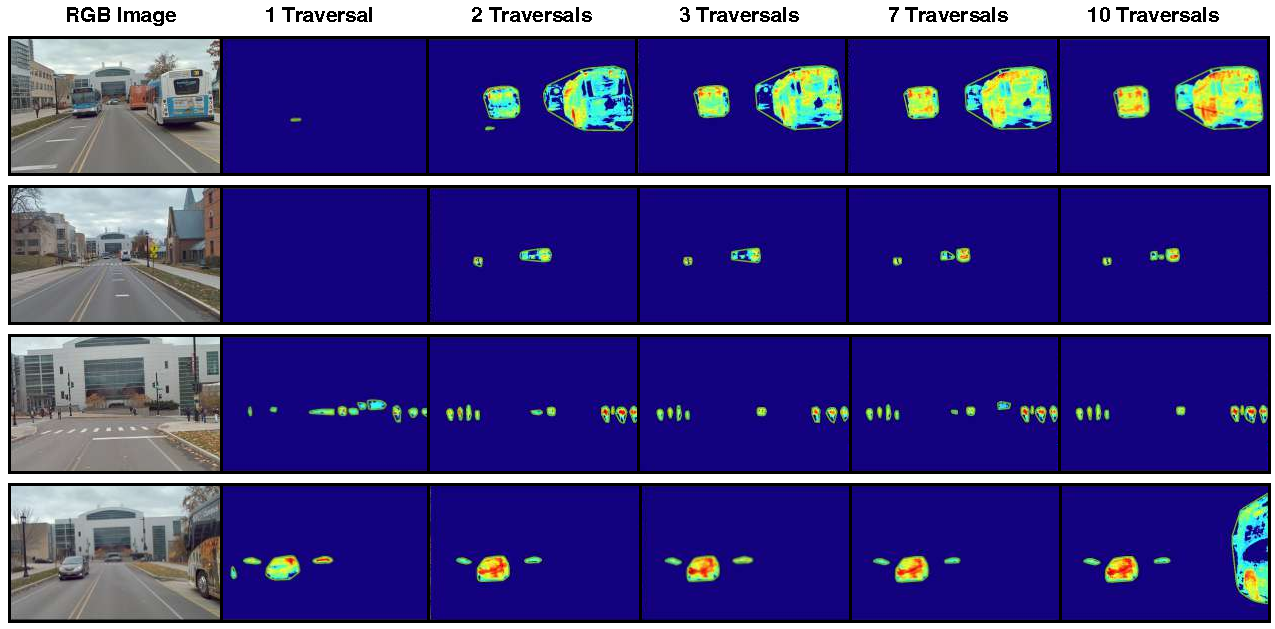
\includegraphics[width=\columnwidth]{figs_compressed/ablation-traversal_compressed.pdf}}
\caption{\textbf{Visualizations of \texttt{EmerSeg} with inputs from different numbers of traversals.} Each row represents a different scene of a location. The first column shows the original RGB images. The subsequent columns show the segmentation outputs from \texttt{EmerSeg} with 1, 2, 3, 7, and 10 traversals.}
\label{fig:ablation-traversal-appendix}
\end{center}
\end{figure}

\clearpage





\subsection{Ablation Study on Feature Dimension: Visualization and Discussion}

Figure~\ref{fig:ablation-dimension-appendix} illustrates the impact of varying feature dimensions on the segmentation performance. At the lowest dimension (4), the ephemerality masks are sparse, capturing very few objects with minimal detail since the feature residuals are not discriminative, indicating insufficient feature representation. A substantial enhancement is observed at dimension 16, where the ephemerality masks become more detailed, capturing more objects with better clarity. At the highest dimension (64), the segmentation is highly detailed and accurate, with ephemerality masks capturing a wide range of objects and feature residuals being informative, suggesting a comprehensive feature representation.

\paragraph{Summary} In summary, the segmentation performance improves significantly with increased feature dimensions. Low-dimensional features (4 and 8) fail to provide adequate information for accurate segmentation, resulting in sparse segmentation. A higher dimension (16 and 64) offers a substantial improvement, capturing most objects with clearer details. This demonstrates that higher-dimensional features are crucial for achieving accurate and comprehensive segmentation performance.

\vspace{5mm}

\begin{figure}[ht]
\begin{center}
\centerline{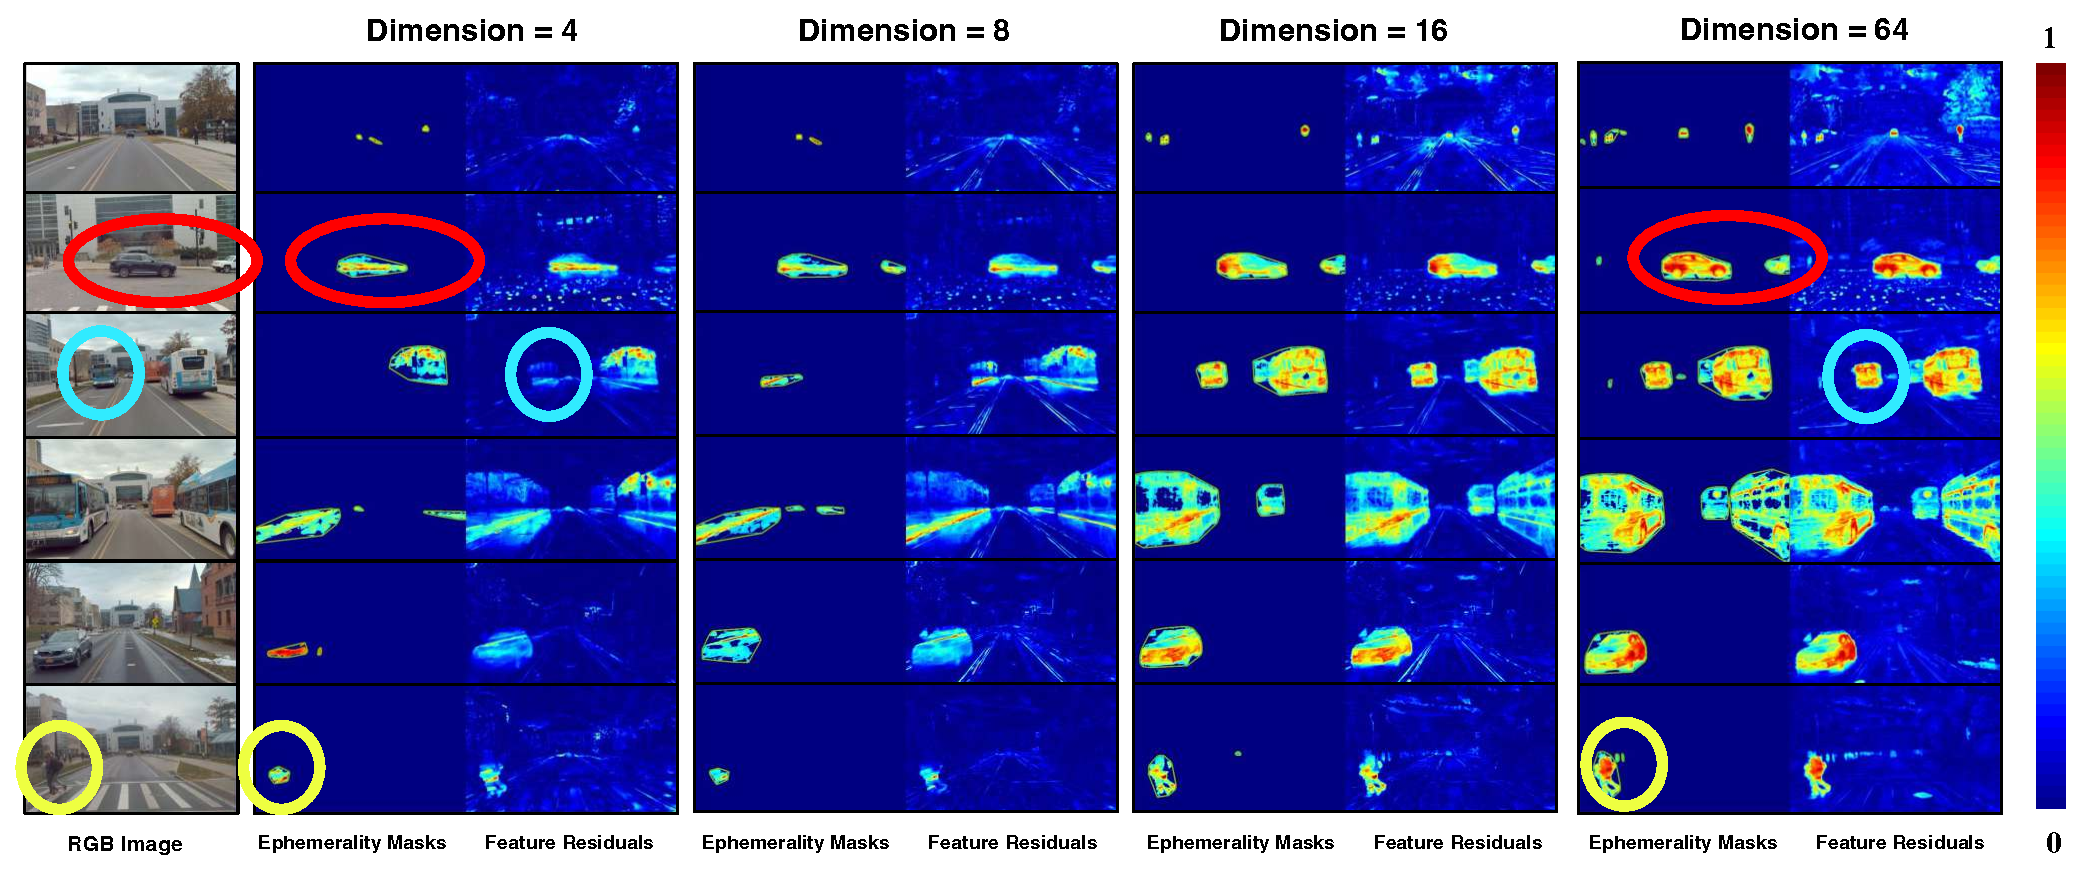
\includegraphics[width=\columnwidth]{figs_compressed/ablation-dimension_compressed.pdf}}
\caption{\textbf{Visualizations of ephemerality masks and feature residuals at different feature dimensions.} The RGB images (leftmost column) are processed to generate ephemerality masks and feature residuals. As the feature dimensions increase, the segmentation accuracy improves, with the highest dimension (64) capturing the most detailed and accurate object masks. The residuals are more discriminative with higher dimensions, indicating better feature representation. The colored circles highlight specific areas to illustrate differences in segmentation quality across dimensions.}
\label{fig:ablation-dimension-appendix}
\end{center}
\end{figure}

\clearpage




\subsection{Ablation Study on Feature Resolution: Visualization and Discussion}

Figure~\ref{fig:ablation-resolution-appendix} presents the segmentation performance at different feature resolutions: 25×40, 50×80, 70×110, and 110×180. The RGB images on the left are segmented into ephemerality masks and feature residuals for each resolution. At the lowest resolution (25×40), the ephemerality masks capture very few objects with minimal detail. As the resolution increases, there is a noticeable improvement in object segmentation, with more objects being identified. 

\paragraph{Summary} In a word, the segmentation performance improves significantly with increased feature resolution. Lower resolutions (25×40 and 50×80) result in sparse object segmentation, indicating inadequate feature representation. The highest resolution (110×180) delivers the best results, with detailed and precise segmentation. 

\vspace{5mm}
\begin{figure}[ht]
\begin{center}
\centerline{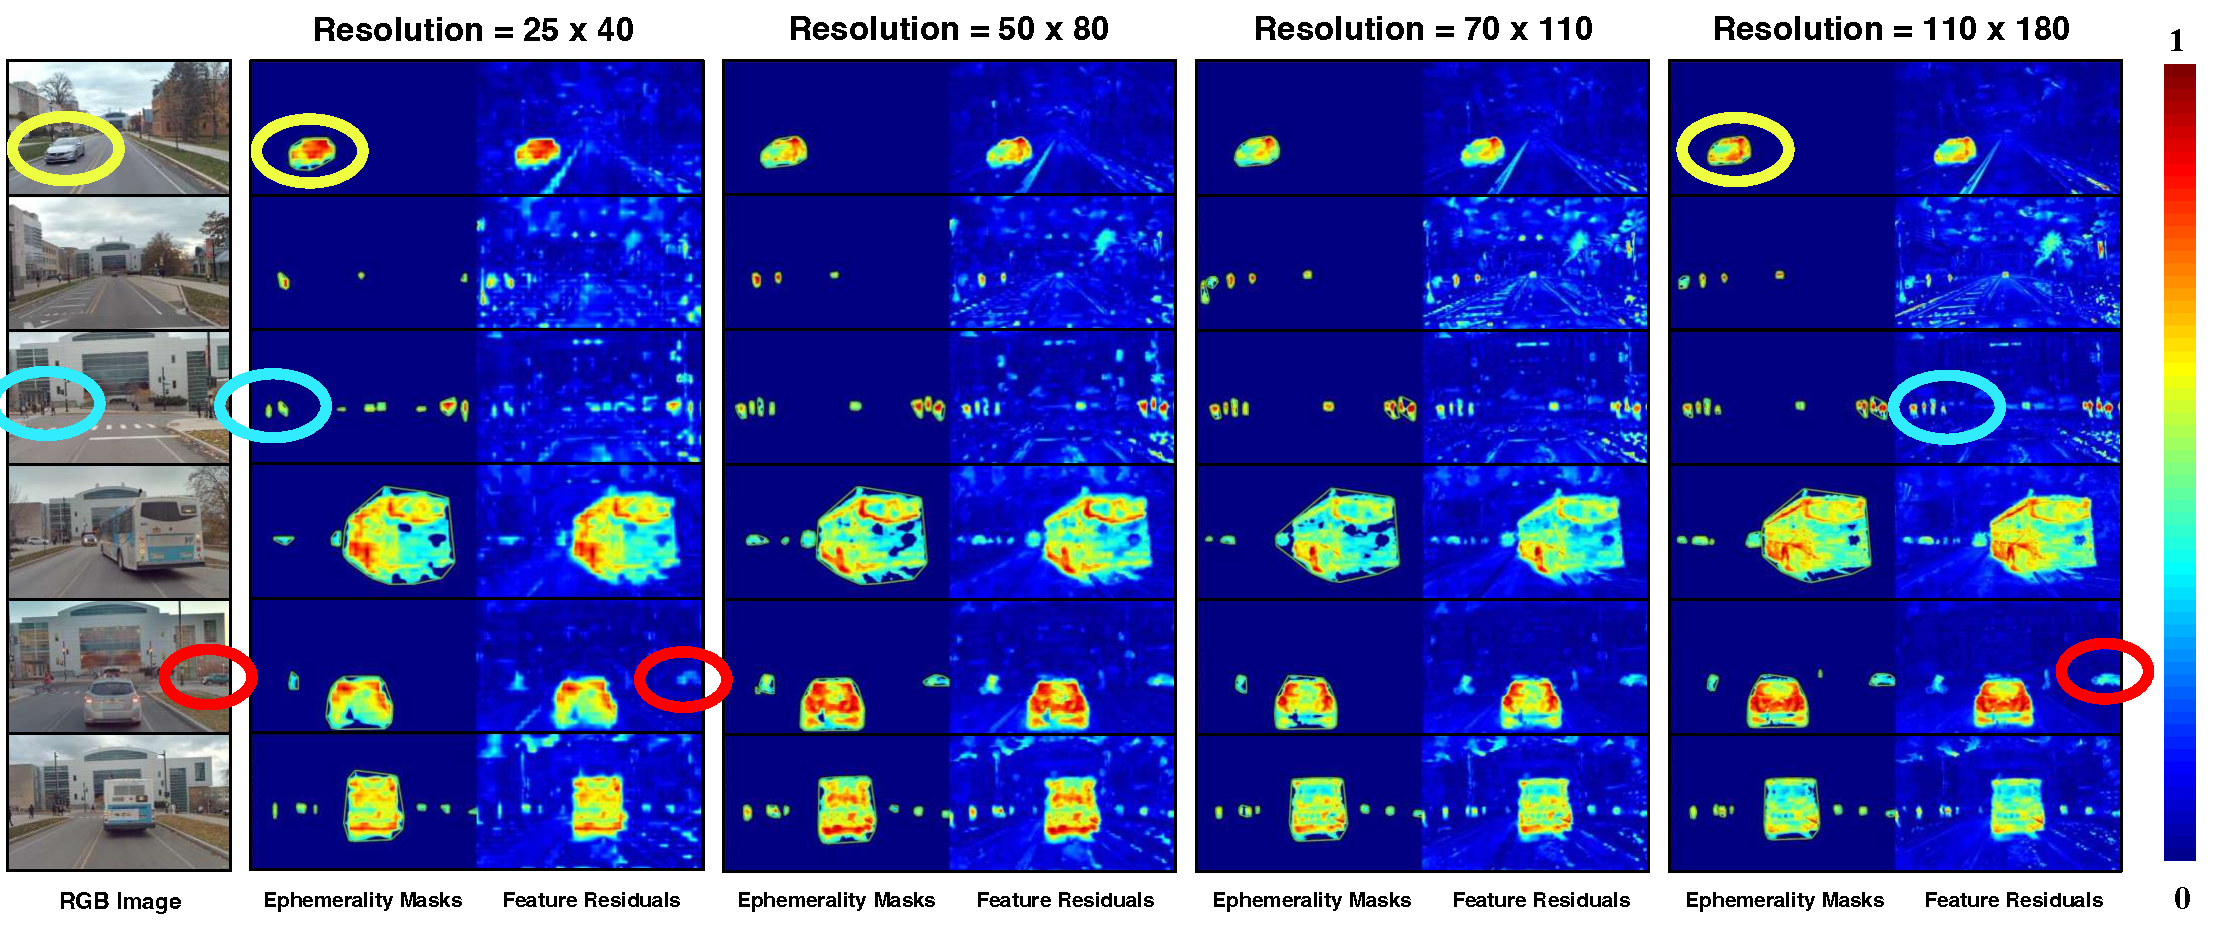
\includegraphics[width=\columnwidth]{figs_compressed/ablation-resolution_compressed.pdf}}
\caption{\textbf{Visualizations of ephemerality masks and feature residuals at different feature (spatial) resolutions.} The RGB images (leftmost column) are processed to generate ephemerality masks and feature residuals. As the feature resolution increases, the segmentation accuracy improves, with the highest resolution (110×180) capturing the most detailed and accurate object masks. The residuals are more informative with higher resolutions, indicating better feature representation and reduced segmentation errors. The colored circles highlight specific areas to illustrate differences in segmentation quality across resolutions.}
\label{fig:ablation-resolution-appendix}
\end{center}
\end{figure}



\clearpage






\subsection{Ablation Study on Vision Foundation Model: Visualization and Discussion}

Figure~\ref{fig:ablation-backbone-appendix} compares the performance of different versions and configurations of the DINO model on ephemerality masks and feature residuals. For both DINOv1 and DINOv2, the raw versions show noisy feature residuals, indicating areas where the model fails to capture ephemeral objects accurately. The denoised versions show a notable improvement, with informative residuals and more accurate ephemerality masks. The DINOv2 models generally perform better than DINOv1, as evidenced by more precise object masks and more discriminative residuals. The inclusion of the register in DINOv2 does not introduce additional gains.

\paragraph{Summary} The result highlights the progressive improvements in segmentation accuracy achieved through model evolution from DINOv1 to DINOv2, and the benefits of applying denoising techniques. 

\vspace{5mm}
\begin{figure}[ht]
\begin{center}
\centerline{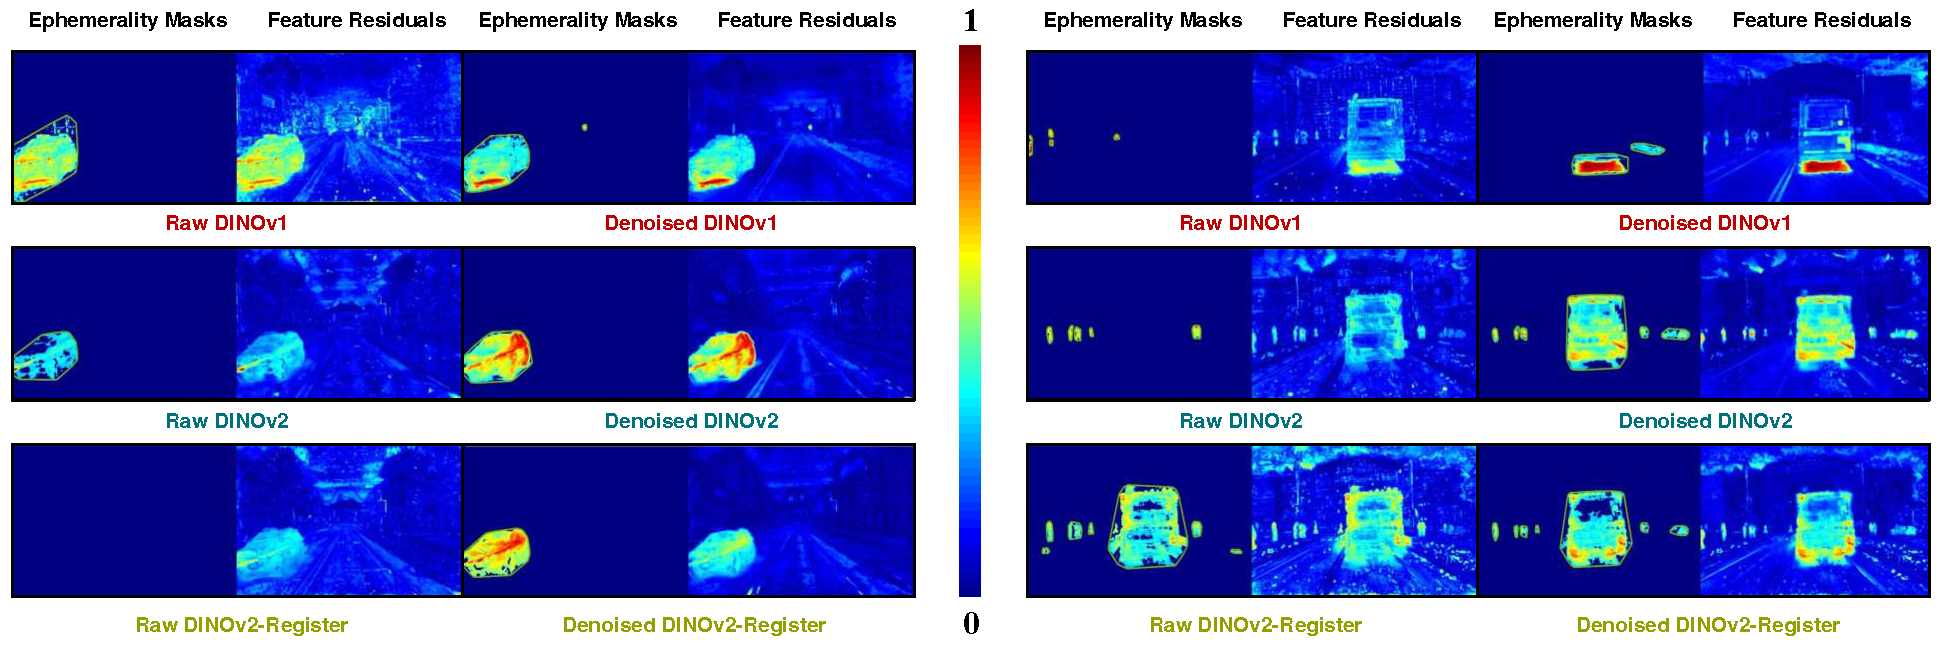
\includegraphics[width=\columnwidth]{figs_compressed/ablation-backbone_compressed.pdf}}
\caption{\textbf{Comparison of ephemerality masks and feature residuals using different versions of the DINO model.} The figure includes raw and denoised versions of DINOv1 and DINOv2, as well as raw and denoised versions of DINOv2 with a registration module (DINOv2-Register). Denoising enhances the quality of feature residuals, while registration does not yield notable gains.}
\label{fig:ablation-backbone-appendix}
\end{center}
\end{figure}



\clearpage



\section{Mapverse-Ithaca365: Additional Visualizations of 3D Reconstruction}
Figure~\ref{fig:reconstruction-appendix} compares Structure from Motion (SfM) initialized points with Gaussian points after optimization. On the left, the images display the raw data points obtained from the SfM process, which serves as an initial guess for the 3D structure of the environment. These points tend to be more scattered and less organized. On the right, the images show the Gaussian points after optimization, where the point cloud data has been refined through differentiable rendering. This refinement results in a more coherent and precise representation of the scene, as evidenced by the clearer and more defined structures in the point clouds. The comparison across various scenes highlights the effectiveness of the optimization process in enhancing the accuracy and clarity of the 3D reconstructed environment, crucial for applications in autonomous driving and robotics. 

\begin{figure}[ht]
    \centering
    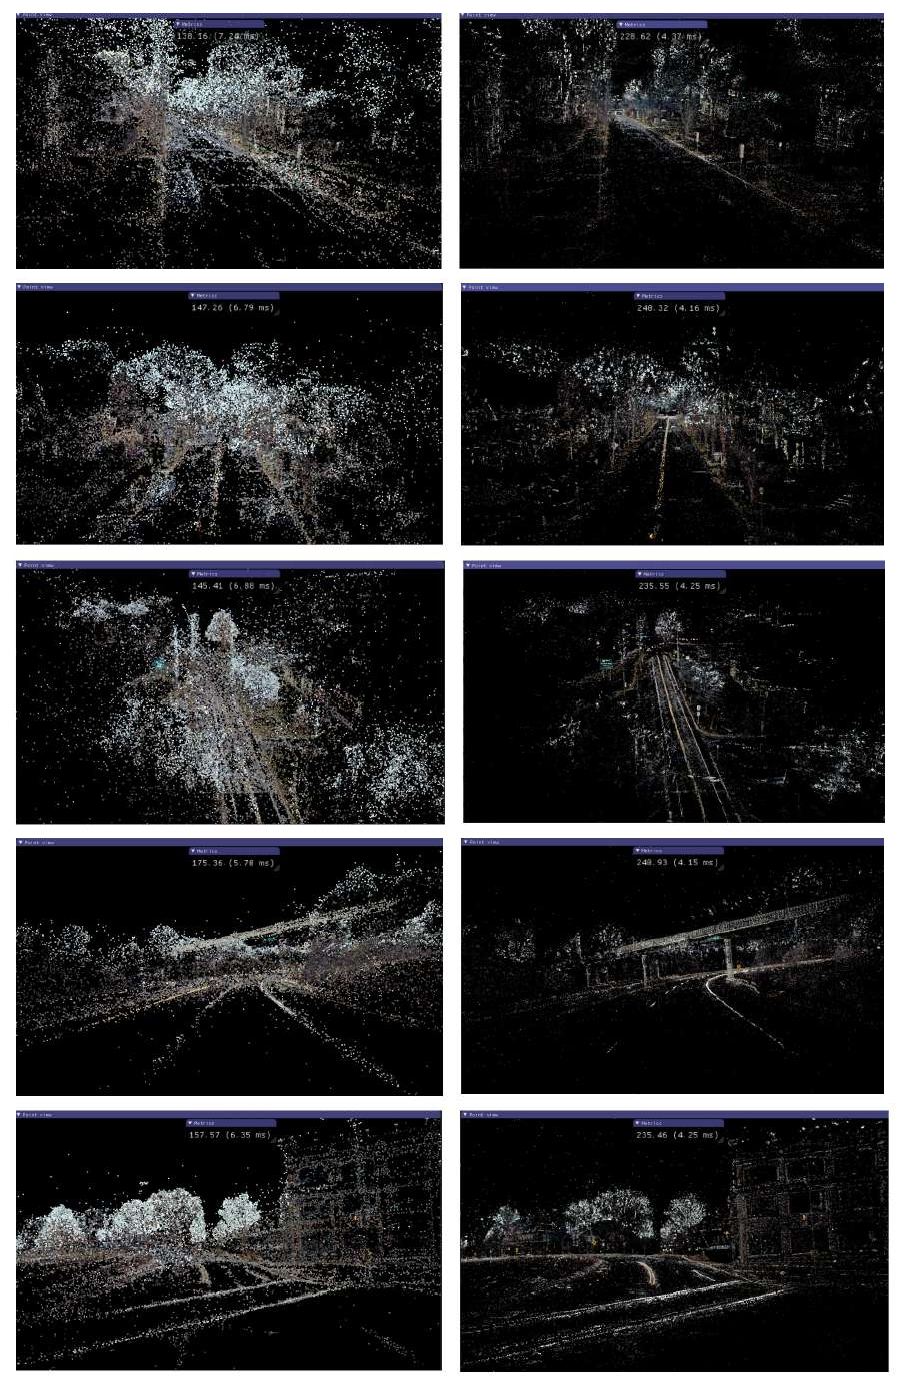
\includegraphics[width=0.8\linewidth]{figs_compressed/reconstruction_compressed.pdf}
    \caption{\textbf{Left: SfM Initialized Points. Right: Gaussian Points after Optimization.}}
    \label{fig:reconstruction-appendix}
\end{figure}


\begin{figure}[ht]
    \centering
    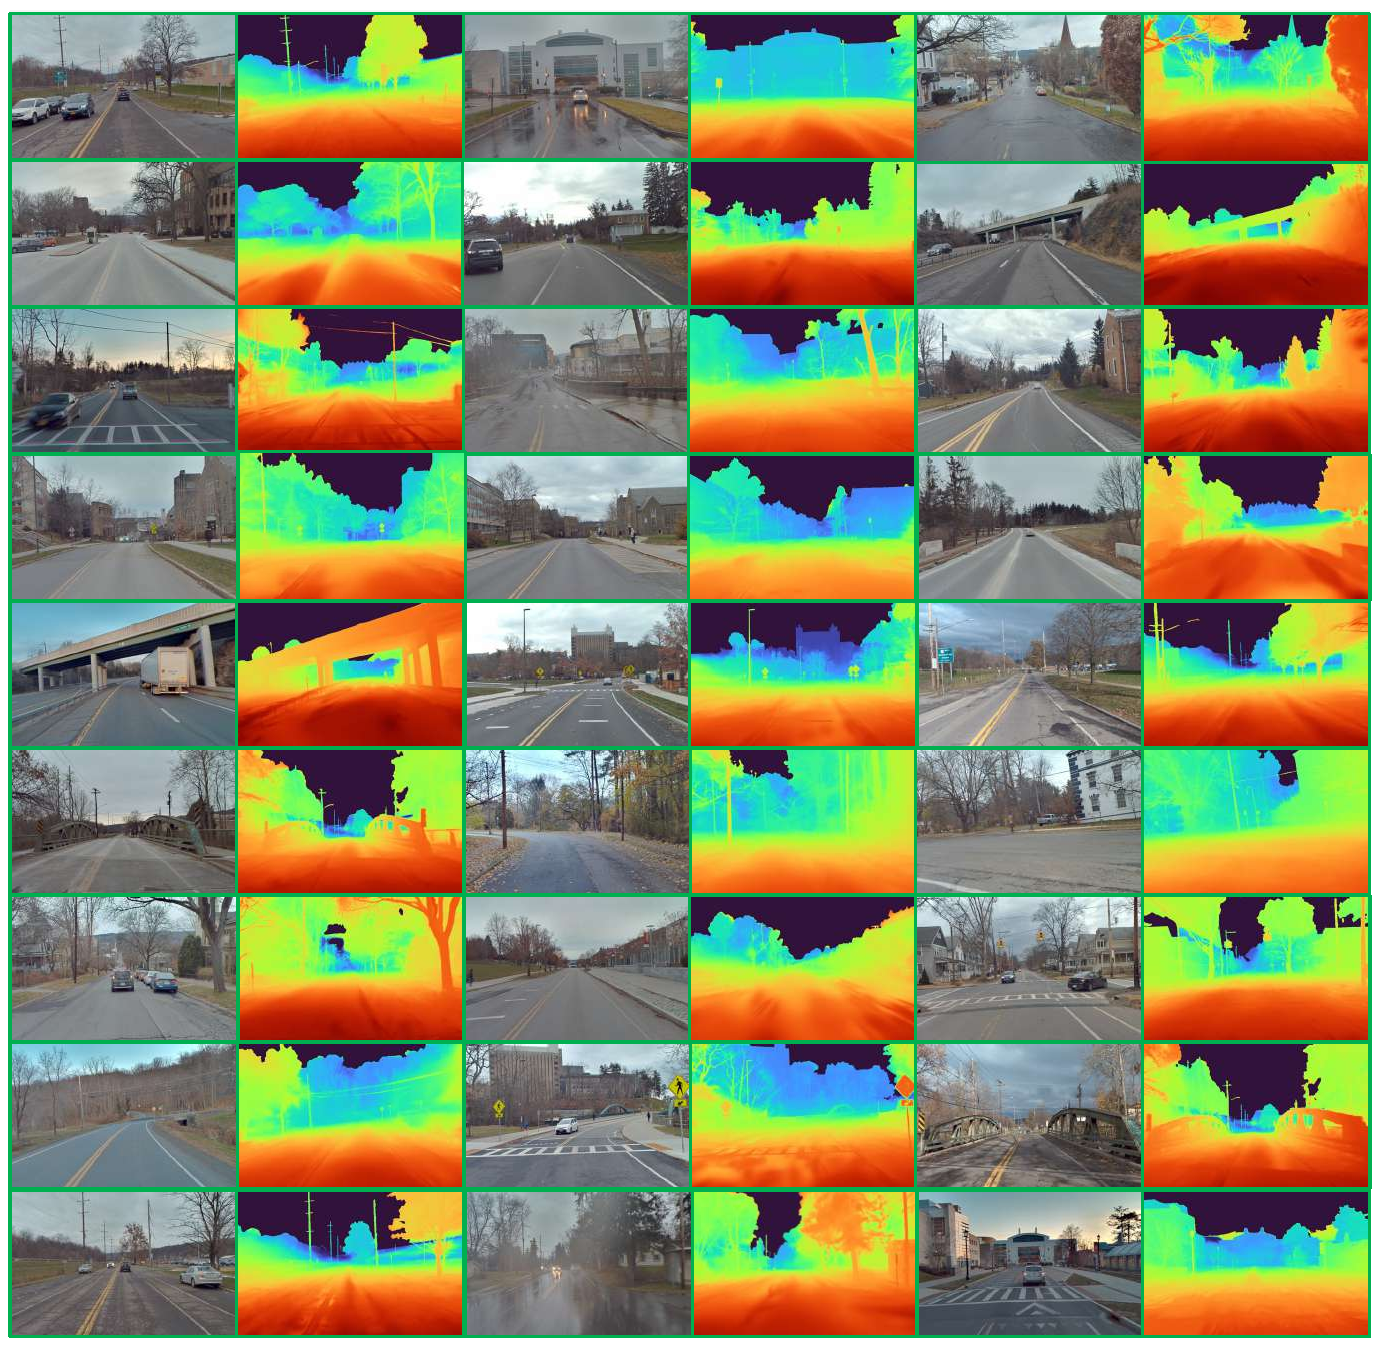
\includegraphics[width=\linewidth]{figs_compressed/ithaca-depth-app_compressed.pdf}
    \caption{\textbf{Visualizations of depth images in Mapverse-Ithaca365}}
    \label{fig:ithaca-depth-appendix}
\end{figure}


\clearpage


\section{Mapverse-Ithaca365: Additional Visualizations of Neural Rendering}

\begin{figure}[ht]
\begin{center}
\centerline{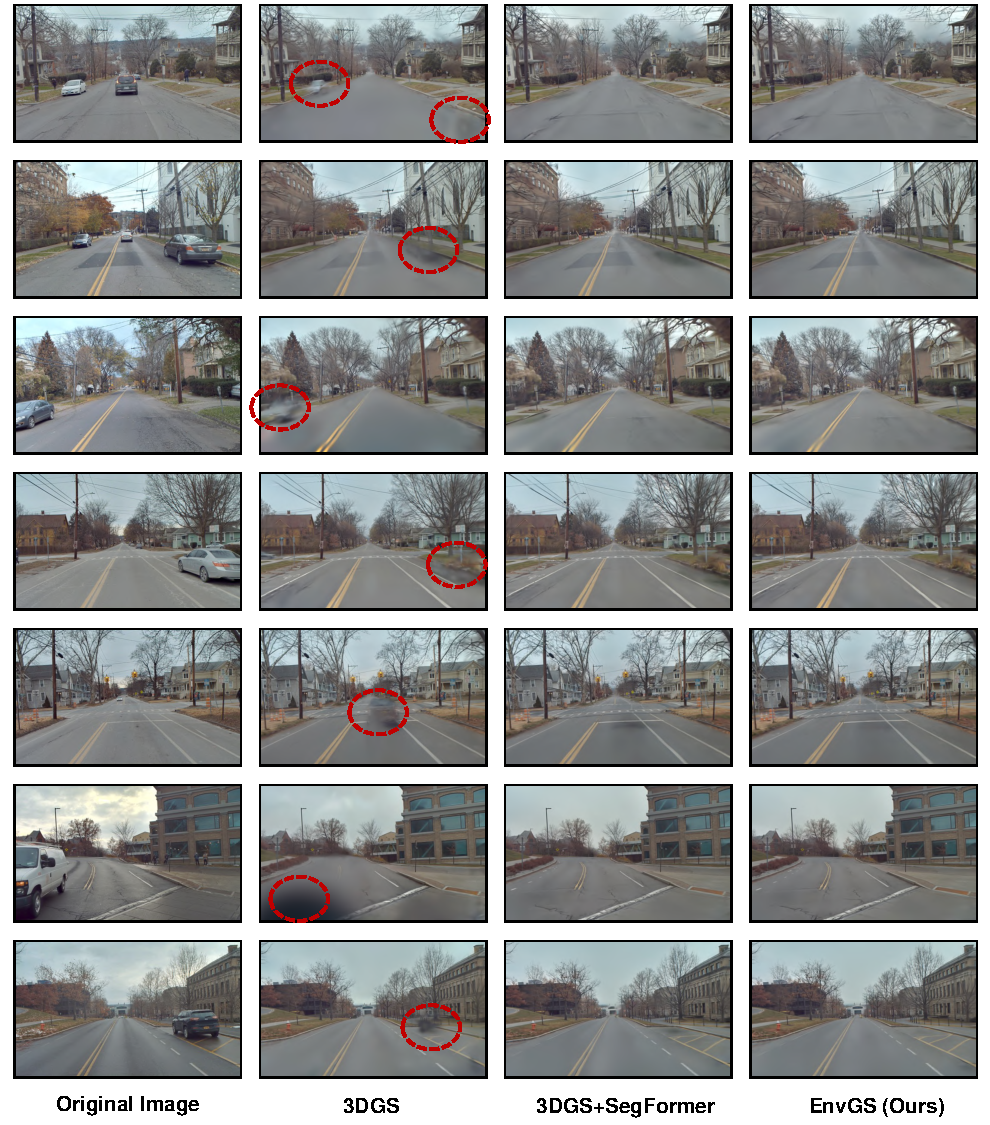
\includegraphics[width=\columnwidth]{figs_compressed/envrendering-supp_compressed.pdf}}
\caption{\textbf{Qualitative evaluations of the environment rendering.} Our method demonstrates robust performance against transient objects.}
\label{fig:rendering-appendix}
\end{center}
\vspace{-10mm}
\end{figure}


\clearpage


\section{Mapverse-nuPlan: Unsupervised 2D Segmentation}
\label{sec:seg-nuplan-app}
\subsection{Quantitative Results}

We employ SegFormer~\cite{xie2021segformer} to generate pseudo ground-truth masks and compare these with the output of \texttt{EmerSeg} using Intersection over Union (IoU) metrics in Mapverse-nuPlan collected in Las Vegas. Figure~\ref{fig:iouvsloc-nuplan} displays the IoU scores across different locations. The highest IoU score is at loc6 with 59.53\%, indicating the best segmentation performance. In contrast, loc20 has the lowest score at 28.69\%, indicating the poorest performance. \textbf{The average IoU score across all locations is approximately 46.51\%}, which surpasses the IoU score of 45.14\% on Mapverse-Ithaca365. Las Vegas is known for its dense traffic and complex urban environment compared to Ithaca, which presents a different set of challenges for segmentation models. The improved performance in the more demanding Las Vegas environment indicates that \texttt{EmerSeg} can \textit{adapt to various traffic densities and urban complexities}, maintaining high accuracy without requiring extensive parameter tuning.

The variation in IoU scores across different locations can be attributed to several factors, including the complexity of the scene, lighting conditions, and the presence of occlusions. Locations with higher IoU scores, such as loc6, likely benefit from clearer images and less occlusion, allowing for more accurate segmentation. Conversely, locations like loc20, with lower IoU scores, may suffer from challenging conditions such as poor lighting and complex backgrounds.




\begin{figure}[ht]
    \centering
    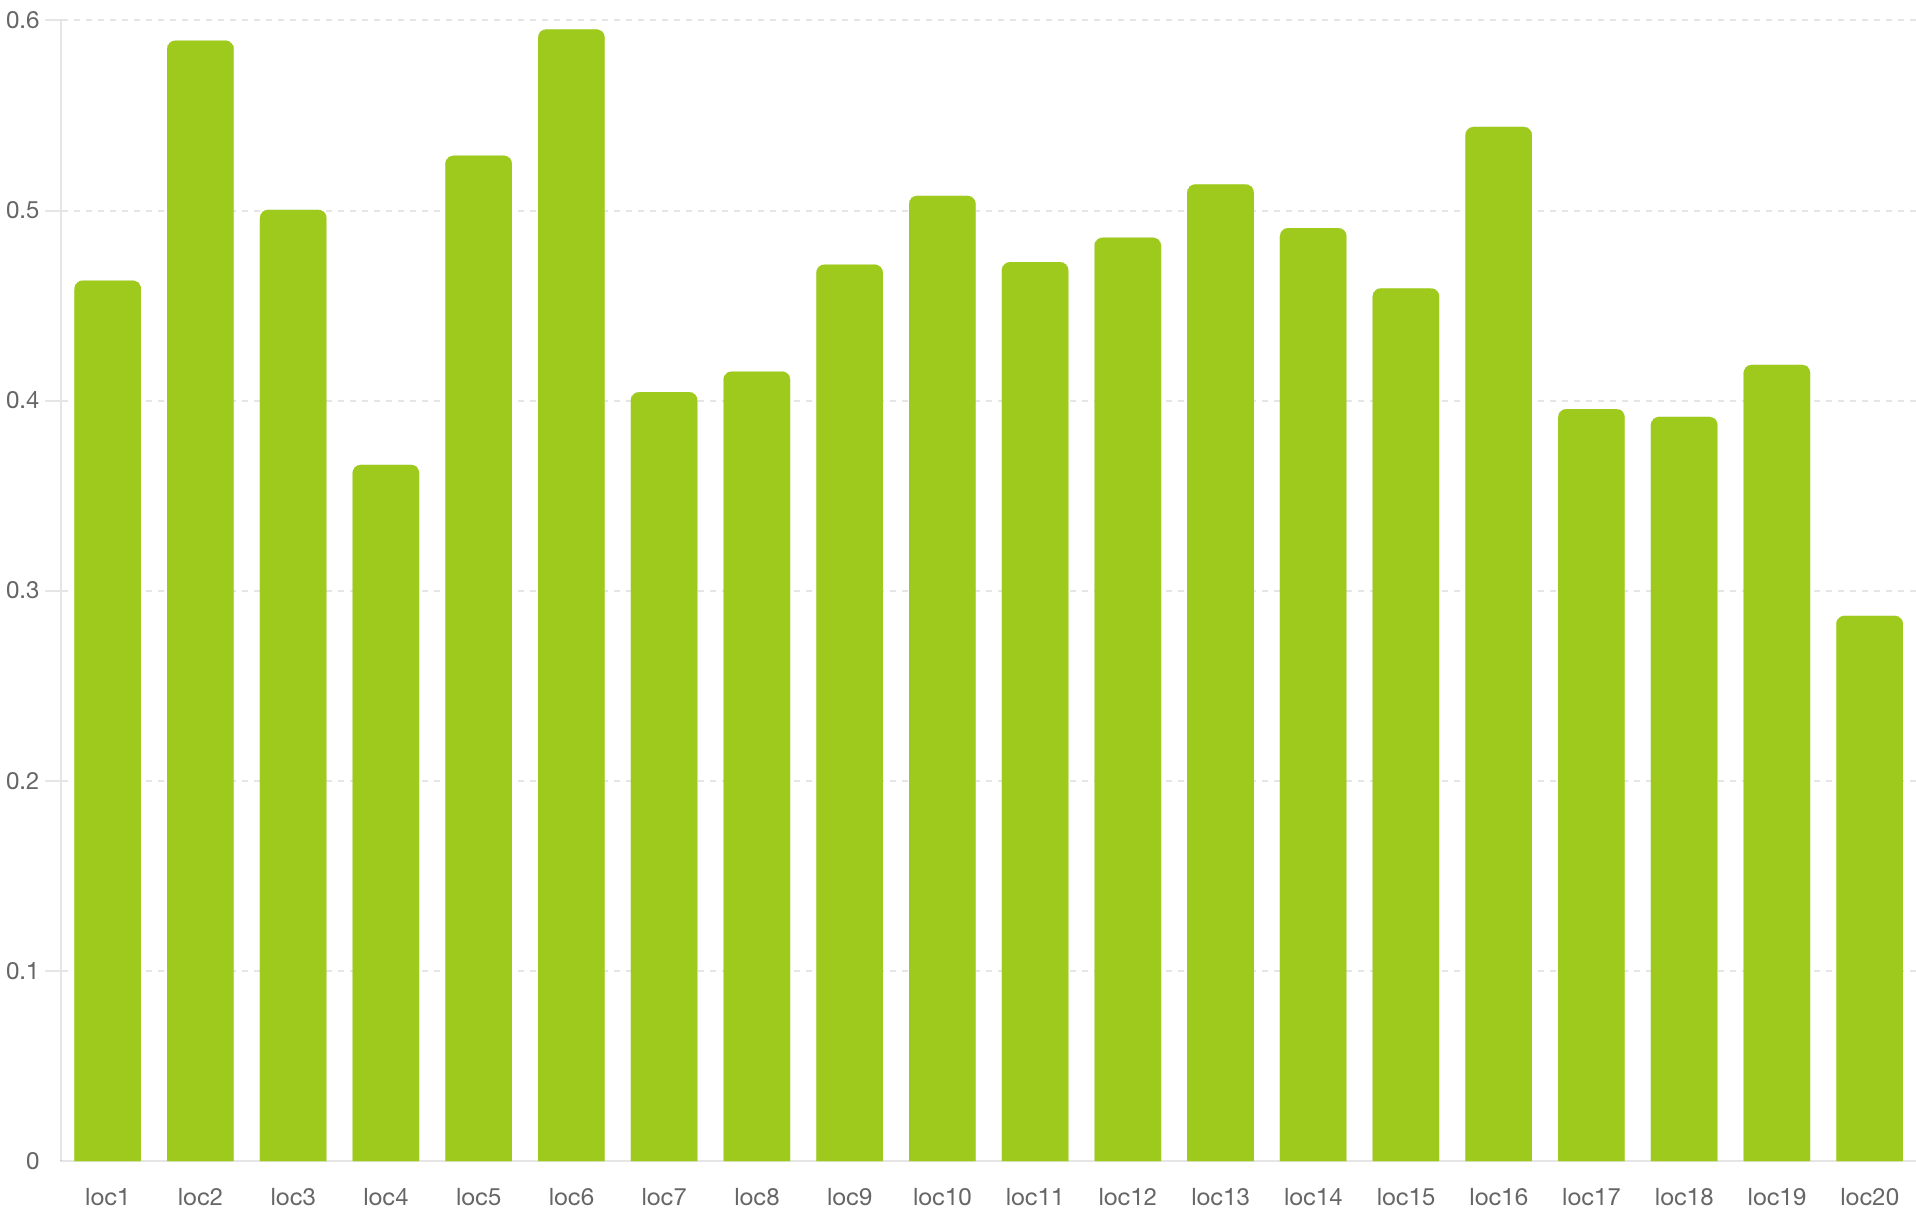
\includegraphics[width=\linewidth]{figs_compressed/nuplan-iou-locations.png}
    \caption{\textbf{IoU of \texttt{EmerSeg} compared to SegFormer across locations in Mapverse-nuPlan.}}
    \label{fig:iouvsloc-nuplan}
\end{figure}


\subsection{Qualitative Results}
We visualize some segmentation results in Fig.\ref{fig:vegas-loc1} to Fig.\ref{fig:vegas-loc6}. The visualizations highlight \texttt{EmerSeg}'s ability to accurately segment objects in complex traffic situations with multiple dynamic elements. These results underscore the versatility and reliability of our approach, showcasing its potential for real-world applications in autonomous driving and other vision-based tasks.

\begin{figure}[ht]
    \centering
    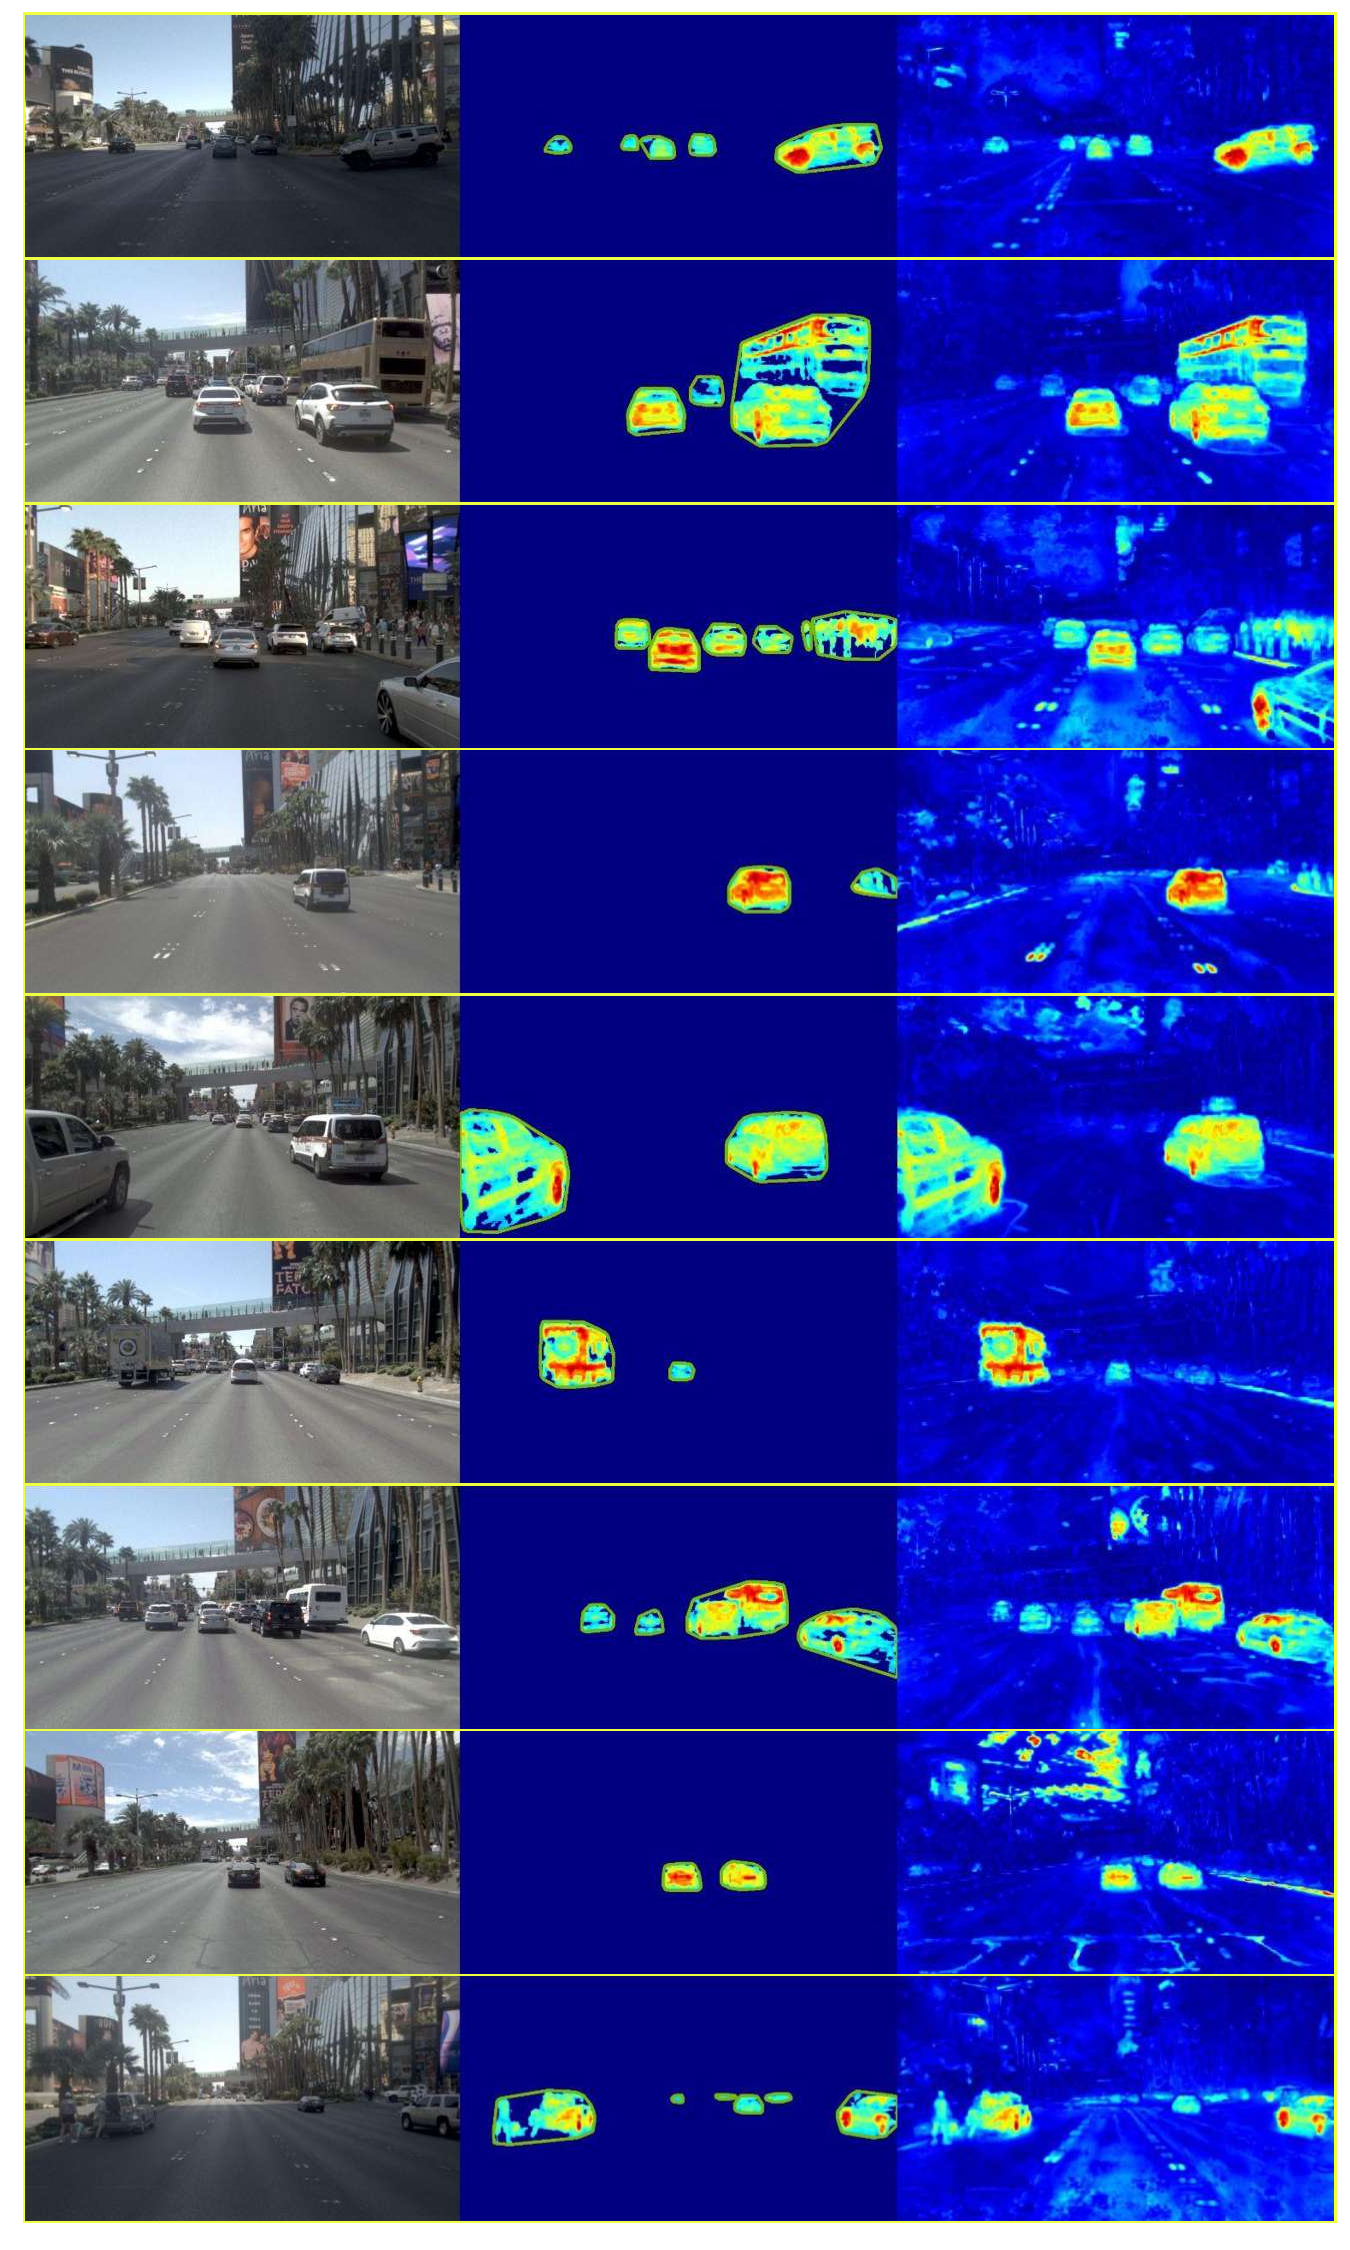
\includegraphics[width=0.88\linewidth]{figs_compressed/EmerSeg-loc1_compressed.pdf}
    \caption{\textbf{Qualitative results of \texttt{EmerSeg} for multiple traversals of location 1 of Mapverse-nuPlan.} From left to right: raw RGB image, extracted 2D ephemeral object masks, and normalized feature residuals visualized using a jet color map.}
    \label{fig:vegas-loc1}
\end{figure}

\begin{figure}[ht]
    \centering
    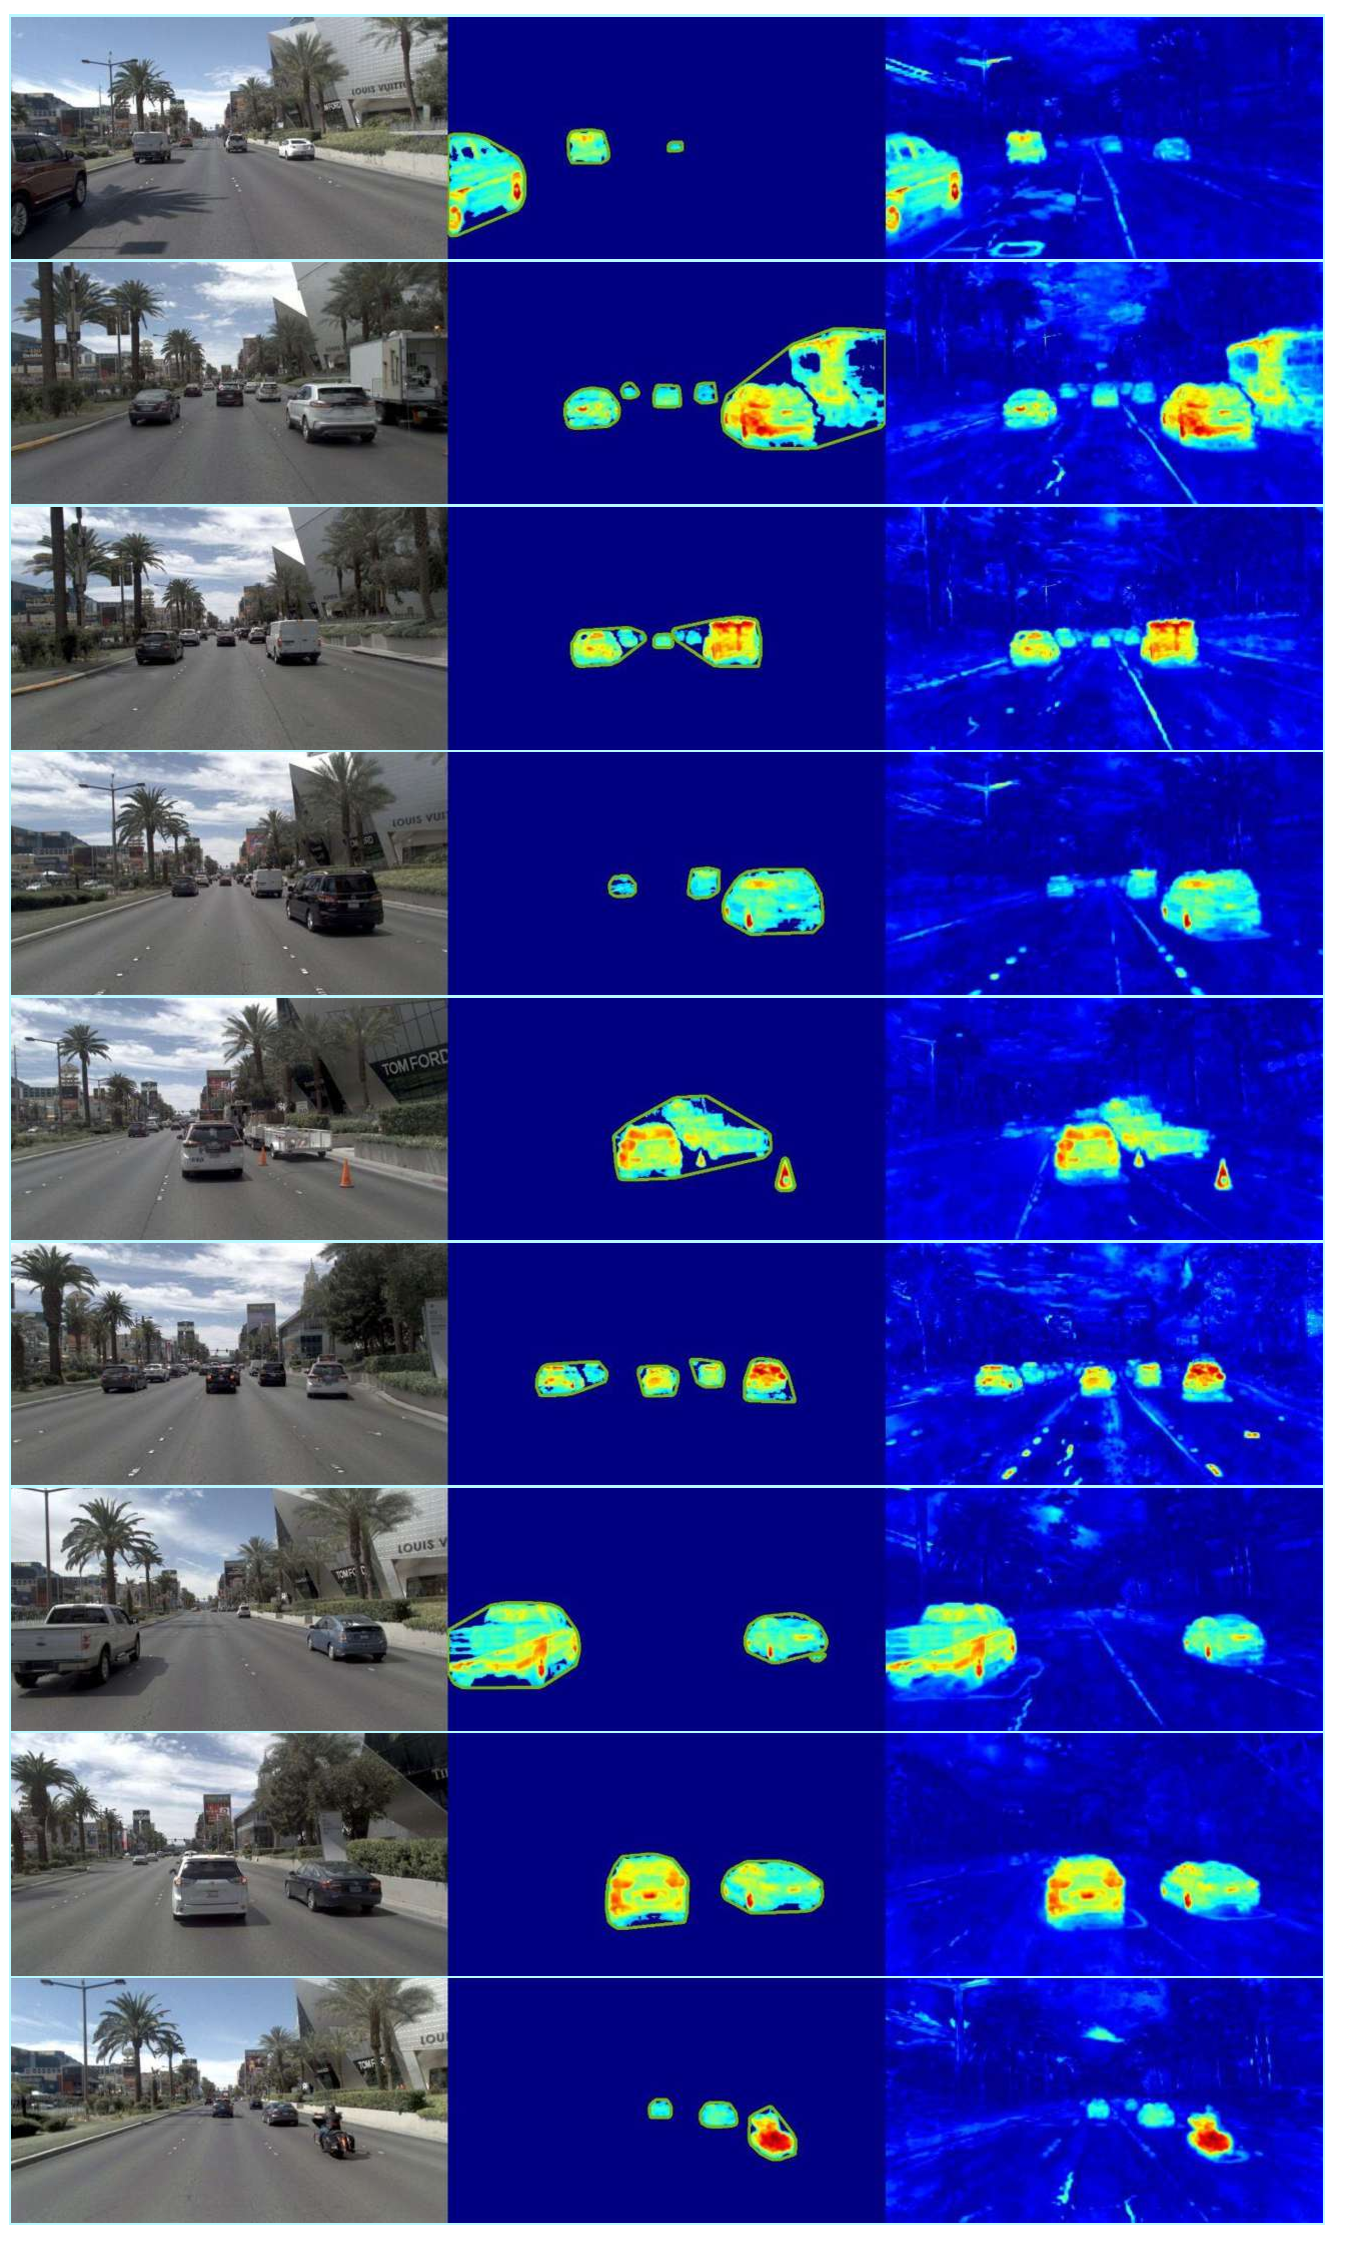
\includegraphics[width=0.88\linewidth]{figs_compressed/EmerSeg-loc2_compressed.pdf}
    \caption{\textbf{Qualitative results of \texttt{EmerSeg} for multiple traversals of location 2 of Mapverse-nuPlan.} From left to right: raw RGB image, extracted 2D ephemeral object masks, and normalized feature residuals visualized using a jet color map.}
    \label{fig:vegas-loc2}
\end{figure}

\begin{figure}[ht]
    \centering
    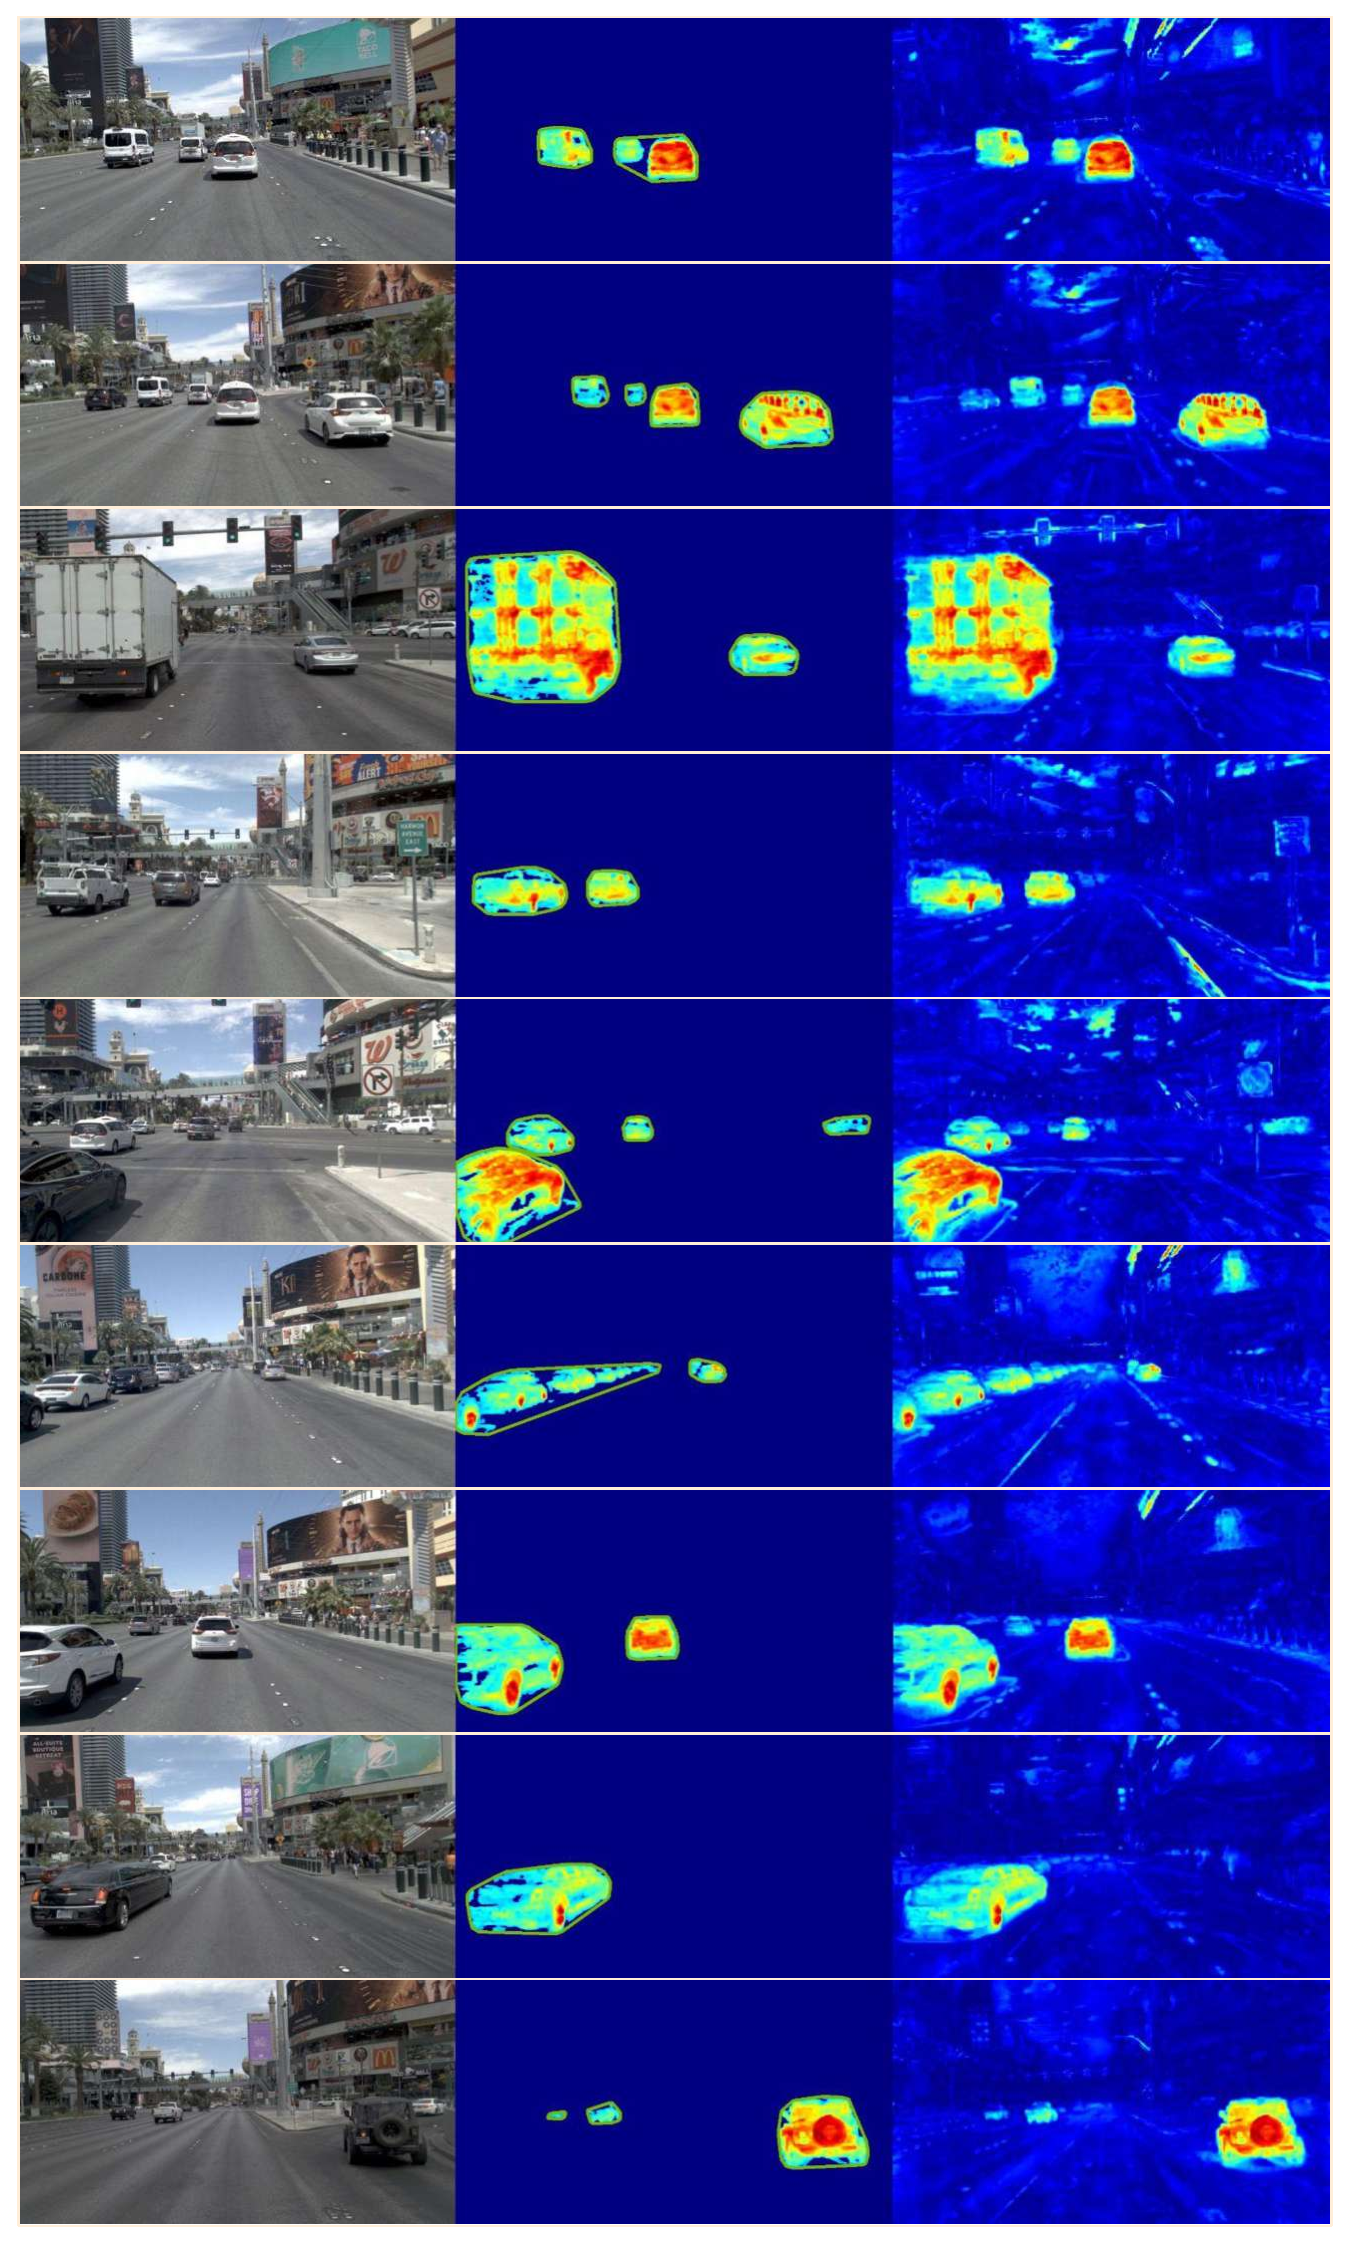
\includegraphics[width=0.88\linewidth]{figs_compressed/EmerSeg-loc3_compressed.pdf}
    \caption{\textbf{Qualitative results of \texttt{EmerSeg} for multiple traversals of location 3 of Mapverse-nuPlan.} From left to right: raw RGB image, extracted 2D ephemeral object masks, and normalized feature residuals visualized using a jet color map.}
    \label{fig:vegas-loc3}
\end{figure}

\begin{figure}[ht]
    \centering
    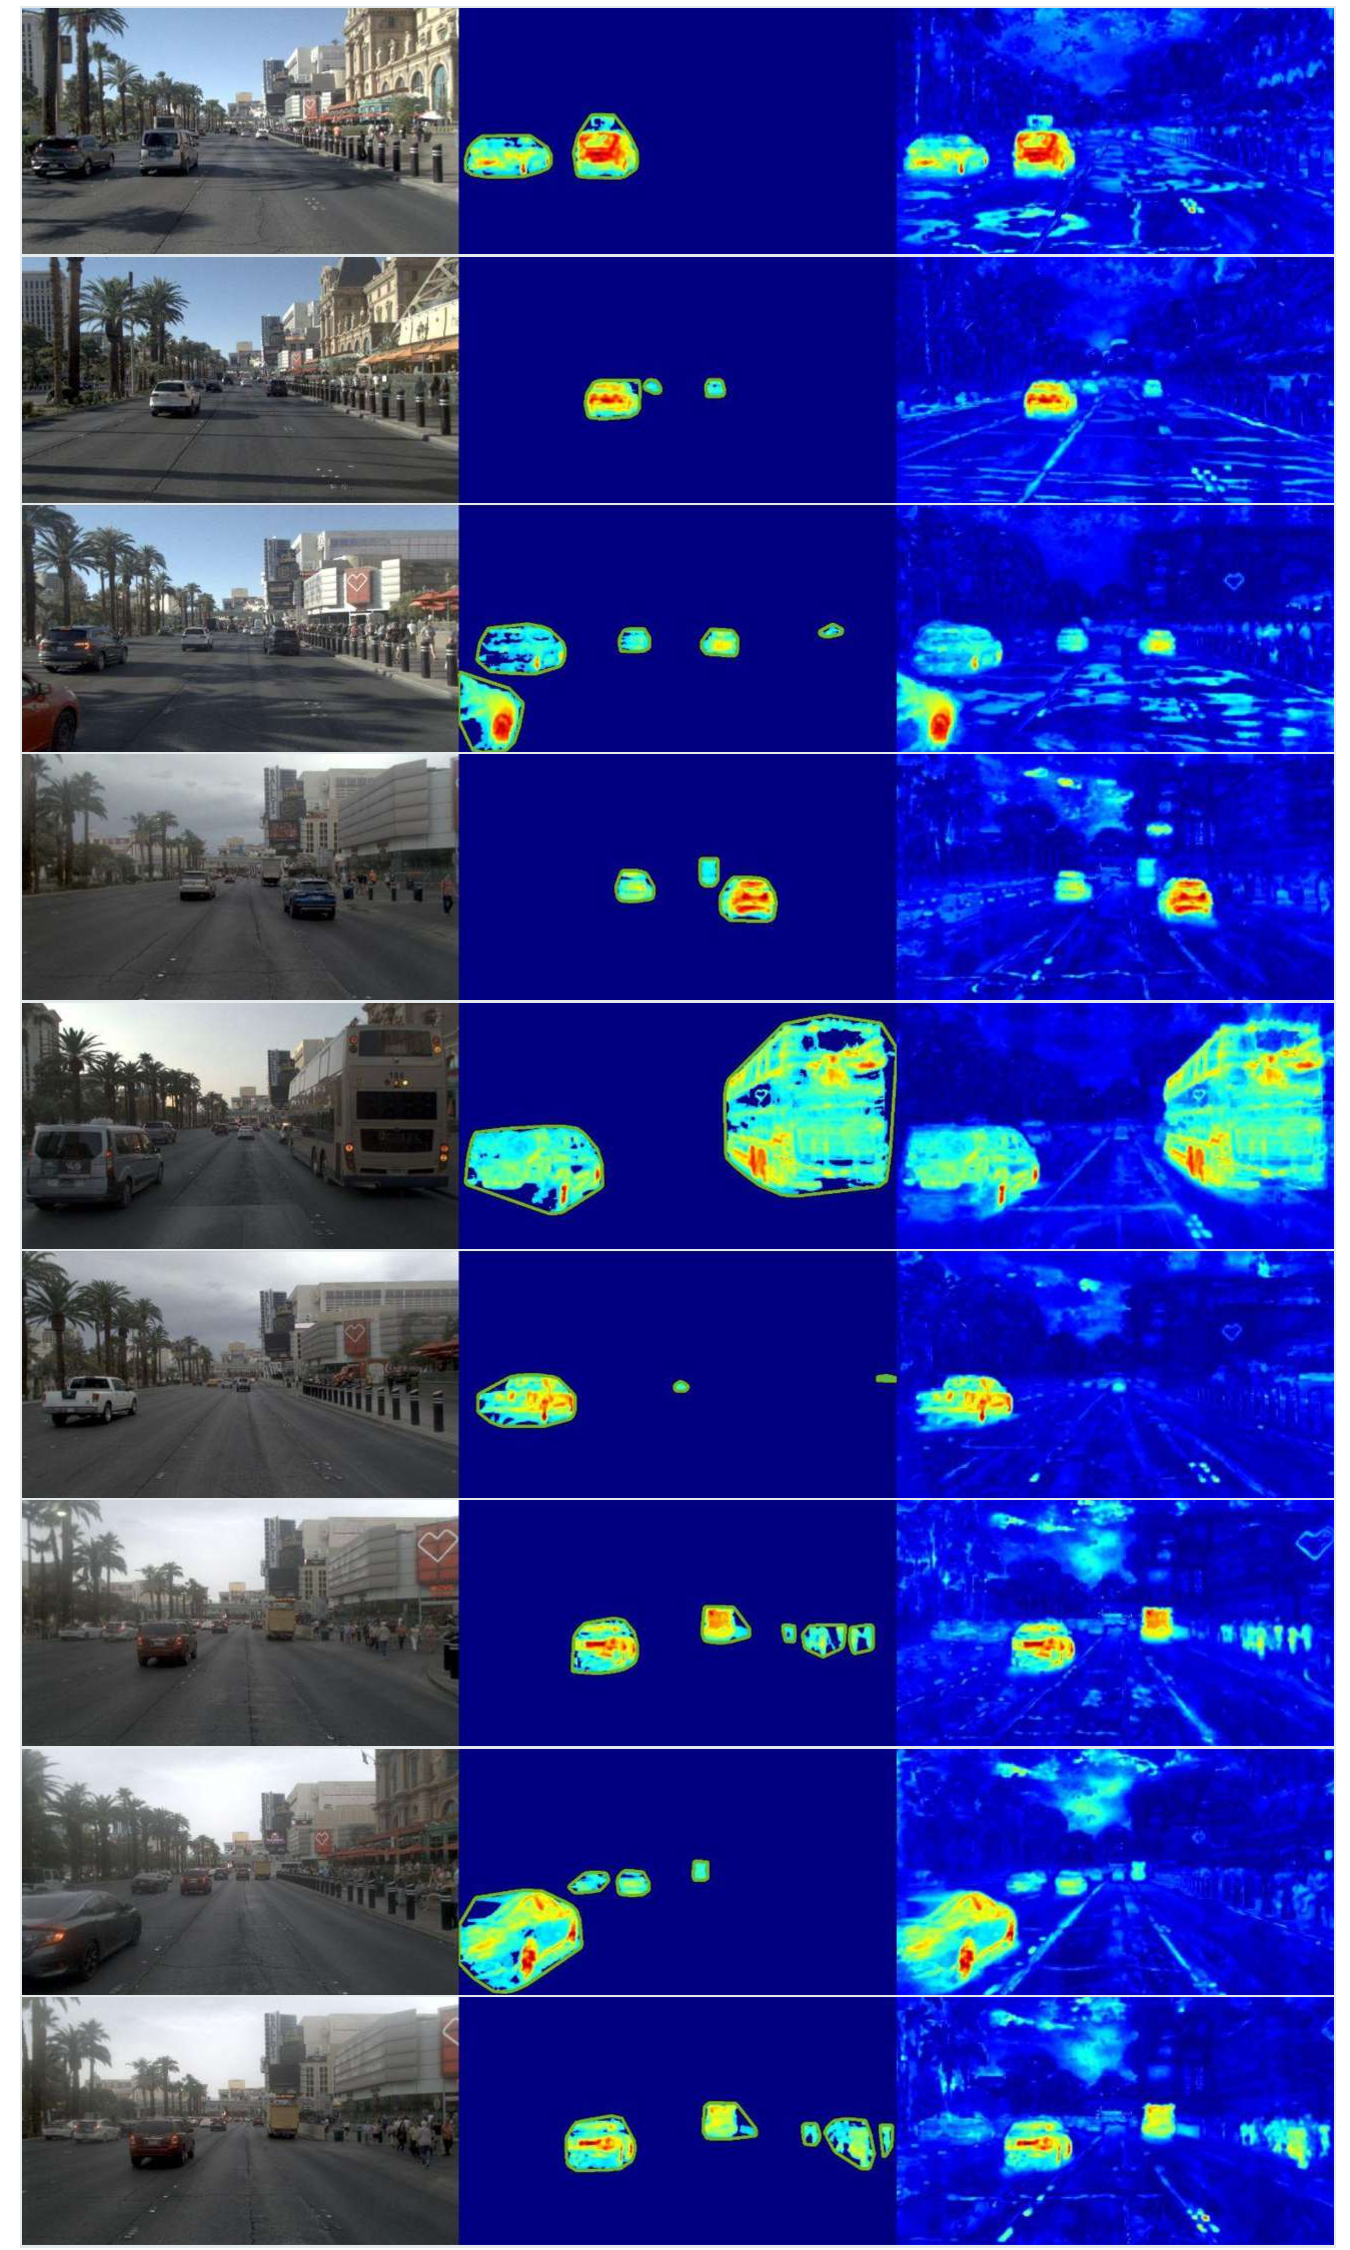
\includegraphics[width=0.88\linewidth]{figs_compressed/EmerSeg-loc4_compressed.pdf}
    \caption{\textbf{Qualitative results of \texttt{EmerSeg} for multiple traversals of location 4 of Mapverse-nuPlan.} From left to right: raw RGB image, extracted 2D ephemeral object masks, and normalized feature residuals visualized using a jet color map.}
    \label{fig:vegas-loc4}
\end{figure}

\begin{figure}[ht]
    \centering
    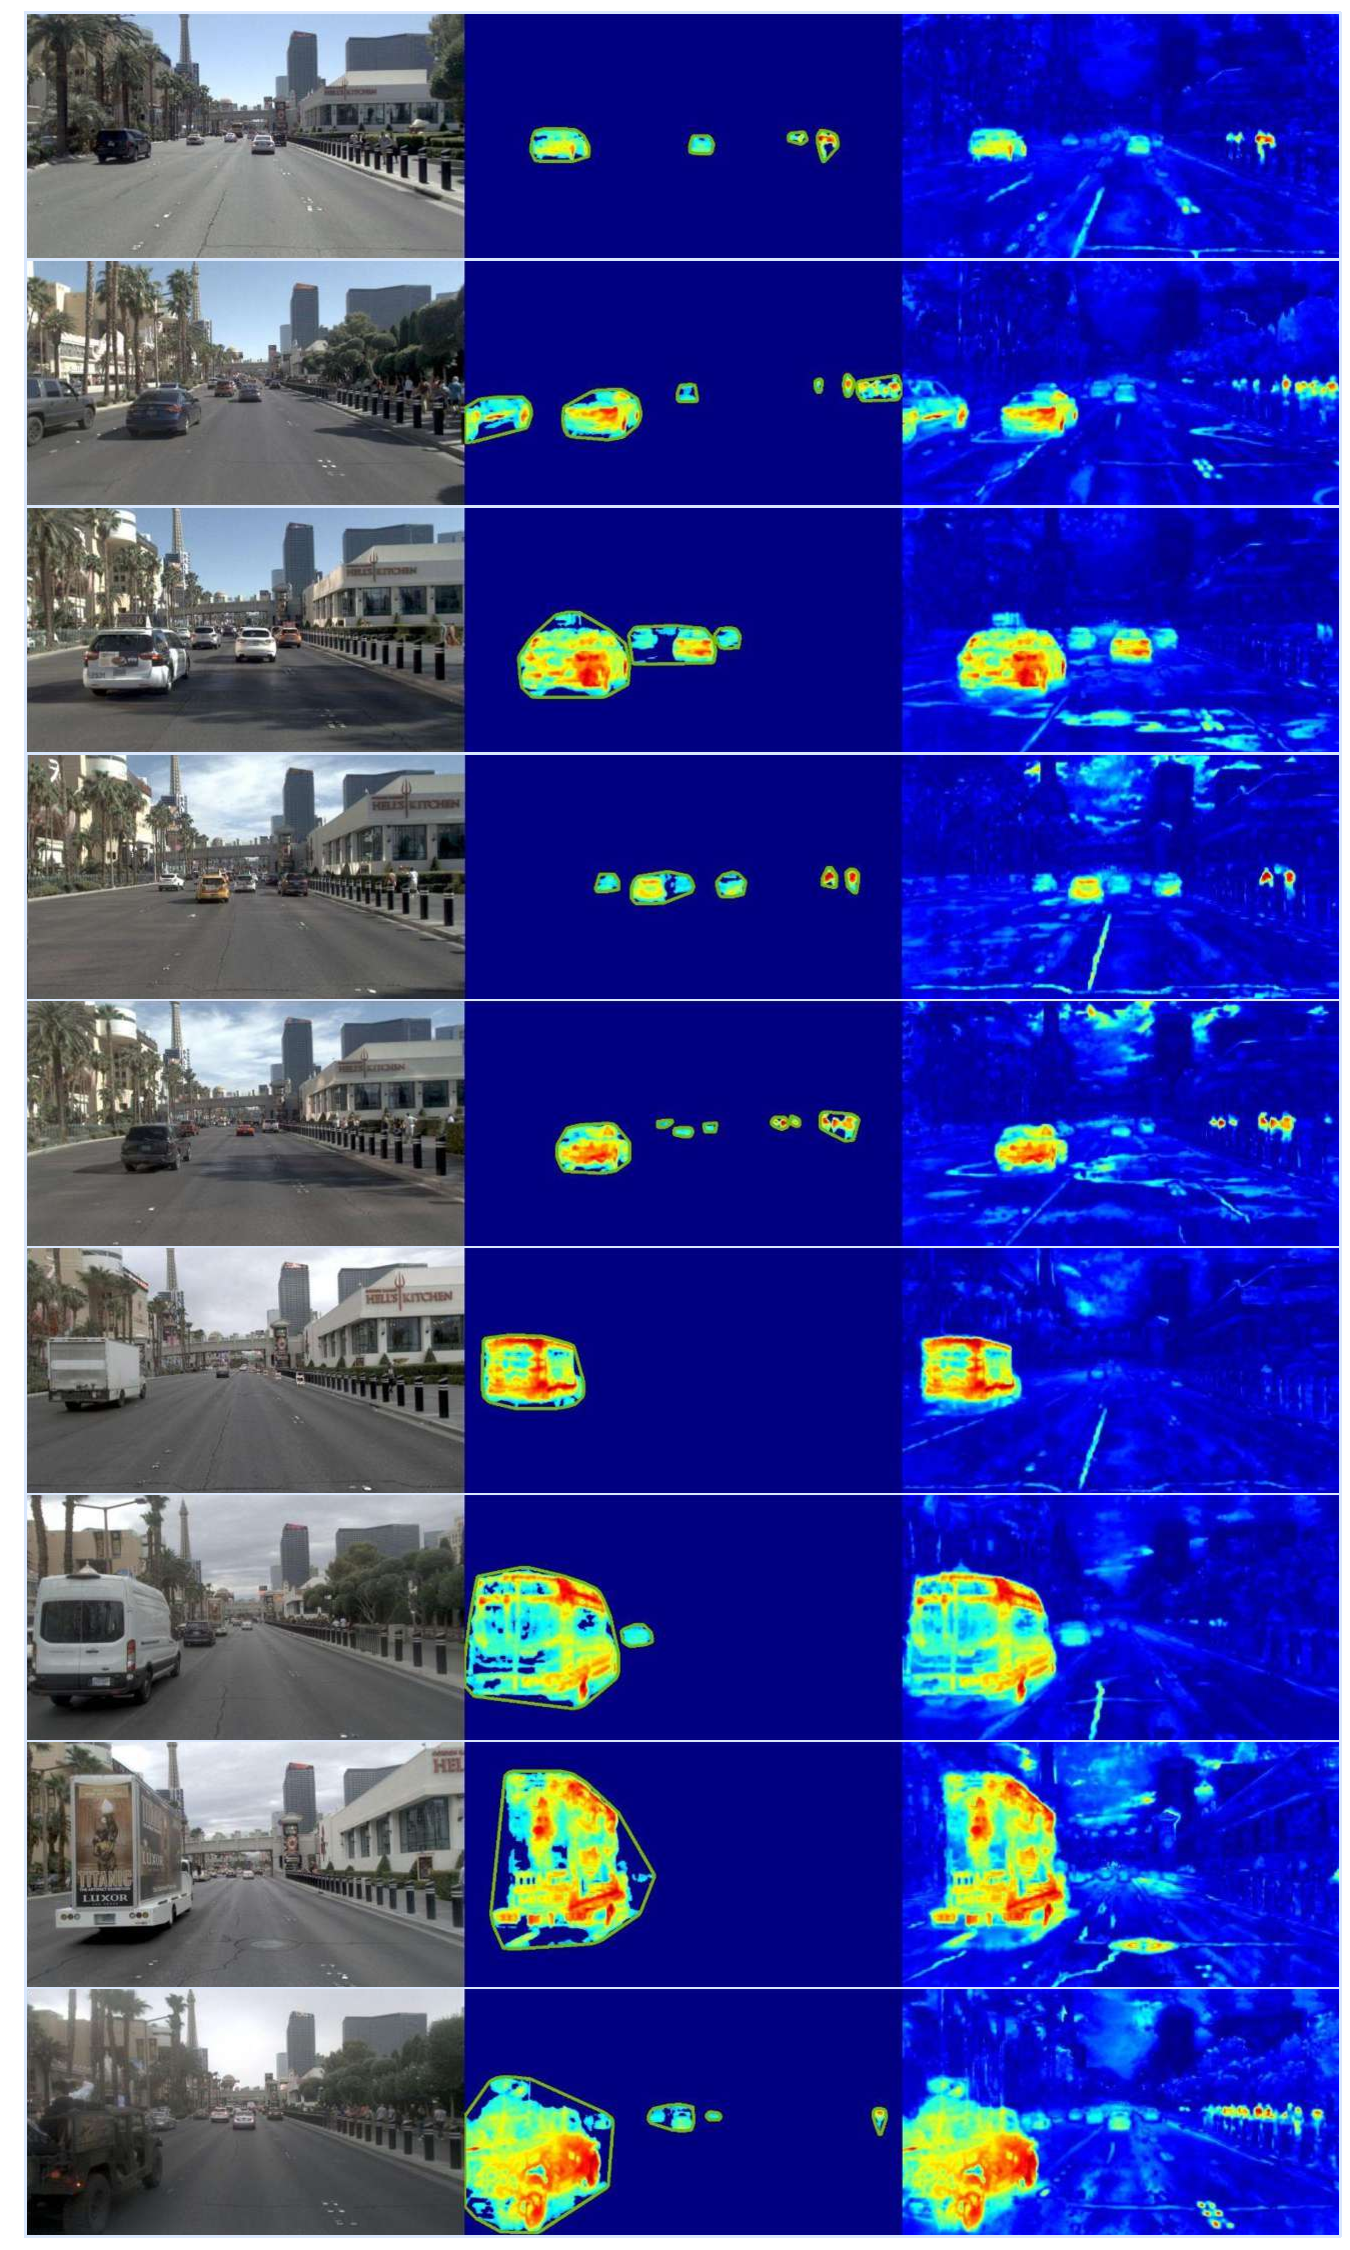
\includegraphics[width=0.88\linewidth]{figs_compressed/EmerSeg-loc5_compressed.pdf}
    \caption{\textbf{Qualitative results of \texttt{EmerSeg} for multiple traversals of location 5 of Mapverse-nuPlan.} From left to right: raw RGB image, extracted 2D ephemeral object masks, and normalized feature residuals visualized using a jet color map.}
    \label{fig:vegas-loc5}
\end{figure}

\begin{figure}[ht]
    \centering
    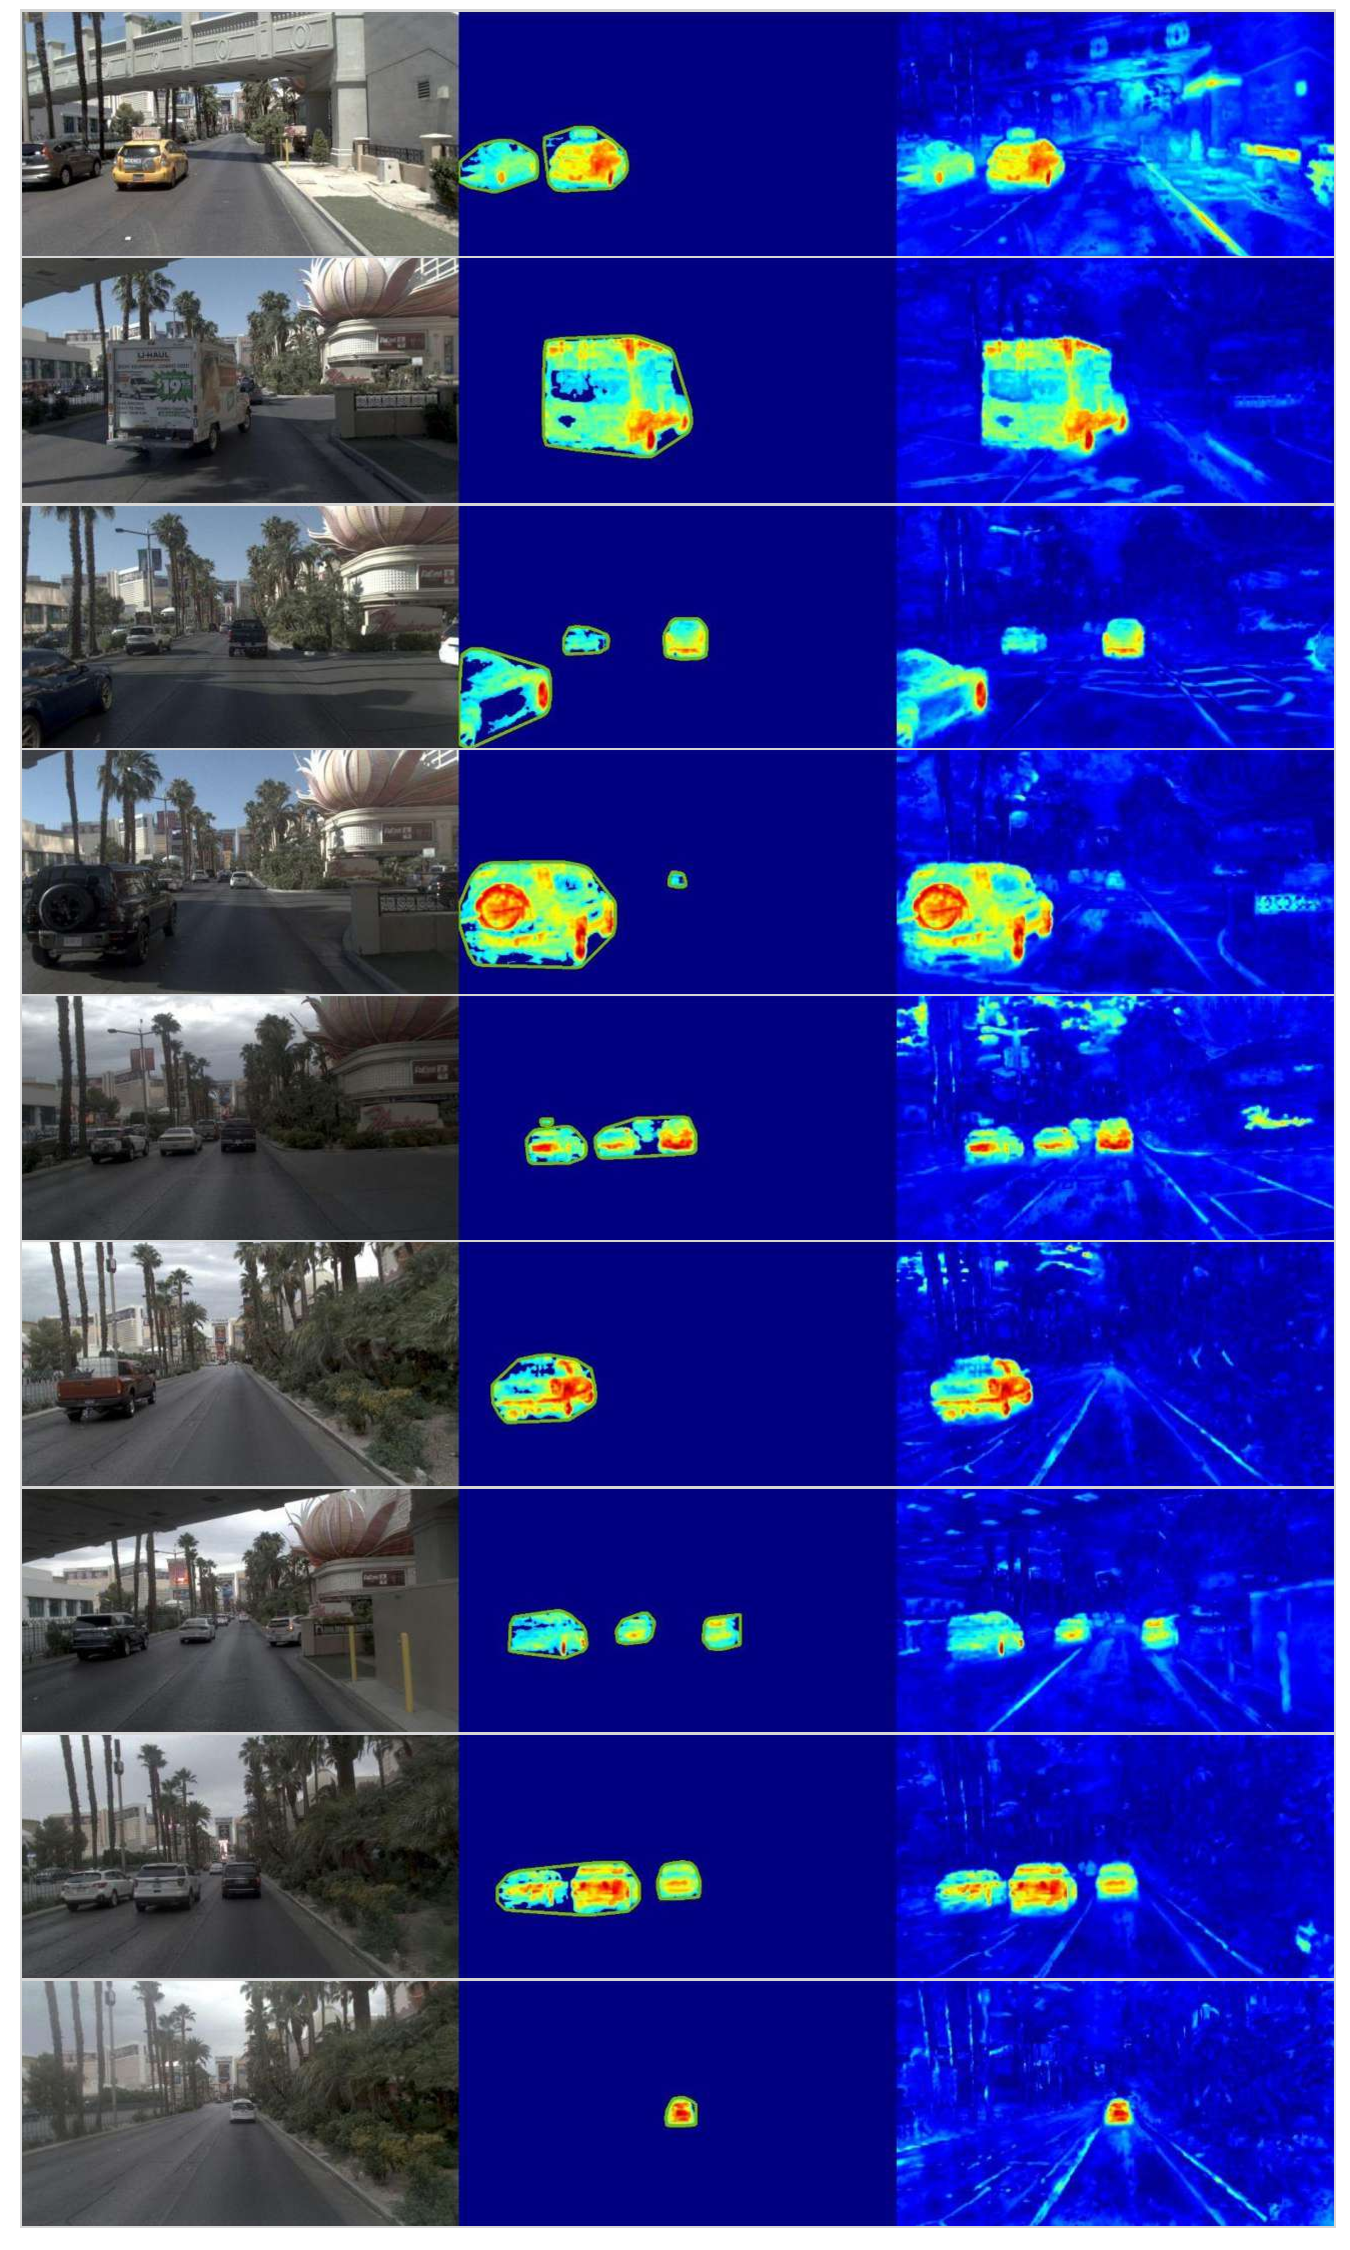
\includegraphics[width=0.88\linewidth]{figs_compressed/EmerSeg-loc6_compressed.pdf}
    \caption{\textbf{Qualitative results of \texttt{EmerSeg} for multiple traversals of location 6 of Mapverse-nuPlan.} From left to right: raw RGB image, extracted 2D ephemeral object masks, and normalized feature residuals visualized using a jet color map.}
    \label{fig:vegas-loc6}
\end{figure}



\clearpage
\section{Mapverse-nuPlan: Depth Visualization}
\label{sec:depth-nuplan-app}

\begin{figure}[ht]
\vspace{10mm}
    \centering
    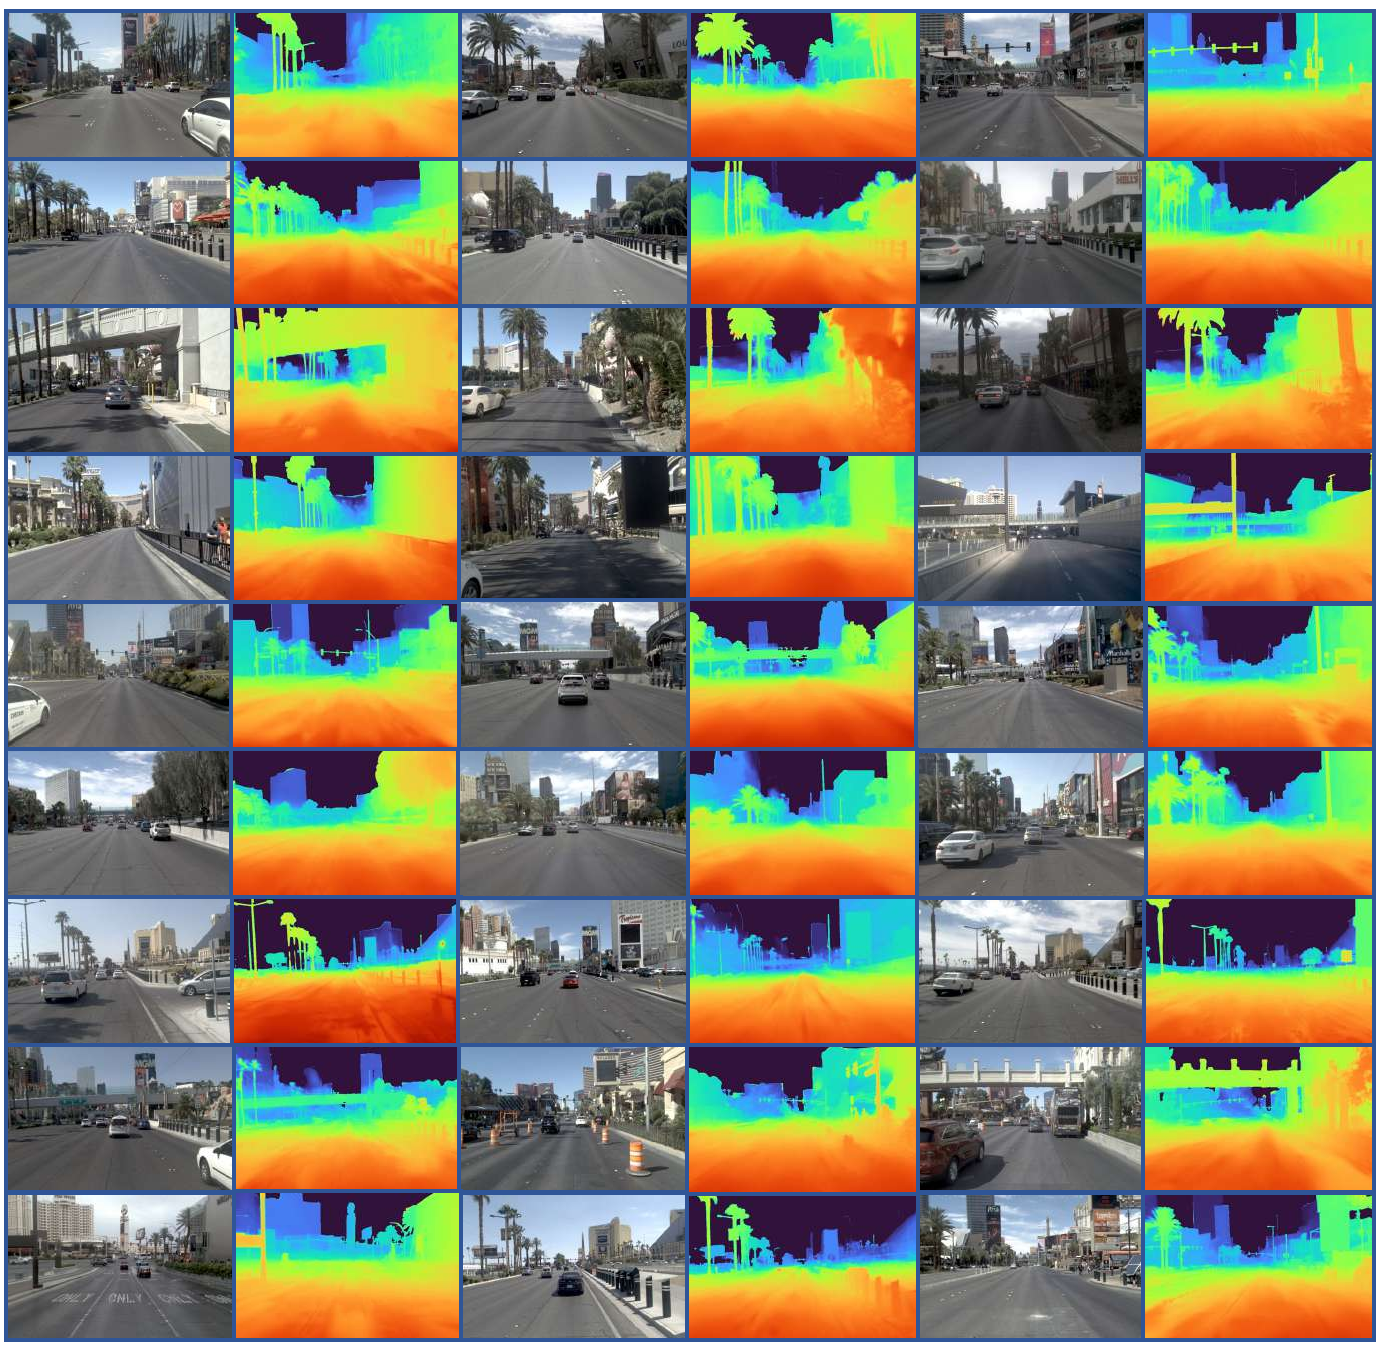
\includegraphics[width=\linewidth]{figs_compressed/nuplan-depth-app_compressed.pdf}
    \caption{\textbf{Visualizations of depth images in Mapverse-Ithaca365}}
    \label{fig:nuplan-depth-appendix}
\end{figure}


\clearpage
\section{Mapverse-nuPlan: Neural Rendering}
\label{sec:rendering-nuplan-app}

% Please add the following required packages to your document preamble:
% \usepackage{booktabs}
% \usepackage{multirow}
\begin{table}[ht]
\scriptsize
\centering
\caption{\textbf{Quantitative rendering results in Mapverse-nuPlan.} We set test/training views as 1/8. Pixels corresponding to transient objects are removed in the evaluations since we do not have ground truth background pixels in these regions occluded by transient objects.}
\begin{tabular}{@{}c|ccc|ccc|ccc@{}}
\toprule
\multirow{2}{*}{\textbf{Location}} & \multicolumn{3}{c|}{\textbf{3DGS}}                                 & \multicolumn{3}{c|}{\textbf{3DGS+SegFormer}}                      & \multicolumn{3}{c}{\textbf{EnvGS (Ours)}}                                 \\ \cmidrule(l){2-10} 
                                   & \multicolumn{1}{c|}{LPIPS ($\downarrow$)} & \multicolumn{1}{c|}{SSIM ($\uparrow$)} & PSNR ($\uparrow$)      & \multicolumn{1}{c|}{LPIPS ($\downarrow$)} & \multicolumn{1}{c|}{SSIM ($\uparrow$)} & PSNR ($\uparrow$)     & \multicolumn{1}{c|}{LPIPS ($\downarrow$)}& \multicolumn{1}{c|}{SSIM ($\uparrow$)} & PSNR ($\uparrow$)      \\ \midrule
1                                  & 0.177                     & 0.812                     & 21.94     & 0.164                      & 0.820                     & 21.99    & 0.167                     & 0.818                     & 21.88     \\
2                                  & 0.162                     & 0.836                     & 21.22     & 0.154                      & 0.840                     & 21.28    & 0.154                     & 0.839                     & 21.26     \\
3                                  & 0.173                     & 0.821                     & 20.59     & 0.165                      & 0.827                     & 20.77    & 0.164                     & 0.826                     & 20.77     \\
4                                  & 0.174                     & 0.843                     & 20.99     & 0.156                      & 0.850                     & 21.12    & 0.156                     & 0.849                     & 21.09     \\
5                                  & 0.160                     & 0.828                     & 19.82     & 0.143                      & 0.835                     & 20.20    & 0.144                     & 0.835                     & 20.17     \\
6                                  & 0.263                     & 0.765                     & 19.41     & 0.240                      & 0.778                     & 19.85    & 0.240                     & 0.778                     & 19.85     \\
7                                  & 0.232                     & 0.772                     & 18.92     & 0.228                      & 0.777                     & 18.55    & 0.227                     & 0.777                     & 18.56     \\
8                                  & 0.161                     & 0.823                     & 21.23     & 0.158                      & 0.825                     & 21.17    & 0.158                     & 0.825                     & 21.16     \\
9                                  & 0.171                     & 0.826                     & 20.77     & 0.161                      & 0.832                     & 20.98    & 0.162                     & 0.831                     & 20.97     \\
10                                 & 0.163                     & 0.844                     & 21.75     & 0.151                      & 0.854                     & 22.26    & 0.156                     & 0.850                     & 21.93     \\
11                                 & 0.179                     & 0.827                     & 20.86     & 0.169                      & 0.832                     & 21.08    & 0.170                     & 0.831                     & 21.06     \\
12                                 & 0.187                     & 0.815                     & 19.93     & 0.172                      & 0.824                     & 20.22    & 0.172                     & 0.824                     & 20.22     \\
13                                 & 0.253                     & 0.786                     & 19.74     & 0.239                      & 0.792                     & 19.98    & 0.241                     & 0.792                     & 19.96     \\
14                                 & 0.189                     & 0.798                     & 19.50     & 0.181                      & 0.803                     & 19.73    & 0.180                     & 0.804                     & 19.72     \\
15                                 & 0.224                     & 0.823                     & 20.58     & 0.193                      & 0.836                     & 20.99    & 0.194                     & 0.836                     & 20.99     \\
16                                 & 0.154                     & 0.846                     & 21.98     & 0.144                      & 0.851                     & 21.94    & 0.145                     & 0.851                     & 21.91     \\
17                                 & 0.171                     & 0.844                     & 21.73     & 0.153                      & 0.850                     & 21.67    & 0.158                     & 0.848                     & 21.59     \\
18                                 & 0.207                     & 0.803                     & 19.36     & 0.187                      & 0.811                     & 19.69    & 0.186                     & 0.812                     & 19.68     \\
19                                 & 0.212                     & 0.797                     & 19.18     & 0.206                      & 0.802                     & 18.99    & 0.206                     & 0.802                     & 19.02     \\
20                                 & 0.173                     & 0.840                     & 19.64     & 0.142                      & 0.854                     & 19.94    & 0.143                     & 0.854                     & 19.92     \\ \midrule
AVERAGE                            & 0.189                     & 0.818                     & 20.46     & 0.175                      & 0.825                     & 20.62    & 0.176                     & 0.824                     & 20.59     \\ \bottomrule
\end{tabular}
\end{table}

\begin{figure}[ht]
\vspace{1mm}
    \centering
    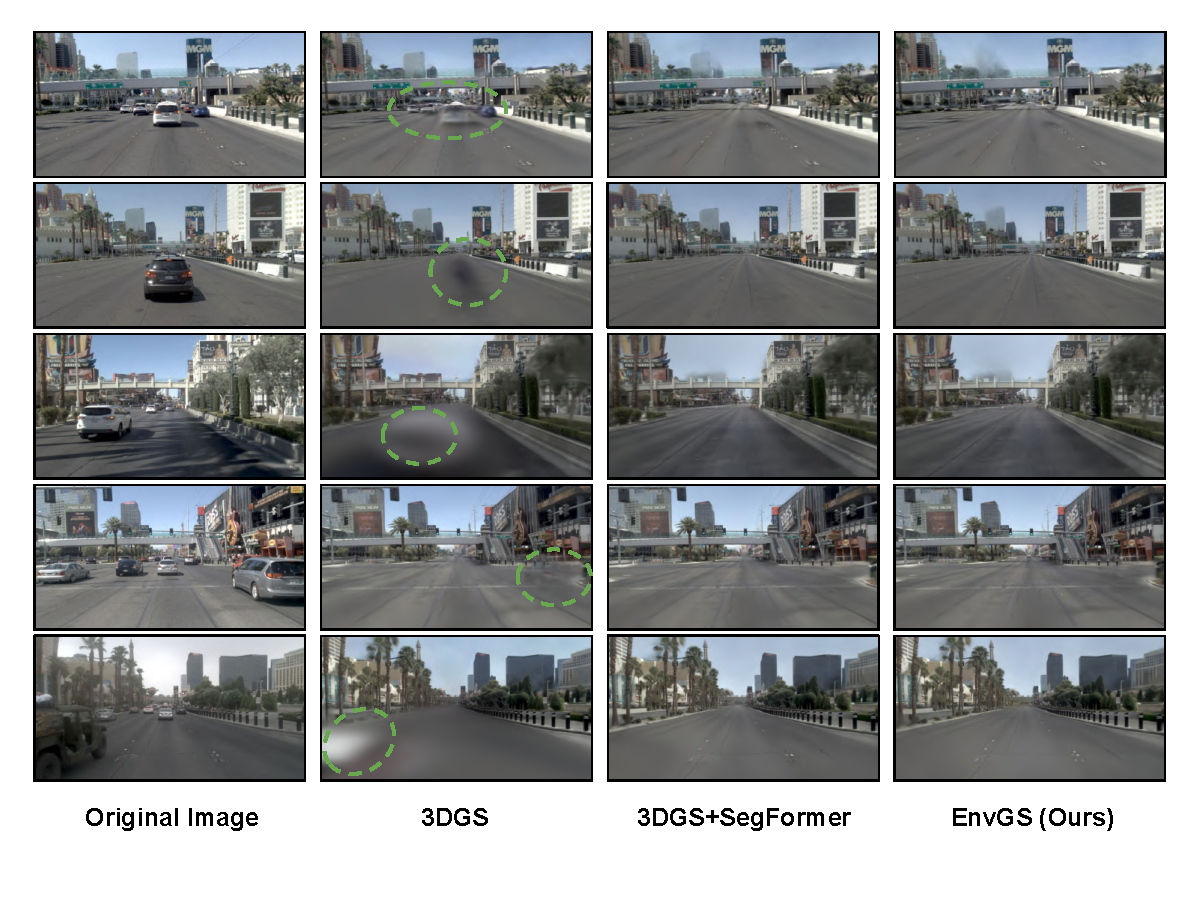
\includegraphics[width=0.925\linewidth]{figs_compressed/nuplan-rendering_compressed.pdf}
    \caption{\textbf{Visualizations of neural rendering in Mapverse-nuPlan.}}
    \label{fig:nuplan-rendering-appendix}
\end{figure}


\clearpage
\section{Limitations and Future Work}
\label{sec:limitation-appendix}

% \emph{(4)} \textit{Future improvements.} Future directions may include the exploration of more powerful foundation models and leveraging the temporal information within each traversal to enhance the consistency of the masks.

\subsection{Unsupervised 2D Segmentation}
\paragraph{Shadow segmentation} Figure~\ref{fig:limitation-shadow-appendix} illustrates the challenges encountered in accurately segmenting shadows. Each row represents different instances. The left column displays the original images, the middle column presents the segmentation output, and the right column highlights the areas where shadow removal failed, indicated by red circles. While there are some successful cases marked by green circles, our method lacks consistency across different scenes. 

\begin{figure}[ht]
    \centering
    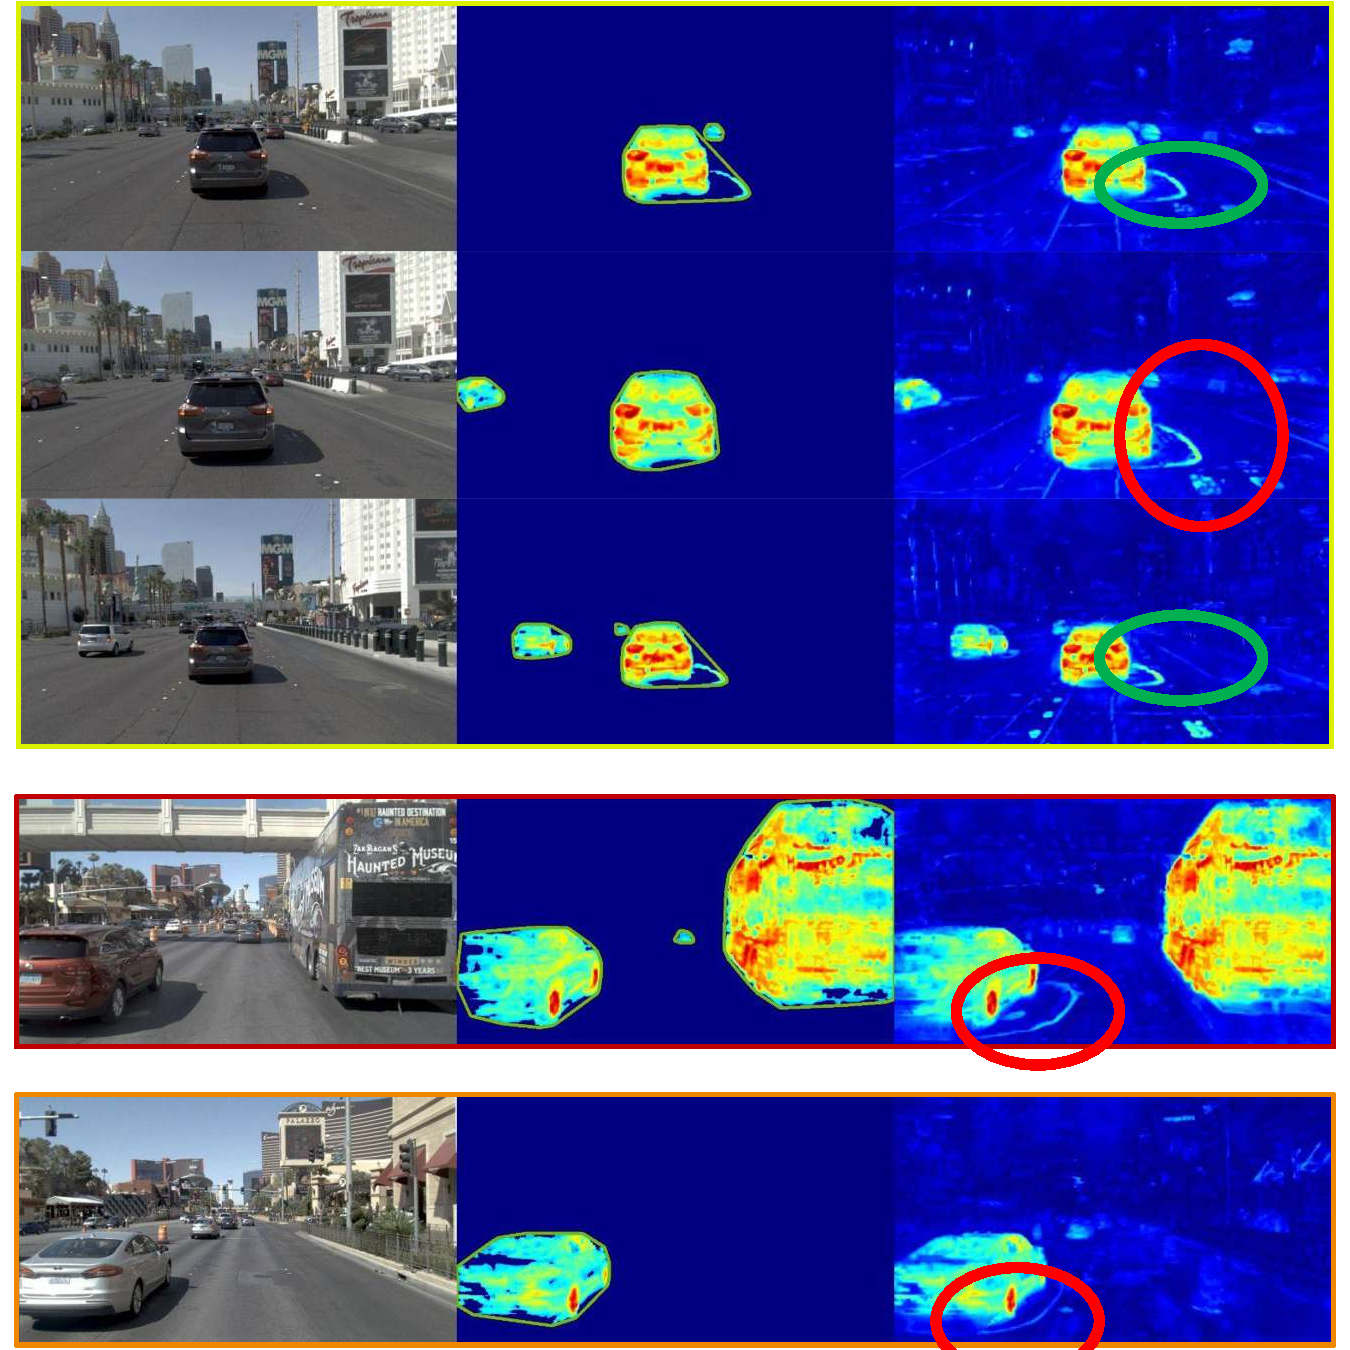
\includegraphics[width=0.66\linewidth]{figs_compressed/limitation-shadow_compressed.pdf}
    \caption{\textbf{Failure cases of shadow segmentation.}}
    \label{fig:limitation-shadow-appendix}
    \vspace{-2mm}
\end{figure}

 \paragraph{Large occluders} Figure~\ref{fig:limitation-large-appendix} illustrates the challenges faced when segmenting scenes with large and enduring occluders. When occluders occupy a significant portion of pixels and persist over time, our model tends to overfit to these occluders. This leads to a reduction in the feature residuals of the corresponding pixels, thereby failing the segmentation.

 \paragraph{Long-range objects} Figure~\ref{fig:limitation-small-appendix} highlights the challenges encountered when segmenting scenes with small and long-range objects. The red circles indicate regions where the segmentation algorithm struggles to differentiate these objects from their surroundings, often missing or inaccurately segmenting them. 

\paragraph{Reflective Surfaces} Figure~\ref{fig:limitation-reflect-appendix}  highlights the model's current limitations in handling reflective surfaces, which can vary significantly across traversals due to changes in lighting.
 
 \paragraph{Future Work} Future work will focus on developing better methods to robustly segment object shadows and leveraging temporal information to more effectively handle large and enduring occluders. Additionally, designing adaptive thresholds based on object distance will help better exploit the spatial information of the feature residuals. Furthermore, training a vision foundation model using large-scale, in-the-wild data will be crucial for enhancing the model's robustness.

\subsection{Geometry Reconstruction}

There are still challenges in road reconstruction, particularly due to the textureless nature of road surfaces. To address this, integrating advanced techniques such as mesh reconstruction~\cite{guedon2023sugar} and 2D Gaussian Splatting~\cite{Huang2DGS2024} could significantly enhance the geometric reconstruction capabilities of our method.  By enhancing the geometric fidelity of road surfaces, these techniques can help overcome the limitations posed by textureless areas, ensuring a more comprehensive and reliable mapping of driving environments.

\subsection{Neural Rendering}
Our method currently struggles with handling significant lighting variations and seasonal changes in the environment. Incorporating a 4D representation~\cite{yang2023gs4d,yan2024street}, which accounts for changes over time, could further enhance the quality of neural rendering. Additionally, we have not yet investigated very large-scale scene reconstruction. Incorporating recent Level-of-Detail (LOD) techniques can help address this large-scale problem~\cite{hierarchicalgaussians24}. We leave these as future works.

 \begin{figure}[ht]
    \centering
    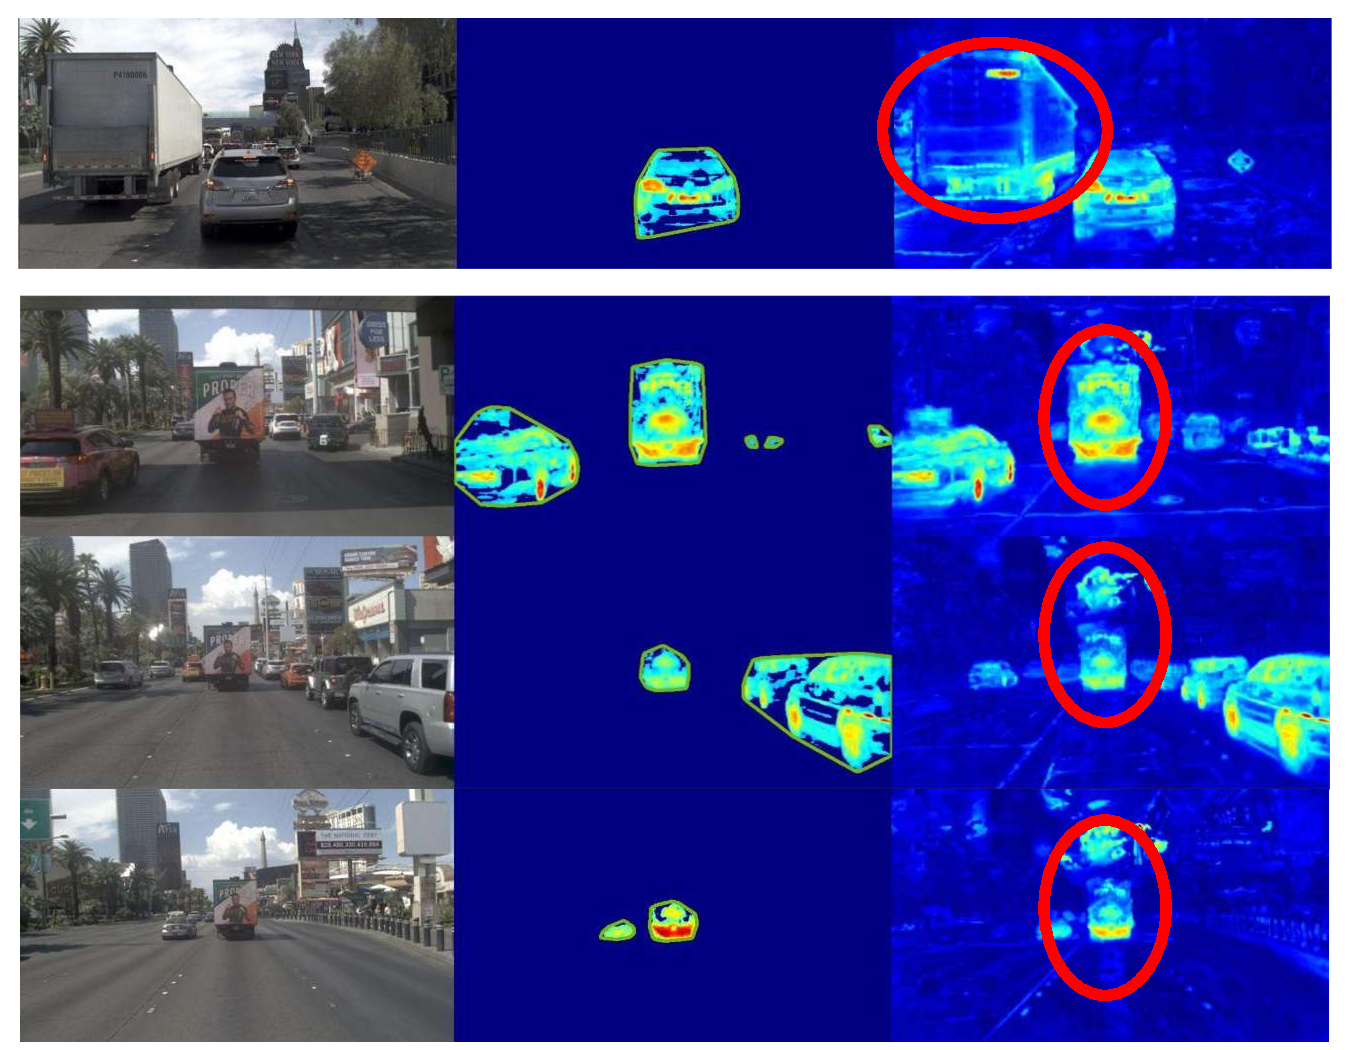
\includegraphics[width=0.66\linewidth]{figs_compressed/limitation-large_compressed.pdf}
    \caption{\textbf{Failure cases when faced with large and enduring occluders.}}
    \label{fig:limitation-large-appendix}
\end{figure}
\begin{figure}[ht]
    \centering
    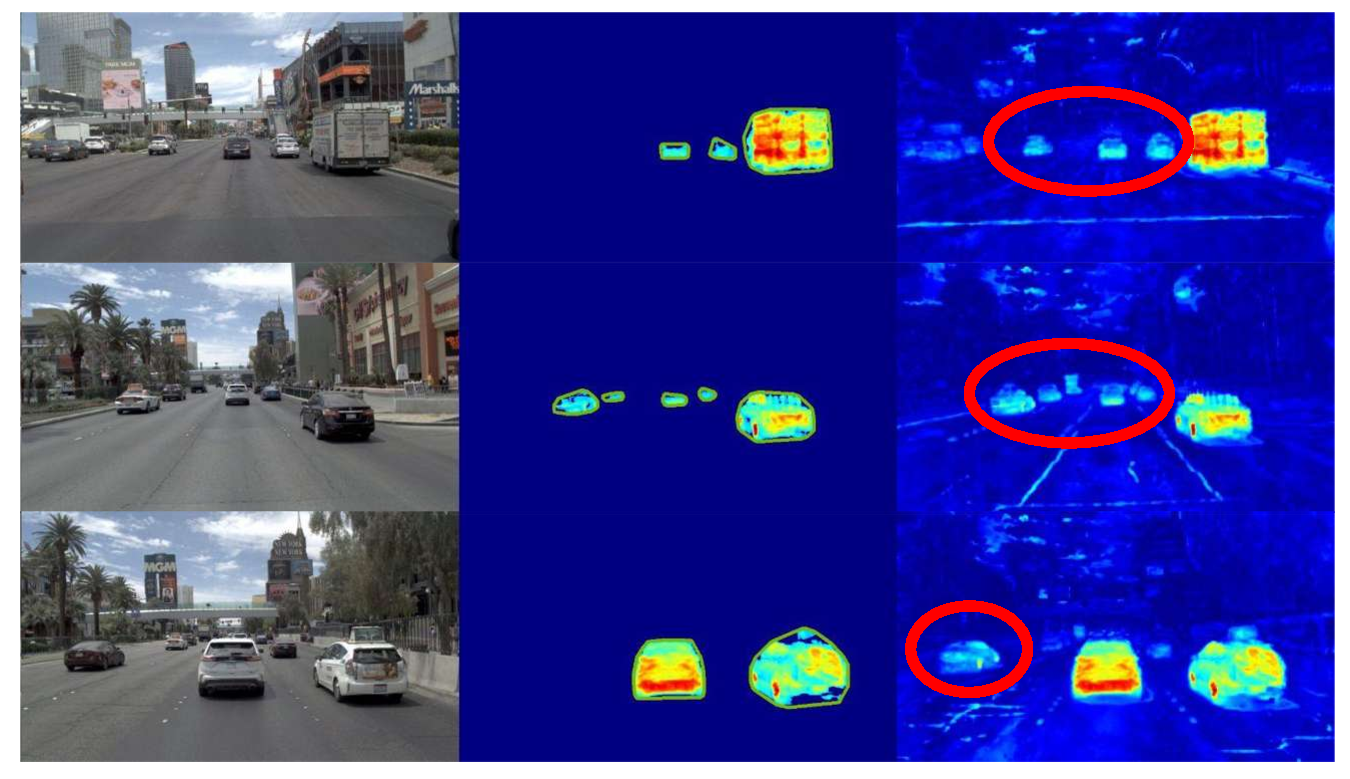
\includegraphics[width=0.66\linewidth]{figs_compressed/limitation-small_compressed.pdf}
    \caption{\textbf{Failure cases when faced with small and long-range objects.}}
    \label{fig:limitation-small-appendix}
\end{figure}
\begin{figure}[ht]
    \centering
    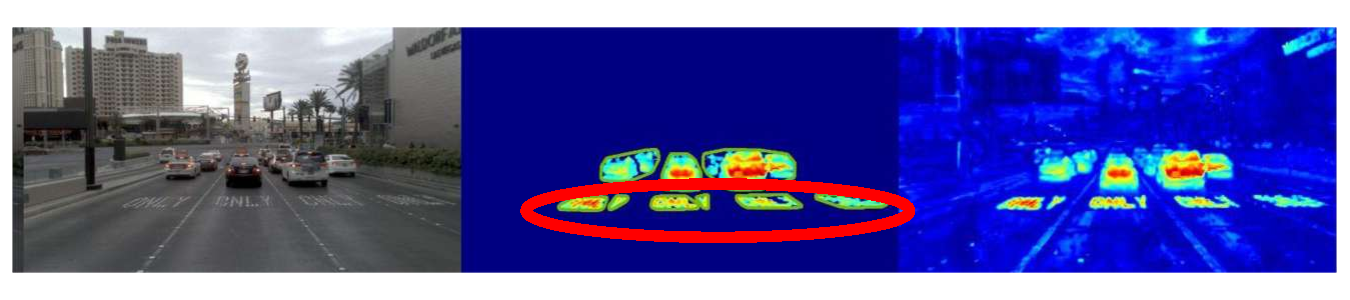
\includegraphics[width=0.66\linewidth]{figs_compressed/limitation-reflect_compressed.pdf}
    \caption{\textbf{Failure cases when faced with reflective surfaces.}}
    \label{fig:limitation-reflect-appendix}
\end{figure}


\end{document}
